%\documentclass[10pt,preprint]{aastex}
\documentclass[iop]{emulateapj}
%\usepackage{epsfig}
%\usepackage{changebar}
%\usepackage{natbib}
%\usepackage{lscape}

%\topmargin -0.0in
\def\boldsymbol{\bf}
\newcommand{\tnm}{\tablenotemark}
\newcommand{\tnt}{\tablenotetext}

\bibpunct{(}{)}{;}{a}{}{,}

\slugcomment{To be submitted to the ApJ}

\shorttitle{ALMA Imaging of {\it Herschel} DSFGs}
\shortauthors{Bussmann et al.}

%\usepackage{amsmath}
%\usepackage{amssymb}

%\long\def\symbolfootnote[#1]#2{\begingroup%
%\def\thefootnote{\fnsymbol{footnote}}\footnote[#1]{#2}\endgroup} 
%\long\def\symbolfootnote[#1]#2{\begingroup\def\thefootnote{\fnsymbol{footnote}}
%\footnote[#1]{#2}\endgroup}


\begin{document}

\title{HerMES: Spatially resolved ALMA Imaging of {\it
Herschel}$^{\dagger}$-selected Dusty Star-forming Galaxies}

%shortlensing:[hda fdb hf aih mk alapi ao dr jw]

%./authors_list hermes_authors_data_dr1_20121108.txt apj rsb dr fialkov hayward cowley almalens

\author{R.~S.~Bussmann\altaffilmark{1},
D.~Riechers\altaffilmark{1},
A.~Fialkov\altaffilmark{2},
C.~Hayward\altaffilmark{3,4},
W.~Cowley\altaffilmark{5},
J.~Bock\altaffilmark{6,7},
J.~Calanog\altaffilmark{8},
A.~Cooray\altaffilmark{8},
F.~De Bernardis\altaffilmark{8},
R.~Hopwood\altaffilmark{9},
M.~Jarvis\altaffilmark{10},
C.~Lacey\altaffilmark{5},
A.~Loeb\altaffilmark{4},
S.~J.~Oliver\altaffilmark{11},
I.~P{\'e}rez-Fournon\altaffilmark{12,13},
I.~G.~Roseboom\altaffilmark{11,14},
A.~J.~Smith\altaffilmark{11},
L.~Wang\altaffilmark{11},
J.~Wardlow\altaffilmark{15}}
\altaffiltext{1}{Department of Astronomy, Space Science Building, Cornell University, Ithaca, NY, 14853-6801}
\altaffiltext{2}{Departement de Physique, Ecole Normale Sup erieure, CNRS, 24 rue Lhomond, Paris, 75005 France}
\altaffiltext{3}{TAPIR 350-17, California Institute of Technology, 1200 E. California Boulevard, Pasadena, CA 91125}
\altaffiltext{4}{Harvard-Smithsonian Center for Astrophysics, 60 Garden Street, Cambridge, MA 02138}
\altaffiltext{5}{Institute for Computational Cosmology, Department of Physics, University of Durham, South Road, Durham, DH1 3LE, UK}
\altaffiltext{6}{California Institute of Technology, 1200 E. California Blvd., Pasadena, CA 91125}
\altaffiltext{7}{Jet Propulsion Laboratory, 4800 Oak Grove Drive, Pasadena, CA 91109}
\altaffiltext{8}{Dept. of Physics \& Astronomy, University of California, Irvine, CA 92697}
\altaffiltext{9}{Astrophysics Group, Imperial College London, Blackett Laboratory, Prince Consort Road, London SW7 2AZ, UK}
\altaffiltext{10}{Centre for Astrophysics Research, University of Hertfordshire, College Lane, Hatfield, Hertfordshire AL10 9AB, UK}
\altaffiltext{11}{Astronomy Centre, Dept. of Physics \& Astronomy, University of Sussex, Brighton BN1 9QH, UK}
\altaffiltext{12}{Instituto de Astrof{\'\i}sica de Canarias (IAC), E-38200 La Laguna, Tenerife, Spain}
\altaffiltext{13}{Departamento de Astrof{\'\i}sica, Universidad de La Laguna (ULL), E-38205 La Laguna, Tenerife, Spain}
\altaffiltext{14}{Institute for Astronomy, University of Edinburgh, Royal Observatory, Blackford Hill, Edinburgh EH9 3HJ, UK}
\altaffiltext{15}{Dark Cosmology Centre, Niels Bohr Institute, University of Copenhagen, Juliane Maries Vej 30, 2100 Copenhagen, Denmark}



%\newpage

\begin{abstract}

    The {\it Herschel} Multi-tiered Extragalactic Survey (HerMES) has
    identified large numbers of dusty star-forming galaxies (DSFGs) over a wide
    range in redshift.  A detailed understanding of these DSFGs is hampered by
    the poor spatial resolution of {\it Herschel}.  We present 870$\,\mu$m
    0$\farcs$45 imaging obtained in Cycle~0 with the Atacama Large
    Millimeter/submillimeter Array (ALMA) of a sample of 29 HerMES DSFGs.  We
    identify a total of 62 sources down to the $5\sigma$ limit in our ALMA
    sample ($\sigma \approx 0.2\,$mJy).  Optical or near-infrared imaging
    indicates that 36 of the ALMA sources experience a significant flux boost
    from gravitational lensing ($\mu > 1.1$), but only 6 are strongly lensed
    and show multiple images.  We introduce and make use of {\sc uvmcmcfit}, a
    general purpose and publicly available Markov Chain Monte Carlo visibility
    plane analysis tool to analyze the source properties.  Nearly 70\% of the
    {\it Herschel} sources break down into multiple ALMA counterparts,
    consistent with previous research indicating that the multiplicity rate is
    high in bright sources discovered in sub-mm or FIR surveys with poor
    spatial resolution.  The ALMA counterparts to our {\it Herschel} targets
    are located much closer to each other than ALMA counterparts to sources
    found in the LABOCA ECDFS Submillimeter Survey.  Theoretical models
    underpredict the excess in number of sources with small separations from
    each other that is seen in our ALMA sample.  Combined with our previous
    work on brighter {\it Herschel} sources, the lens models presented here
    constrain the shape of the intrinsic luminosity function for DSFGs to have
    a break around 8$\,$mJy with a very steep fall off at higher flux
    densities.  The high multiplicity rate and low projected separations
    between sources seen in our sample argue in favor of interactions and
    mergers driving the prodigious emission from the brightest DSFGs.

\end{abstract}

\keywords{galaxies: evolution --- galaxies: fundamental parameters --- 
galaxies: high-redshift}


%\newpage

\section{Introduction} \label{sec:intro} 

Galaxies selected in blind surveys at far-infrared (FIR) or sub-millimieter
(sub-mm) wavelengths are generally known as dusty star-forming galaxies
(DSFGs).  They cover a wide range in redshift from $z \sim 0.5$ to $z > 6$
\citep{2005ApJ...622..772C, Casey:2012qy, Messias:2014fk, Riechers:2013lr},
with a significant component at $z \sim 2$ \citep{Casey:2012uq,
Bothwell:2013lr}, when they represent the most FIR-luminous objects in
existence during this epoch.   They are signposts of significant over-densities
\citep{Daddi:2009qy, Capak:2011qy} and likely represent
the formative stages of the most massive elliptical galaxies found in the local
Universe \citep[e.g.,][]{Ivison:2013fk, Fu:2013lr}.  Moreover, they constitute
an important component of the overall galaxy population at $z \sim 2$
\citep[e.g.,][]{Magnelli:2011ul}, when the star-formation rate density in
the Universe peaked \citep[e.g.,][]{Lilly:1996uq, 1996MNRAS.283.1388M}.  

Our collective understanding of DSFGs is currently taking a dramatic leap
forward thanks in large part to the advent of the {\it Herschel Space
Observatory} \citep[{\it Herschel};][]{Pilbratt:2010fk}.  This has resulted in
a revolution in the size and depth of blind surveys at FIR and sub-mm
wavelengths.  In particular, the {\it Herschel} Multi-tiered Extragalactic
Survey \citep[HerMES;][]{Oliver:2012lr} and the {\it Herschel} Astrophysical
Terahertz Large Area Survey \citep[H-ATLAS;][]{2010PASP..122..499E} together
have surveyed $\approx 650\,$deg$^2$ at 250$\,\mu$m, 350$\,\mu$m, and
500$\,\mu$m to the confusion limit of {\it Herschel} \citep[$\sigma \approx
6-7\,$mJy in each band][]{Nguyen:2010fk}, plus an additional $\approx
350\,$deg$^2$ to a level approximately double the confusion limit.  A similar
effort to survey large areas of the sky has been undertaken at longer
wavelengths by the South Pole Telescope \citep[SPT;][]{Carlstrom:2011qy} and
the Atacama Cosmology Telescope \citep{Swetz:2011qy}.

Theoretical expectations based on the redshift distribution and luminosity
function of DSFGs suggested that HerMES and H-ATLAS would be efficient tools for
discovering strongly lensed DSFGs \citep[e.g.,][]{1996MNRAS.283.1340B,
2007MNRAS.377.1557N}.  Submillimeter Array \citep[SMA;][]{Ho:2004lr} imaging at
870$\,\mu$m with sub-arcsecond resolution has confirmed this, with $\geq 85\%$
of the brightest sources found by {\it Herschel} ($S_{500} > 100\,$mJy) being
gravitationally lensed by an intevening galaxy or group of galaxies along the
line of sight \citep{Negrello:2010fk, Conley:2011lr, Riechers:2011uq,
Bussmann:2012lr, Wardlow:2013lr, Bussmann:2013lr}.  Sources discovered in SPT
surveys have also been shown to have a high probability of being strongly lensed
\citep{Vieira:2013fk, Hezaveh:2013fk}.  However, statistical models
significantly over-predict the median magnification factor experienced by a {\it
Herschel} DSFG of a given $S_{500}$ \citep{Bussmann:2013lr}.  This could
indicate a deficiency in our understanding of the bright end of the intrinsic
DSFG luminosity function.

We here present Atacama Large Millimeter/submillimeter Array (ALMA) Cycle~0
imaging at 870$\,\mu$m of a sample of 29 HerMES DSFGs.
%Our targets were selected to be significantly fainter than those reported in
%\citet{Bussmann:2013lr}, so they include a larger number of unlensed or weakly
%lensed ($\mu_{870} < 2$) sources.  
Three aspects of our dataset make it uniquely suited to improving our
understanding of the bright end of the intrinsic DSFG luminosity function.
First, the sample occupies a distinct regime in flux density between the
brightest {\it Herschel} DSFGs (almost all of which are lensed) and much
fainter DSFGs found in ground-based surveys \citep[most of which are expected
to be unlensed; e.g.,][]{Hodge:2013qy}.  Second, the ALMA images are extremely
sensitive ($\sigma \approx 0.2\,$mJy per beam) and all 29 HerMES DSFGs are detected
\citep[such is not the case in previous similar studies with shallower imaging;
e.g.,][]{Smolcic:2012zl, Barger:2012yg, Hodge:2013qy}.  Third, the typical
angular resolutions are $0\farcs45$ and nearly all sources detected by ALMA are
spatially resolved.

We also obtained Gemini-South optical imaging to complement our existing array
of ancillary multi-wavelength imaging.  We use those data in this paper to
identify lensing galaxies which are typically early-types with little on-going
star-formation and therefore exhibit very weak sub-mm emission.

In Section~\ref{sec:obs}, we characterize our sample and present our ALMA and
Gemini-South imaging.  Section~\ref{sec:modelfits} presents model fitting
methodology and model fits to all ALMA sources (lensed and unlensed) using {\sc
uvmcmcfit}, a publicly available
\footnote{https://github.com/sbussmann/uvmcmcfit} modified version of the
visibility plane lens modeling software used in \citet{Bussmann:2012lr,
Bussmann:2013lr}.  Results on the effect of lensing on the observed properties
of the {\it Herschel} DSFGs in our sample as well as the multiplicity rate and
typical angular separation between sources after delensing the ALMA sources
appear in Section~\ref{sec:results}.  We scrutinize statistical predictions for
$\mu_{870}$ as a function of $S_{870}$ and discuss implications for the bright
end of the DSFG luminosity function in Section~\ref{sec:discuss}.  Finally, we
present our conclusions in Section~\ref{sec:conclusions}.

Throughout this paper, we assume a flat cosmology with
$H_0=$69~km~s$^{-1}$~Mpc$^{-1}$, $\Omega_{\rm m_0} = 0.29$
\citep{Hinshaw:2013ty}.

\section{Data}\label{sec:obs}

In this section, we describe the selection of our {\it Herschel} DSFG sample,
present our ALMA high-spatial resolution imaging of thermal dust emission, and
present Gemini-S optical imaging that we use to identify intervening galaxies
along the line of sight.  

\subsection{Selection of DSFG Sample}\label{sec:select}

The starting point for the sample selection is source extraction and
photometry.  Sources are detected using the {\sc StarFinder} code
\citep{Diolaiti:2000qy} on the 250$\, \mu$m {\it Herschel} Spectral and
Photometric Imaging REceiver \citep[SPIRE;][]{2010A&A...518L...3G} images
\citep{Wang:2014lr}.
Photometry is obtained from the HerMES XID pipeline \citep{Roseboom:2010lk},
which allocates flux density based on the 250$\, \mu$m position priors from
{\sc StarFinder}.  

Our sample includes 29 DSFGs drawn from five independent, confusion-limited
fields in HerMES with declinations $> 2 ^\circ$ and totaling $55\,$deg$^2$.
The sample was originally selected to be a complete, flux-limited set of
objects satisfying $S_{500} > 95 \, {\rm mJy}$ that are not known radio AGN,
nearby late type galaxies, or Galactic emission.  The intention was to assemble
the largest possible sample of lenses in the HerMES fields that are accessible
to ALMA.  However, the original selection was based on the HerMES ``V5''
catalog because this was the only one available at the time of the ALMA Cycle~0
deadline.  Subsequently, improved efforts to deblend SPIRE photometry at
$500\,\mu$m were introduced that led to the development of the ``V21'' catalog
that formed the basis of the lens selection criteria used in
\citet{Wardlow:2013lr}.  A number of objects in the sample in this paper have
significantly lower $S_{500}$ values in the V21 catalog, indicating that their
$S_{500}$ in the V5 catalog was boosted by blending with nearby sources rather
than by gravitational lensing.  For this reason, the objects in this sample
comprise a combination of lenses and blends of multiple sources.  

%selected primarily on the
%basis of $S_{500}$ and covers a range of $20 < S_{500}/{\rm (mJy)} \lesssim
%100$.  Additional selection criteria based on the $S_{500}/S_{350}$ and
%$S_{350}/S_{250}$ colors lead to the sample being split roughly evenly between
%``blue'' (typically implying $z < 2$) and ``green'' ($z = 2-3.5$) SPIRE colors.
%We caution that redshifts based strictly on SPIRE colors are uncertain due to
%the degeneracy between dust temperature and redshift as well as the fact that
%the multiplicity rate is high in our sample.  It is not clear that the colors
%of each individual ALMA counterpart are the same as the summed colors seen by
%{\it Herschel}.  Low redshift contaminants to our sample ($z < 0.1$) are
%trivially removed by searching for spatially resolved counterparts in SDSS
%imaging.  There is also a small contamination from blazars, which are
%non-thermal emitters and are easily identified and excised from the sample
%using data from the NVSS or the Very Large Array Faint Images of the Radio Sky
%at Twenty-Centimeters survey \citep[FIRST;][]{Becker:1995fj}.  

Figure~\ref{fig:sample} shows that the ALMA sample is set clearly apart from the
very bright {\it Herschel} DSFGs that are selected to have $S_{500} > 100 \,
$mJy and have been shown to be almost entirely lensed DSFGs
\citep{Negrello:2010fk, Wardlow:2013lr, Bussmann:2013lr}.  In contrast, the
sample in this paper should include a more diverse mix of lensed and unlensed
DSFGs.  On the other hand, this sample is selected from a survey with an area
that is 200 times larger than that of ALESS.  It is no surprise then, that the
median $S_{500}$ in our sample is $\sim3.5$ times brighter than the median
$S_{500}$ in ALESS.  Our ALMA sample opens a new window of discovery space on
the bright end of the DSFG luminosity function.

\begin{figure}[!tbp] 
%\epsscale{1.00} 
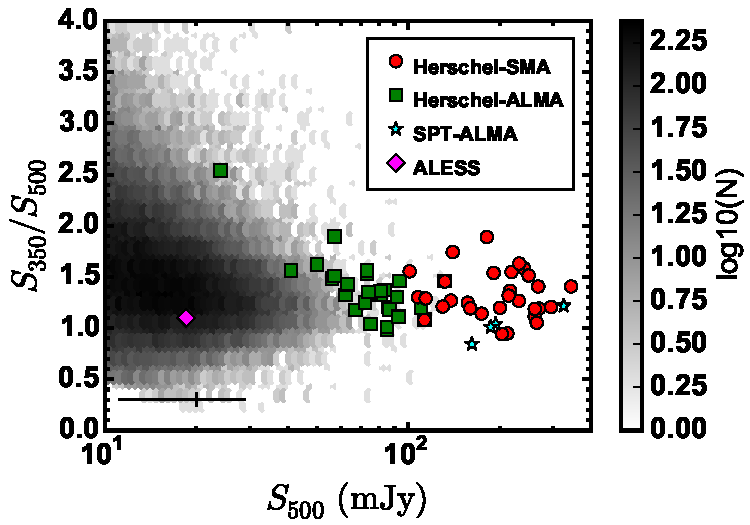
\includegraphics[width=\linewidth]{../Figures/spirecolflux.pdf}

\caption{ {\it Herschel}/SPIRE photometry of all galaxies in the H-ATLAS
phase~I catalog with S/N$ > 3$ at 250$\,\mu$m, 350$\,\mu$m, and 500$\,\mu$m
(grayscale).  The sample of HerMES sources in this paper are shown with green
squares (the ``ALMA sample'').  The very bright {\it Herschel} DSFGs from
\citet{Bussmann:2013lr} (the ``SMA sample'') are shown by red circles, and the
overall sample of candidate lensed {\it Herschel} DSFGs are highlighted by
yellow circles.  Lensed SMGs discovered by the SPT that have published lens
models are represented by cyan stars \citep{Hezaveh:2013fk}.  A magenta diamond
shows the location in this diagram of the stacked signal from ALESS DSFGs.
Representative error bars are shown in the lower left corner.  The ALMA sample
fills the gap in 500$\,\mu$m flux density space between SMA/SPT and ALESS
samples.} \label{fig:sample}

\end{figure}

In detail, two of the sources in the ALMA sample (HXMM01 and HXMM02) overlap
with the ``confirmed lensed'' sample in \citet{Wardlow:2013lr} as well as with
the SMA sample in \citet{Bussmann:2013lr}.  A further 8 appear in the
``Supplementary sample'' in \citet{Wardlow:2013lr}.  The remainder have
$S_{500} < 80\,$mJy and thus do not appear in \citet{Wardlow:2013lr}.

%Efforts are on-going to obtain a complete database of follow-up observations
%for our ALMA sample.  The present paper focuses on a
%subset of 30 candidates with superb existing follow-up observations (hereafter,
%we refer to this as the ``SMA subsample'').  These targets were initially
%selected on the basis of strong 1.2$\,$mm detections from the Max Planck
%Millimeter Bolometer (MAMBO) array \citep{Kreysa:1998uq} at the Institut de
%Radioastronomie Millim\'etrique (IRAM) 30$\,$m telescope (Dannerbauer et al. in
%prep.).  Subsequent follow-up efforts have now provided high-spatial resolution
%880$\, \mu$m imaging with the SMA, spectroscopic redshifts of the lensed SMGs
%obtained with GBT, CSO, CARMA, PdBI, and {\it Herschel} \citep[][Riechers et
%al., in prep.; Krips et al., in prep., George et al., in prep.]{Cox:2011fk,
%Harris:2012fr, Lupu:2012ly}, and spectroscopic redshifts to the lenses obtained
%with the MMT, Gemini-S, or WHT.  In addition, Keck-II Near InfraRed Camera 2
%(NIRC2) laser guide star adaptive optics (LGSAO) imaging has been obtained for
%nearly half of the candidate lensed SMG sample \citep[][Calanog et al., in
%prep.]{Wardlow:2013lr}.  These datasets provide the information needed to
%confirm the lensing hypothesis and begin analysis of the source and lens
%properties.  

Table~\ref{tab:position} provides reference data for the ALMA sample, including
centroid positions measured from the ALMA 870$\, \mu$m imaging (see
section~\ref{sec:almaobs}).

\subsection{ALMA Observations}\label{sec:almaobs}

ALMA data were obtained during Cycle~0 over a period from 2012 June to 2012
December (Program 2011.0.00539.S; PI: D. Riechers).  The observations were
carried out in good 870$\,\mu$m weather conditions which resulted in typical
system temperatures of $T_{\rm sys} \sim 130\,$K and phase fluctuations of $\sim
10\,$deg.  Each target was observed until an rms noise level of $\sigma \approx
0.2\,$mJy was achieved.  This typically required 10 minutes of on-source
integration time.  For the observations targeting the CDFS, Elais-S, and COSMOS
fields, the weather was of sufficient quality to reach $\sigma \approx
0.14\,$mJy.  The number of antennas used varied from 15 to 25.  The antennas
were configured with baseline lengths of 20$\,$m to 400$\,$m, providing a
synthesized beamsize of $\approx 0\farcs45$ FWHM while ensuring that no flux was
resolved out by the interferometer (since our targets all have size scales
smaller than $1-2 \arcsec$.  When possible, track-sharing of multiple
targets in a single track was used to optimize the {\it uv} coverage.

The quasars J0403$-$360, J2258$-$279, B0851$+$202, and J2258$-$279 were used
for bandpass and pointing calibration.  The quasars J0403$-$360, J0106$-$405,
J0519$-$454, J1008$+$063, and J0217$+017$ were used for amplitude and phase
gain calibration.  The following solar system objects were used for absolute
flux calibration: Callisto (CDFS targets), Neptune (XMM targets), Titan (COSMOS
targets) and Uranus (ADFS and XMM targets).  For HELAISS02, no solar system
object was observed.  Instead, J2258$-$279 was used for absolute flux
calibration, with the flux fixed according to a measurement made two days prior
to the observations of HELAISS02.

All observations were conducted with the correlator in ``Frequency Domain
Mode'', providing a total usable bandwidth of 7.5$\,$GHz with spectral windows
centered on 335.995$\,$GHz, 337.995$\,$GHz, 345.995$\,$GHz, 347.996$\,$GHz.  We
searched for evidence of serendipitous spectral lines but found none (typical
sensitivity is $\sigma \approx 8\,$mJy$\,$beam$^{-1}$ in 15$\,$km$\,$sec$^{-1}$
bins).

We used the Common Astronomy Software Applications (CASA, version 4.2.1)
package to investigate the quality of the reduced data provided by the North
American ALMA Science Center (NAASC).  Overall, the quality of the processed
data from the NAASC was very high.  We achieved a significant improvement in
the case of the ADFS and XMM targets by excluding datasets with moderate
$T_{\rm sys}$ and poor phase fluctuations.  For a handful of targets with peak
signal-to-noise ratio (S/N) greater than 20, we obtained a $\approx 10\%$
improvement in S/N by using the CASA {\sc selfcal} task to improve the phase
gain corrections.  Finally, we updated the absolute flux calibration to use the
Butler-JPL-Horizons 2012 solar system models.

For imaging, we used the CASA {\sc Clean} task with Briggs weighting and robust
= $+$0.5 to achieve an optimal balance between sensitivity and spatial
resolution.  We selected the multi-frequency synthesis option to optimize {\it
uv} coverage.  We designed custom masks for each target in CASA to ensure that
only regions with high S/N were considered during the cleaning process.

Figure~\ref{fig:imaging} presents our ALMA images (colorscale) in comparison to
the {\it Herschel} SPIRE images (black-white contours) originally used to
select the targets and noted in each panel as either 250$\,\mu$m or
350$\,\mu$m.  Each panel is centered on the phase center of the ALMA
observations of that target and a white circle traces the FWHM of the primary
beam of an ALMA 12$\,$m antenna at 870$\,\mu$m.  A white dashed box represents
the region of each image that is shown in greater detail in
Figure~\ref{fig:uvmodels}.

In most targets, the peak of the SPIRE map is spatially coincident with the
location of the ALMA sources.  In one case where two ALMA sources are separated
by $\approx 10\arcsec$ (HADFS08), the elongation in the SPIRE 250$\,\mu$m map is
consistent with the angular separation of the two ALMA counterparts.
Otherwise, the SPIRE imaging is consistent with a single component located at
the centroid of the ALMA sources.  This result is not a surprise, given the
typical angular separation of the ALMA sources ($\lesssim 5\arcsec$) and the
FWHM of the SPIRE beam at 250$\,\mu$m (18.1$\arcsec$). 

\subsection{Gemini-South Imaging}\label{sec:geminiobs}

Optical imaging observations using the Gemini Multi-Object Spectrograph-South
\citep[GMOS-S;][]{Hook:2004qy} were conducted in queue mode during the 2013B
semester as part of program GS-2013B-Q-77 (PI: R.~S.~Bussmann).  The goal of the
program is to use shallow $u$, $g$, $r$, $i$, and $z$ imaging to identify
structure at $z<1$ and determine which of the ALMA sources are affected by
gravitational lensing.  Nearly half of the ALMA sources lie in regions with
existing deep optical imaging thanks to the extensive HerMES multi-wavelength
dataset --- these were excluded from our Gemini-S program.  The remaining
targets are: HADFS03, HADFS08, HADFS09, HADFS10, HADFS02, HADFS04, HADFS01, HADFS11,
HELAISS02, HXMM11, HXMM12, HXMM22, HXMM07, HXMM30, and HXMM04.  Each of these
targets were observed for a total of 9$\,$minutes of on-source integration time
in each of $u$, $g$, $r$, $i$, and $z$.  The observations were obtained during
dark time in with adequate seeing conditions (image quality $ = 85\% \approx
1.1\arcsec$.

The data were reduced using the standard {\sc IRAF} Gemini GMOS reduction
routines, following the standard GMOS-S reduction steps in the example taken
from the Gemini observatory webpage
\footnote{http://www.gemini.edu/sciops/data-and-results/processing-software/getting-started\#gmos}.

We used the Sloan Digital Sky Survey (SDSS) or the 2 Micron All Sky Survey
(2MASS) to align the Gemini-S images to a common astrometric frame of
reference.  This imposes an rms uncertainty in the absolute astrometry of
$0\farcs2$ and $0\farcs4$ for SDSS and 2MASS, respectively.  The
astrometrically calibrated Gemini-S images served as the basis for aligning
higher resolution, smaller field-of-view imaging from {\it HST} or Keck (when
available) that were originally presented in \citet{Calanog:2014lr}.

%\clearpage
\LongTables
\begin{deluxetable*}{llccccccc}[!tbp]
%\rotate
%\resizebox{\textwidth}{!}{%
\tabletypesize{\scriptsize}
\tablecolumns{9}
%\tablewidth{7.5in}
\tablecaption{Observed positions and flux densities of ALMA sources. Positional
For each {\it Herschel} source, we give the fiducial flux density in all SPIRE
bands (see main text) Observed positions and flux densities of ALMA sources. Positional
uncertainties (for unlensed sources) range from $\approx 0\farcs005$ for
well-detected sources to $\approx 0\farcs15$ for the faintest soures in our
sample.  Uncertainties in flux density do not include the absolute calibration
uncertainty of $\approx 10\%$. Quoted uncertainties in {\it Herschel}
photometry are dominated by confusion noise.}
%Definition of lens grades: \\
%Reference key: G05 = \citet{Gladders:2005qy}; B06 = \citet{Borys:2006lr}; N10 =
%\citet{Negrello:2010fk}; S11 = \citet{2011ApJ...733...29S}; F11 = \citet{2011ApJ...726L..22F}; C11 =
%\citet{Cox:2011fk}; H12 = \citet{Harris:2012fr}; B12 = \citet{Bussmann:2012lr};
%L12 = \citet{Lupu:2012ly}; W13 = \citet{Wardlow:2013lr}; I13 =
%\citet{Ivison:2013fk}; G13 = George et al. (in prep.); R13 = Riechers et al.
%(in prep.); K13 = Krips et al. (in prep.); L13 = Lupu et al. (in prep.); H13 = Harris et al. (in prep.).}
\tablehead{
\colhead{} & 
\colhead{} & 
\colhead{RA$_{870}$} &
\colhead{Dec$_{870}$} &
\colhead{$S_{250}$} &
\colhead{$S_{350}$} &
\colhead{$S_{500}$} &
\colhead{$S_{870}$} &
\colhead{Lens}
\\
\colhead{IAU address\tablenotemark{a}} & 
\colhead{Short name} & 
\colhead{(J2000)} &
\colhead{(J2000)} &
\colhead{(mJy)} &
\colhead{(mJy)} &
\colhead{(mJy)} &
\colhead{(mJy)} &
\colhead{grade\tablenotemark{b}}
}
\startdata
J003823.6$-$433707            & HELAISS02  & 00:38:23.587 & $-$43:37:04.15  & $ 115 \pm  6$ & $ 124 \pm  6$ & $ 108 \pm  6$   &    $20.11\pm 0.45$  & --- \\
---                           & Source0    & 00:38:23.762 & $-$43:37:06.10  & --- & --- & ---                                 &    $ 9.22\pm 0.17$  & C   \\
---                           & Source1    & 00:38:23.482 & $-$43:37:05.56  & --- & --- & ---                                 &    $ 4.34\pm 0.16$  & C   \\
---                           & Source2    & 00:38:23.313 & $-$43:36:58.97  & --- & --- & ---                                 &    $ 4.16\pm 0.32$  & C   \\
---                           & Source3    & 00:38:23.803 & $-$43:37:10.46  & --- & --- & ---                                 &    $ 2.40\pm 0.19$  & C   \\
J021830.5$-$053124            & HXMM02     & 02:18:30.673 & $-$05:31:31.75  & $  78 \pm  7$ & $ 122 \pm  8$ & $  99 \pm  7$   &    $63.33\pm 0.58$  & A   \\
J021841.5$-$035002            & HXMM31     & 02:18:41.613 & $-$03:50:03.70  & $ 102 \pm  6$ & $  94 \pm  6$ & $  65 \pm  6$   &    $10.80\pm 0.46$  & --- \\
---                           & Source0    & 02:18:41.520 & $-$03:50:04.72  & --- & --- & ---                                 &    $ 6.79\pm 0.37$  & C   \\
---                           & Source1    & 02:18:41.700 & $-$03:50:02.57  & --- & --- & ---                                 &    $ 4.01\pm 0.26$  & C   \\
J021853.1$-$063325            & HXMM29     & 02:18:53.111 & $-$06:33:24.65  & $  97 \pm  6$ & $ 102 \pm  6$ & $  78 \pm  6$   &    $ 7.28\pm 0.45$  & --- \\
---                           & Source0    & 02:18:53.118 & $-$06:33:24.19  & --- & --- & ---                                 &    $ 5.46\pm 0.30$  & C   \\
---                           & Source1    & 02:18:53.095 & $-$06:33:25.21  & --- & --- & ---                                 &    $ 1.82\pm 0.38$  & C   \\
J021918.4$-$031051            & HXMM07     & 02:19:18.417 & $-$03:10:51.35  & $  89 \pm  7$ & $ 107 \pm  8$ & $  85 \pm  7$   &    $29.16\pm 0.58$  & A   \\
J021942.7$-$052436            & HXMM20     & 02:19:42.783 & $-$05:24:34.84  & $  72 \pm  6$ & $  85 \pm  6$ & $  66 \pm  6$   &    $17.49\pm 0.74$  & --- \\
---                           & Source0    & 02:19:42.629 & $-$05:24:37.11  & --- & --- & ---                                 &    $ 7.15\pm 0.44$  & X   \\
---                           & Source1    & 02:19:42.838 & $-$05:24:35.11  & --- & --- & ---                                 &    $ 3.52\pm 0.41$  & X   \\
---                           & Source2    & 02:19:42.769 & $-$05:24:36.48  & --- & --- & ---                                 &    $ 3.42\pm 0.26$  & X   \\
---                           & Source3    & 02:19:42.682 & $-$05:24:36.82  & --- & --- & ---                                 &    $ 2.46\pm 0.47$  & X   \\
---                           & Source4    & 02:19:42.955 & $-$05:24:32.22  & --- & --- & ---                                 &    $ 0.94\pm 0.18$  & X   \\
J022016.5$-$060143            & HXMM01     & 02:20:16.609 & $-$06:01:43.18  & $ 179 \pm  7$ & $ 188 \pm  8$ & $ 134 \pm  7$   &    $29.56\pm 0.46$  & --- \\
---                           & Source0    & 02:20:16.648 & $-$06:01:41.93  & --- & --- & ---                                 &    $16.13\pm 0.31$  & C   \\
---                           & Source1    & 02:20:16.571 & $-$06:01:44.56  & --- & --- & ---                                 &    $11.56\pm 0.32$  & C   \\
---                           & Source2    & 02:20:16.609 & $-$06:01:40.72  & --- & --- & ---                                 &    $ 1.87\pm 0.26$  & C   \\
J022021.7$-$015328            & HXMM04     & 02:20:21.756 & $-$01:53:30.92  & $ 162 \pm  7$ & $ 157 \pm  8$ & $ 125 \pm 11$   &    $20.03\pm 0.47$  & C   \\
J022029.2$-$064845            & HXMM09     & 02:20:29.140 & $-$06:48:46.49  & $ 129 \pm  7$ & $ 118 \pm  8$ & $  85 \pm  7$   &    $15.30\pm 0.36$  & --- \\
---                           & Source0    & 02:20:29.195 & $-$06:48:48.02  & --- & --- & ---                                 &    $ 8.93\pm 0.30$  & C   \\
---                           & Source1    & 02:20:29.079 & $-$06:48:44.86  & --- & --- & ---                                 &    $ 6.37\pm 0.19$  & C   \\
J022135.1$-$062617            & HXMM03     & 02:21:34.891 & $-$06:26:17.87  & $ 114 \pm  7$ & $ 134 \pm  8$ & $ 116 \pm  7$   &    $22.65\pm 0.36$  & --- \\
---                           & Source1    & 02:21:35.124 & $-$06:26:16.62  & --- & --- & ---                                 &    $18.42\pm 0.36$  & C   \\
---                           & Source2    & 02:21:35.132 & $-$06:26:18.02  & --- & --- & ---                                 &    $ 2.19\pm 0.20$  & C   \\
---                           & Source0    & 02:21:35.136 & $-$06:26:17.28  & --- & --- & ---                                 &    $ 2.03\pm 0.18$  & C   \\
J022201.6$-$033340            & HXMM11     & 02:22:01.616 & $-$03:33:41.40  & $ 101 \pm  7$ & $ 104 \pm  8$ & $  73 \pm  7$   &    $11.72\pm 0.49$  & --- \\
---                           & Source0    & 02:22:01.592 & $-$03:33:39.42  & --- & --- & ---                                 &    $ 8.17\pm 0.32$  & C   \\
---                           & Source1    & 02:22:01.629 & $-$03:33:43.58  & --- & --- & ---                                 &    $ 3.54\pm 0.36$  & C   \\
J022205.4$-$070728            & HXMM23     & 02:22:05.362 & $-$07:07:28.10  & $ 128 \pm  6$ & $ 105 \pm  6$ & $  68 \pm  6$   &    $ 2.93\pm 0.15$  & X   \\
J022250.5$-$032410            & HXMM22     & 02:22:50.573 & $-$03:24:12.35  & $ 101 \pm  6$ & $  85 \pm  6$ & $  61 \pm  6$   &    $10.19\pm 0.28$  & C   \\
J022547.8$-$041750            & HXMM05    & 02:25:47.942 & $-$04:17:50.80  & $ 103 \pm  7$ & $ 118 \pm  8$ & $  97 \pm  7$   &    $17.96\pm 0.43$  & C  \\
J022944.7$-$034110            & HXMM30     & 02:29:44.740 & $-$03:41:09.57  & $  86 \pm  6$ & $  97 \pm  6$ & $  75 \pm  6$   &    $22.76\pm 0.28$  & A   \\
J023006.0$-$034152            & HXMM12     & 02:30:05.950 & $-$03:41:53.07  & $  98 \pm  7$ & $ 106 \pm  8$ & $  82 \pm  7$   &    $15.56\pm 0.37$  & C   \\
J032752.0$-$290908            & HECDFS12   & 03:27:52.011 & $-$29:09:10.40  & $  61 \pm  7$ & $  82 \pm  6$ & $  81 \pm  6$   &    $38.78\pm 0.56$  & --- \\
---                           & Source0    & 03:27:52.002 & $-$29:09:12.07  & --- & --- & ---                                 &    $16.76\pm 0.51$  & A   \\
---                           & Source1    & 03:27:52.002 & $-$29:09:09.65  & --- & --- & ---                                 &    $14.55\pm 0.22$  & C   \\
---                           & Source2    & 03:27:52.025 & $-$29:09:12.14  & --- & --- & ---                                 &    $ 7.47\pm 0.14$  & X   \\
J033210.8$-$270535            & HECDFS04   & 03:32:10.840 & $-$27:05:34.18  & $  56 \pm  6$ & $  61 \pm  6$ & $  55 \pm  6$   &    $14.57\pm 0.26$  & --- \\
---                           & Source0    & 03:32:10.905 & $-$27:05:32.87  & --- & --- & ---                                 &    $11.91\pm 0.24$  & C   \\
---                           & Source1    & 03:32:10.729 & $-$27:05:36.22  & --- & --- & ---                                 &    $ 2.66\pm 0.11$  & C   \\
J033317.9$-$280907            & HECDFS13   & 03:33:18.017 & $-$28:09:07.52  & $  95 \pm  6$ & $  89 \pm  6$ & $  63 \pm  6$   &    $15.36\pm 0.27$  & --- \\
---                           & Source0    & 03:33:18.006 & $-$28:09:07.55  & --- & --- & ---                                 &    $10.11\pm 1.30$  & X   \\
---                           & Source1    & 03:33:18.032 & $-$28:09:07.39  & --- & --- & ---                                 &    $ 5.25\pm 1.37$  & X   \\
J043340.5$-$540337            & HADFS04    & 04:33:40.450 & $-$54:03:39.51  & $  74 \pm  6$ & $  93 \pm  6$ & $  84 \pm  6$   &    $18.12\pm 0.44$  & --- \\
---                           & Source0    & 04:33:40.455 & $-$54:03:40.29  & --- & --- & ---                                 &    $ 9.25\pm 0.30$  & C   \\
---                           & Source1    & 04:33:40.501 & $-$54:03:40.05  & --- & --- & ---                                 &    $ 6.09\pm 0.33$  & C   \\
---                           & Source2    & 04:33:40.472 & $-$54:03:38.33  & --- & --- & ---                                 &    $ 2.78\pm 0.19$  & C   \\
J043619.3$-$552425            & HADFS02    & 04:36:19.702 & $-$55:24:25.01  & $ 102 \pm  6$ & $  97 \pm  6$ & $  81 \pm  5$   &    $16.79\pm 0.40$  & --- \\
---                           & Source0    & 04:36:19.706 & $-$55:24:24.41  & --- & --- & ---                                 &    $ 7.81\pm 0.47$  & X   \\
---                           & Source1    & 04:36:19.698 & $-$55:24:25.27  & --- & --- & ---                                 &    $ 8.99\pm 0.58$  & X   \\
J043829.7$-$541831            & HADFS11    & 04:38:30.883 & $-$54:18:29.38  & $  19 \pm  6$ & $  39 \pm  5$ & $  52 \pm  6$   &    $28.47\pm 0.64$  & --- \\
---                           & Source0    & 04:38:30.780 & $-$54:18:31.79  & --- & --- & ---                                 &    $21.19\pm 0.51$  & C   \\
---                           & Source1    & 04:38:30.970 & $-$54:18:26.60  & --- & --- & ---                                 &    $ 7.28\pm 0.30$  & C   \\
J044103.8$-$531240            & HADFS10    & 04:41:03.942 & $-$53:12:41.01  & $  47 \pm  6$ & $  58 \pm  6$ & $  58 \pm  6$   &    $17.44\pm 0.39$  & --- \\
---                           & Source0    & 04:41:03.866 & $-$53:12:41.33  & --- & --- & ---                                 &    $ 9.61\pm 0.25$  & X   \\
---                           & Source1    & 04:41:04.000 & $-$53:12:40.10  & --- & --- & ---                                 &    $ 4.59\pm 0.23$  & X   \\
---                           & Source2    & 04:41:03.912 & $-$53:12:42.09  & --- & --- & ---                                 &    $ 3.24\pm 0.19$  & X   \\
J044153.9$-$540350            & HADFS01    & 04:41:53.880 & $-$54:03:53.48  & $  76 \pm  6$ & $ 100 \pm  6$ & $  94 \pm  6$   &    $32.79\pm 0.47$  & A   \\
J044946.9$-$525424            & HADFS09    & 04:49:46.448 & $-$52:54:26.95  & $  98 \pm  6$ & $ 102 \pm  6$ & $  72 \pm  6$   &    $15.52\pm 0.59$  & --- \\
---                           & Source0    & 04:49:46.603 & $-$52:54:23.66  & --- & --- & ---                                 &    $ 8.24\pm 0.26$  & X   \\
---                           & Source1    & 04:49:46.301 & $-$52:54:30.26  & --- & --- & ---                                 &    $ 4.86\pm 0.34$  & X   \\
---                           & Source2    & 04:49:46.280 & $-$52:54:26.06  & --- & --- & ---                                 &    $ 2.42\pm 0.35$  & X   \\
J045026.5$-$524127            & HADFS08    & 04:50:27.453 & $-$52:41:25.41  & $ 142 \pm  6$ & $ 133 \pm  6$ & $  90 \pm  6$   &    $14.18\pm 0.50$  & --- \\
---                           & Source0    & 04:50:27.092 & $-$52:41:25.62  & --- & --- & ---                                 &    $ 6.17\pm 0.28$  & C   \\
---                           & Source1    & 04:50:27.806 & $-$52:41:25.10  & --- & --- & ---                                 &    $ 8.01\pm 0.43$  & C   \\
J045057.5$-$531654            & HADFS03    & 04:50:57.715 & $-$53:16:54.42  & $ 119 \pm  6$ & $ 102 \pm  6$ & $  63 \pm  6$   &    $11.50\pm 0.39$  & --- \\
---                           & Source0    & 04:50:57.610 & $-$53:16:55.09  & --- & --- & ---                                 &    $ 7.12\pm 0.22$  & C   \\
---                           & Source1    & 04:50:57.805 & $-$53:16:56.96  & --- & --- & ---                                 &    $ 2.12\pm 0.14$  & C   \\
---                           & Source2    & 04:50:57.741 & $-$53:16:54.54  & --- & --- & ---                                 &    $ 2.27\pm 0.26$  & C   \\
J100056.6$+$022014            & HCOSMOS02  & 10:00:57.180 & $+$02:20:12.70  & $  70 \pm  6$ & $  85 \pm  6$ & $  71 \pm  6$   &    $14.61\pm 0.66$  & --- \\
---                           & Source0    & 10:00:56.946 & $+$02:20:17.35  & --- & --- & ---                                 &    $ 5.26\pm 0.26$  & X   \\
---                           & Source1    & 10:00:57.565 & $+$02:20:11.26  & --- & --- & ---                                 &    $ 3.77\pm 0.32$  & X   \\
---                           & Source2    & 10:00:56.855 & $+$02:20:08.93  & --- & --- & ---                                 &    $ 1.69\pm 0.25$  & X   \\
---                           & Source3    & 10:00:57.274 & $+$02:20:12.66  & --- & --- & ---                                 &    $ 1.66\pm 0.21$  & X   \\
---                           & Source4    & 10:00:57.400 & $+$02:20:10.83  & --- & --- & ---                                 &    $ 2.23\pm 0.41$  & X   \\
J100144.1$+$025712            & HCOSMOS01  & 10:01:44.182 & $+$02:57:12.47  & $  86 \pm  6$ & $  96 \pm  6$ & $  71 \pm  6$   &    $15.35\pm 0.25$  & A   \\
\enddata
\label{tab:position}
%\tnt{a}{Multiple lens redshifts have been measured for these targets.  The redshift uncertainty is 0.001 in all cases.}
\tablenotetext{a}{IAU name = 1HerMES S250 + IAU address}
\tablenotetext{b}{A = strongly lensed, C = weakly lensed, X = unlensed.  Discussion of lens grades are given in Section~\ref{sec:objectbyobject}.}
%\tablenotetext{c}{WHT/ACAM?}
%\tablenotetext{d}{\citet{Bussmann:2012lr}}
% 
%\tablenotetext{a}{\citet{Lupu:2012ly}}
%\tablenotetext{b}{\citet{Harris:2012fr}}
%\tablenotetext{c}{\citet{2011ApJ...726L..22F}}
%\tablenotetext{d}{Riechers et al., in prep.}
%\tablenotetext{e}{Krips et al., in prep.}
%\tablenotetext{f}{\citet{Cox:2011fk}}
%\tablenotetext{g}{George et al., in prep.}
%%\tablenotetext{h}{\citep{Wardlow:2013lr}}
\end{deluxetable*}


\begin{figure*}[!tbp] 
    \begin{centering}
%\epsscale{1.00} 
%\includegraphics[width=\textwidth]{cutouts_dec17.png}
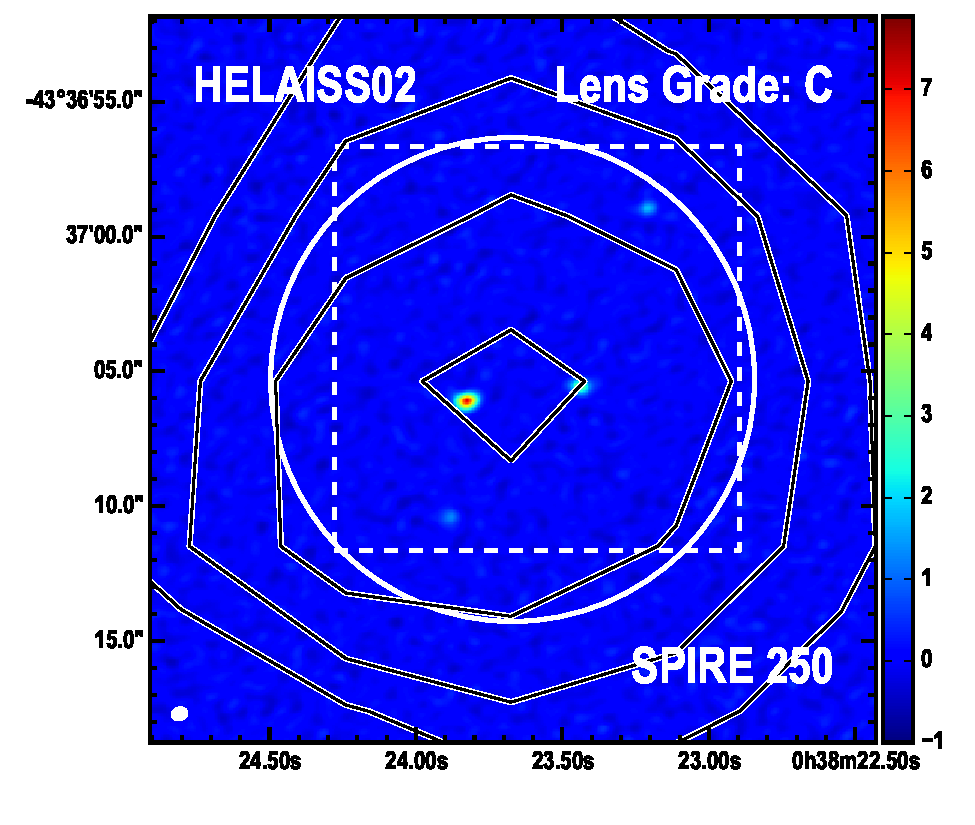
\includegraphics[width=0.331\textwidth]{../Figures/overlays/HELAISS02_870_250.pdf}
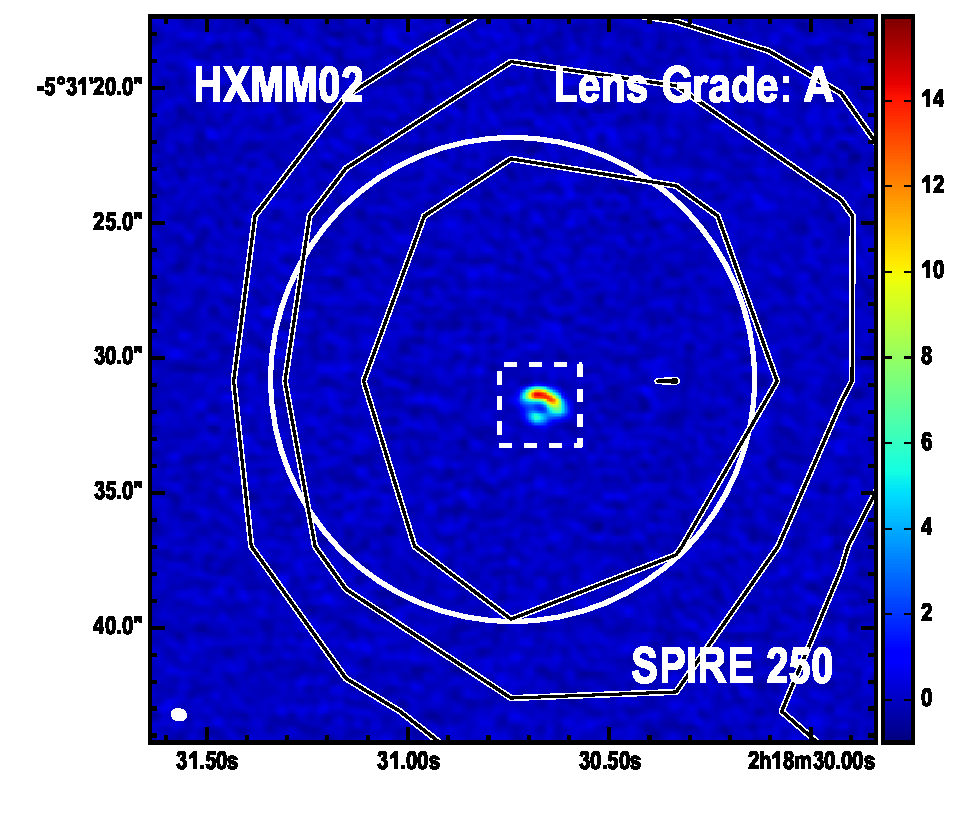
\includegraphics[width=0.331\textwidth]{../Figures/overlays/HXMM02_870_250.pdf}
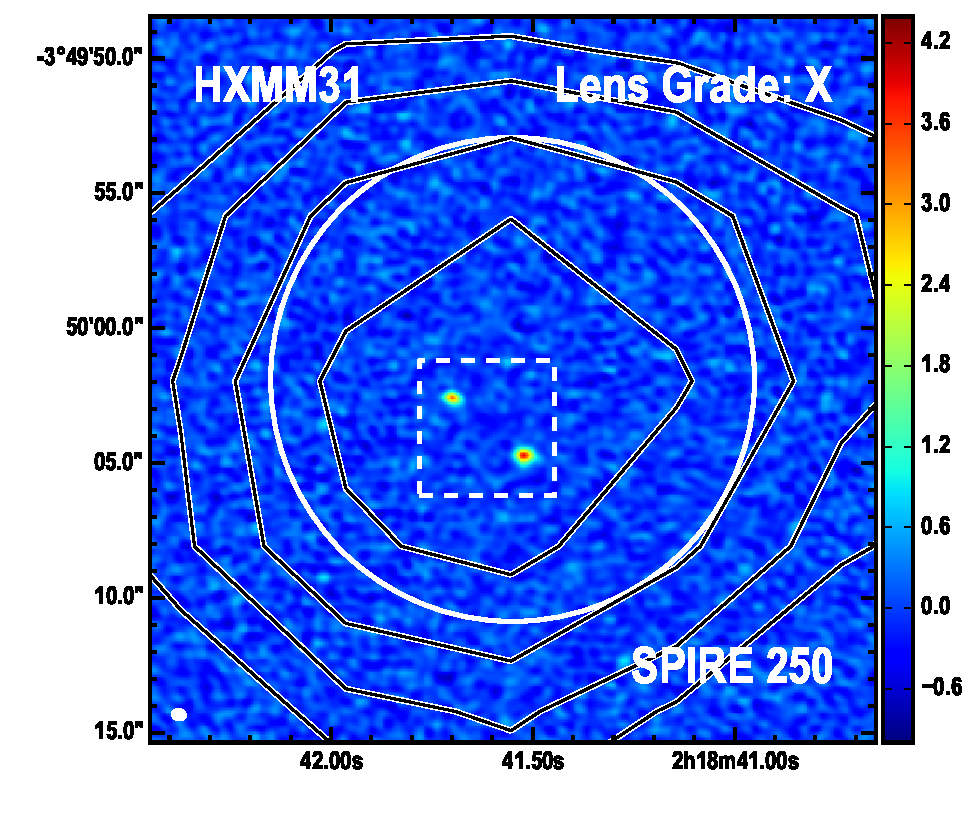
\includegraphics[width=0.331\textwidth]{../Figures/overlays/HXMM31_870_250.pdf}
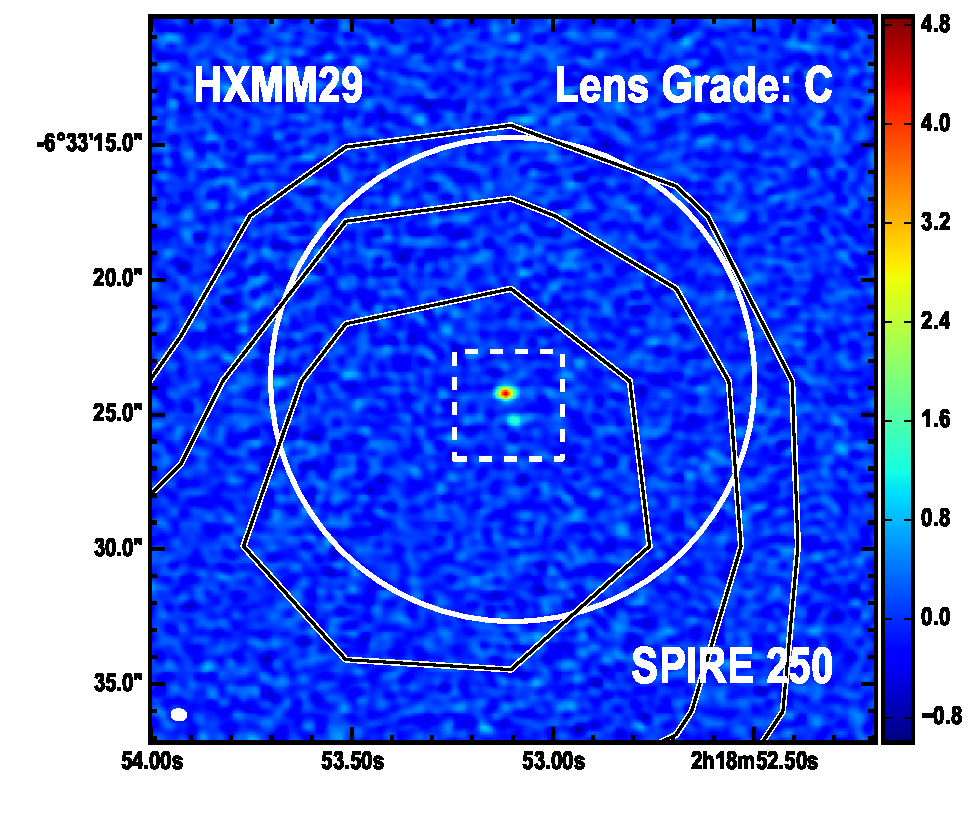
\includegraphics[width=0.331\textwidth]{../Figures/overlays/HXMM29_870_250.pdf}
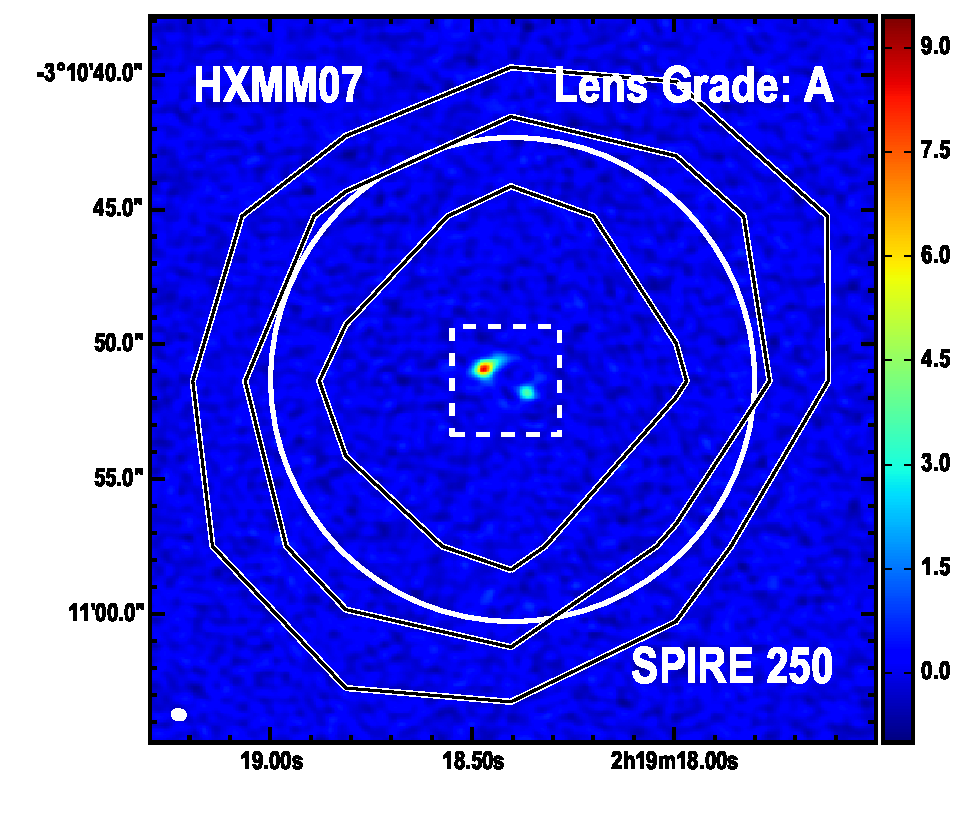
\includegraphics[width=0.331\textwidth]{../Figures/overlays/HXMM07_870_250.pdf}
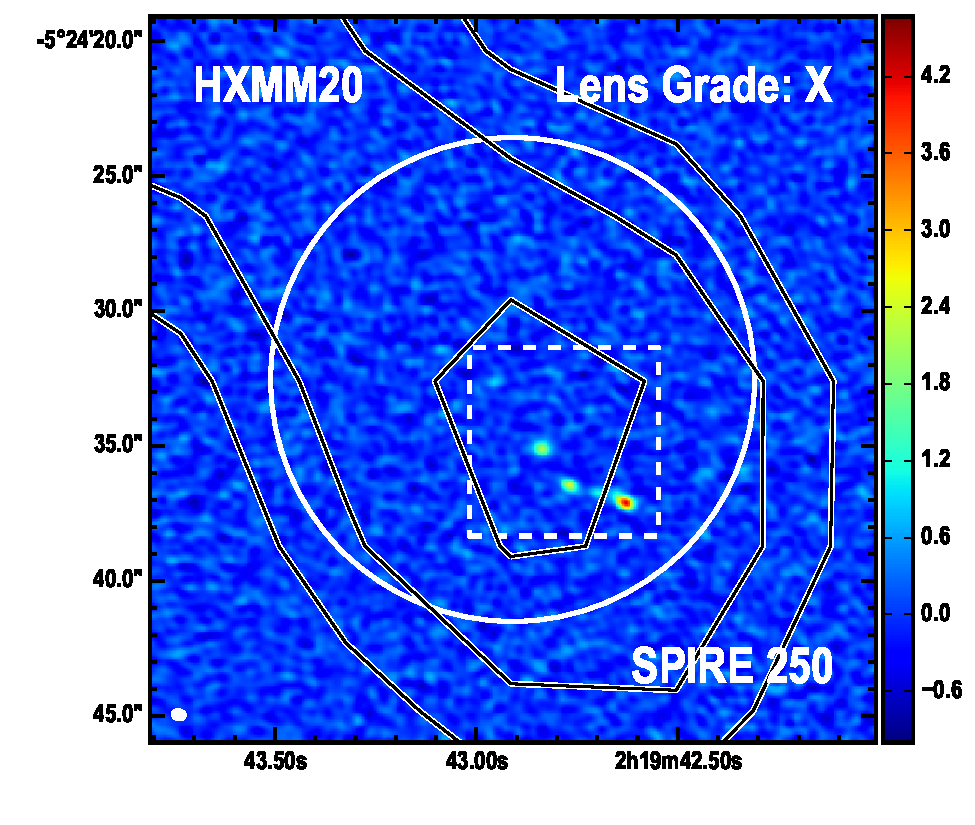
\includegraphics[width=0.331\textwidth]{../Figures/overlays/HXMM20_870_250.pdf}
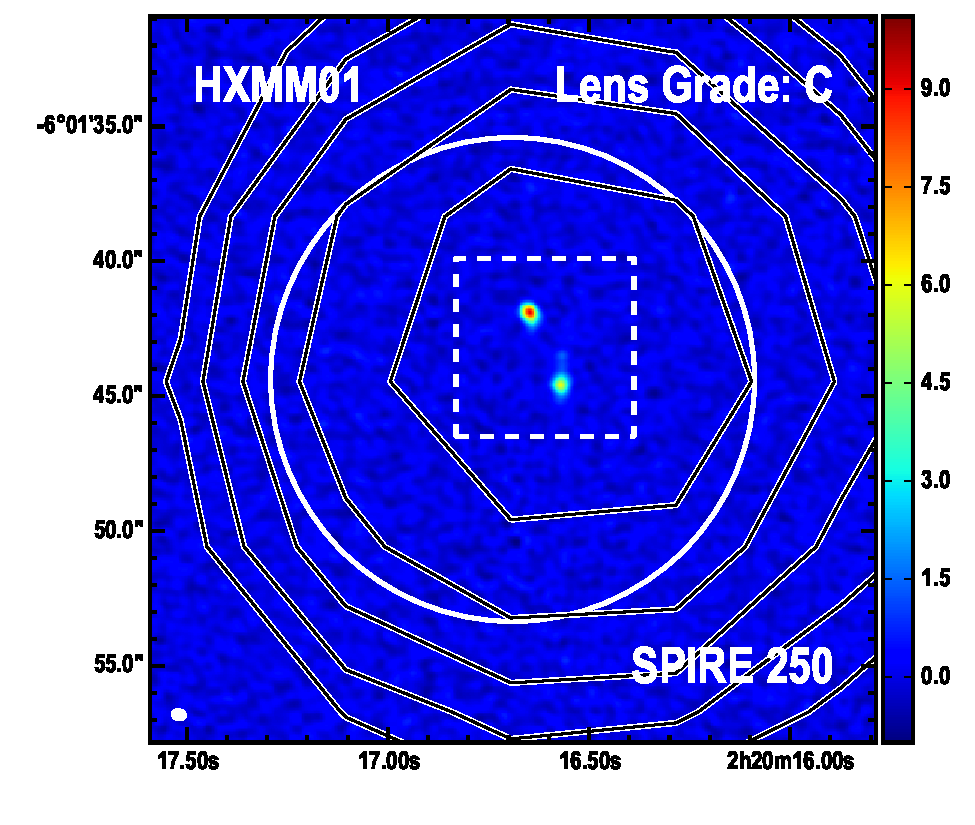
\includegraphics[width=0.331\textwidth]{../Figures/overlays/HXMM01_870_250.pdf}
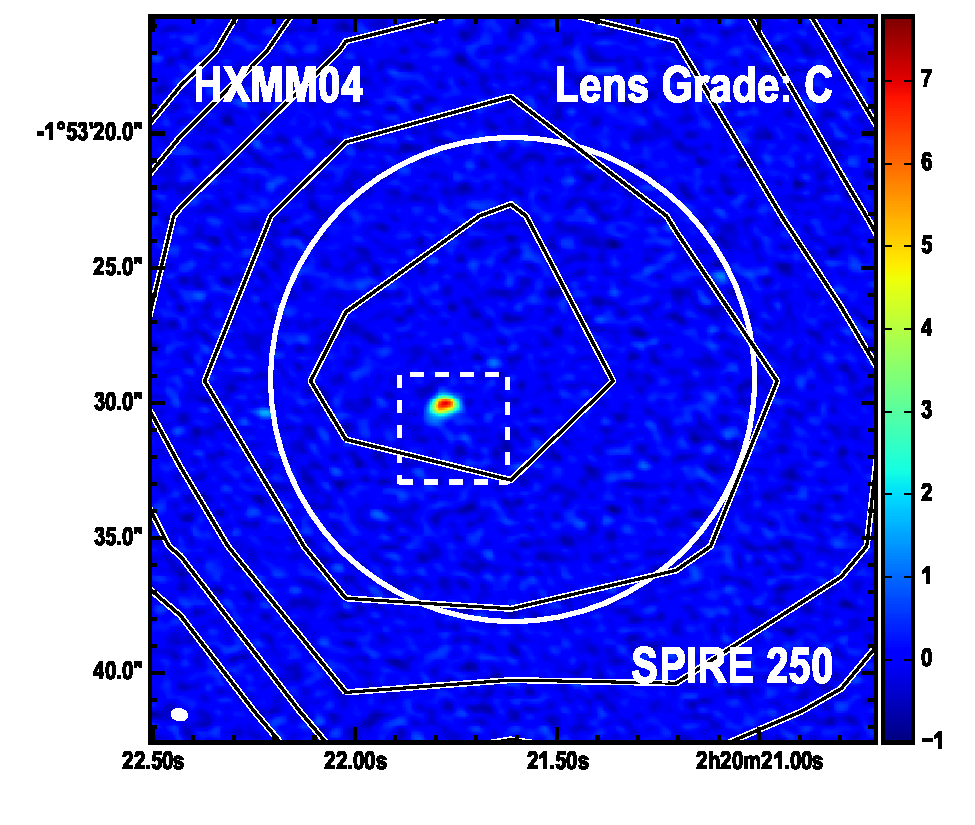
\includegraphics[width=0.331\textwidth]{../Figures/overlays/HXMM04_870_250.pdf}
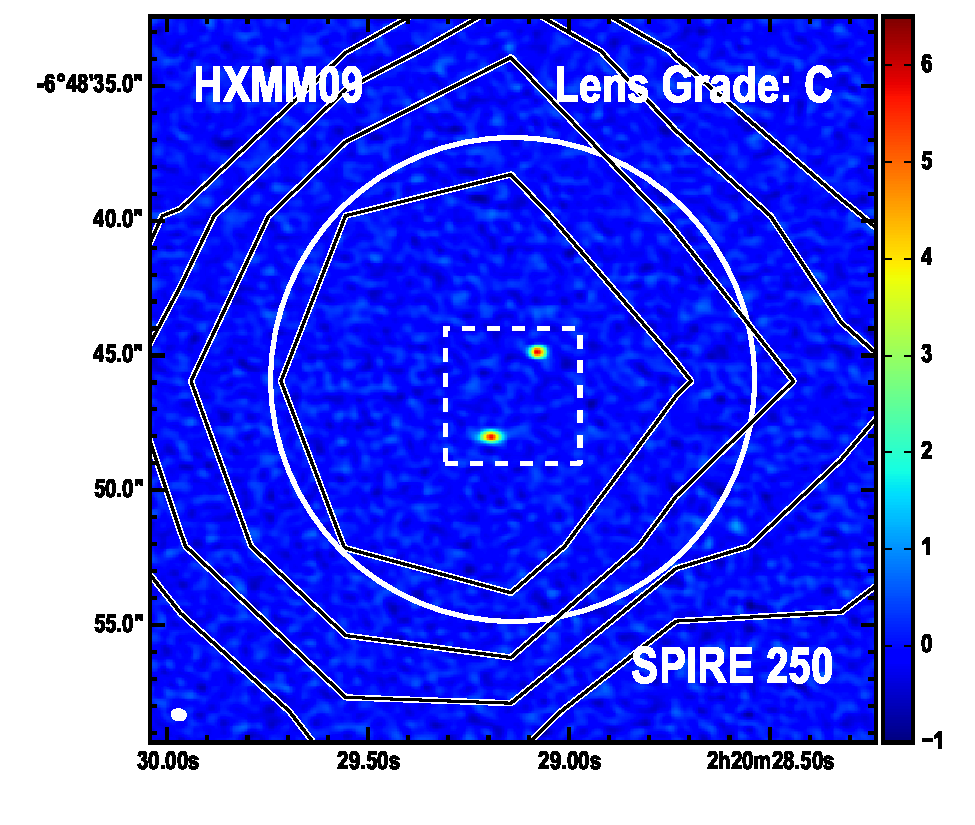
\includegraphics[width=0.331\textwidth]{../Figures/overlays/HXMM09_870_250.pdf}
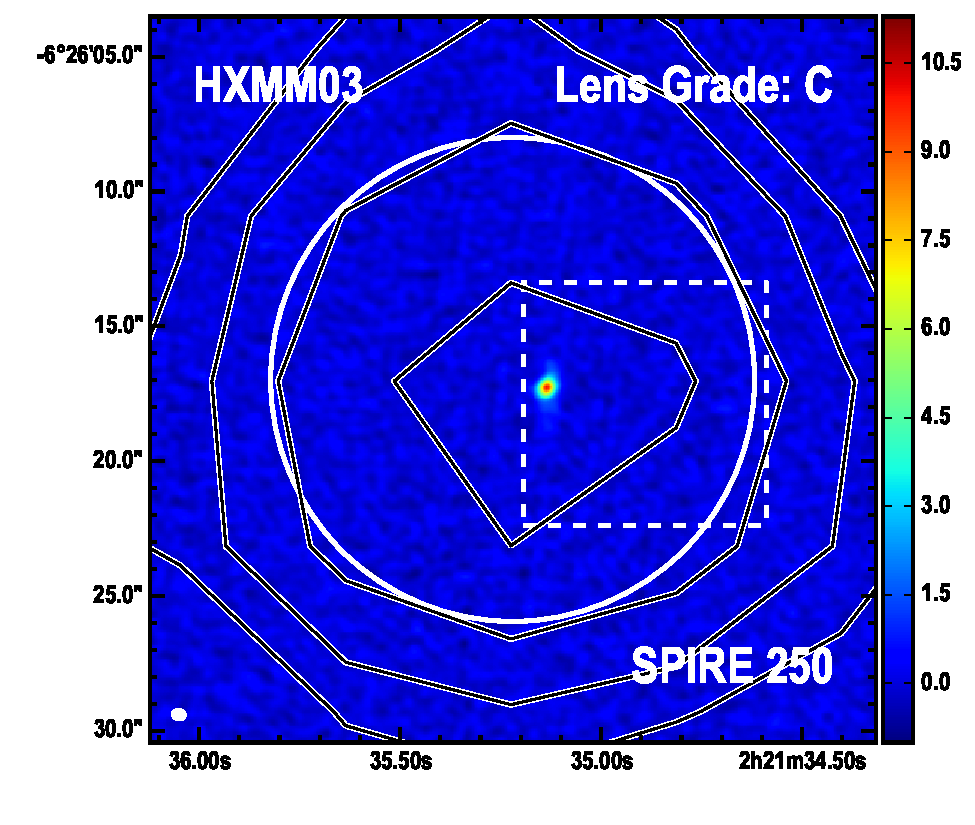
\includegraphics[width=0.331\textwidth]{../Figures/overlays/HXMM03_870_250.pdf}
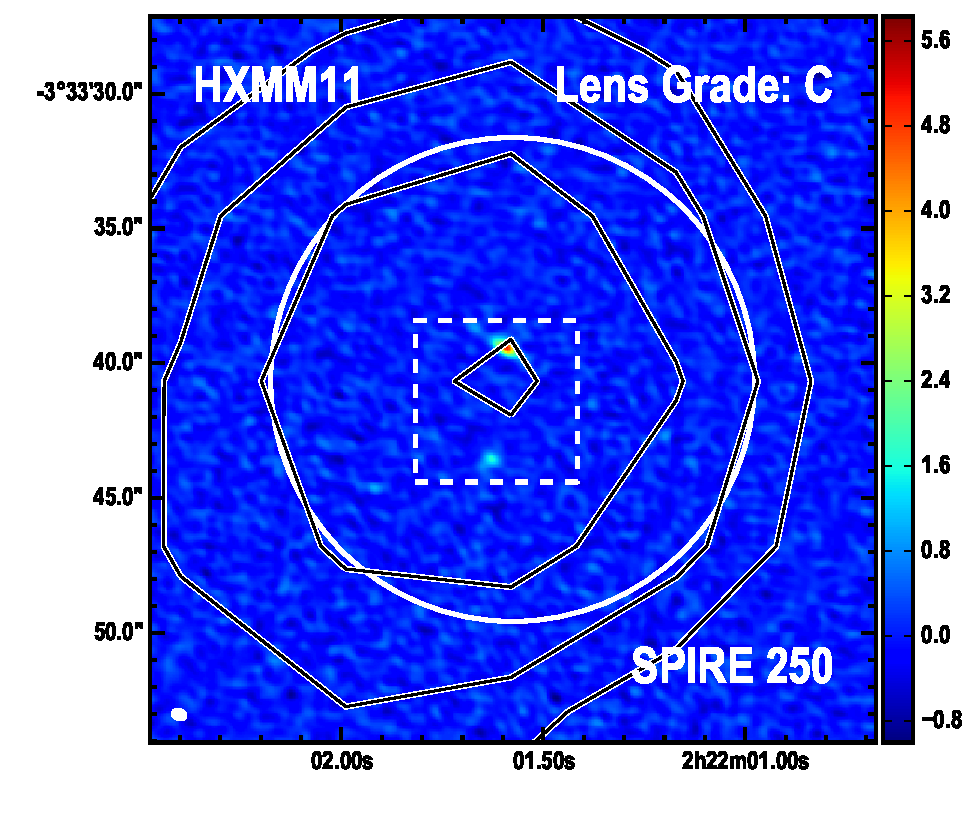
\includegraphics[width=0.331\textwidth]{../Figures/overlays/HXMM11_870_250.pdf}
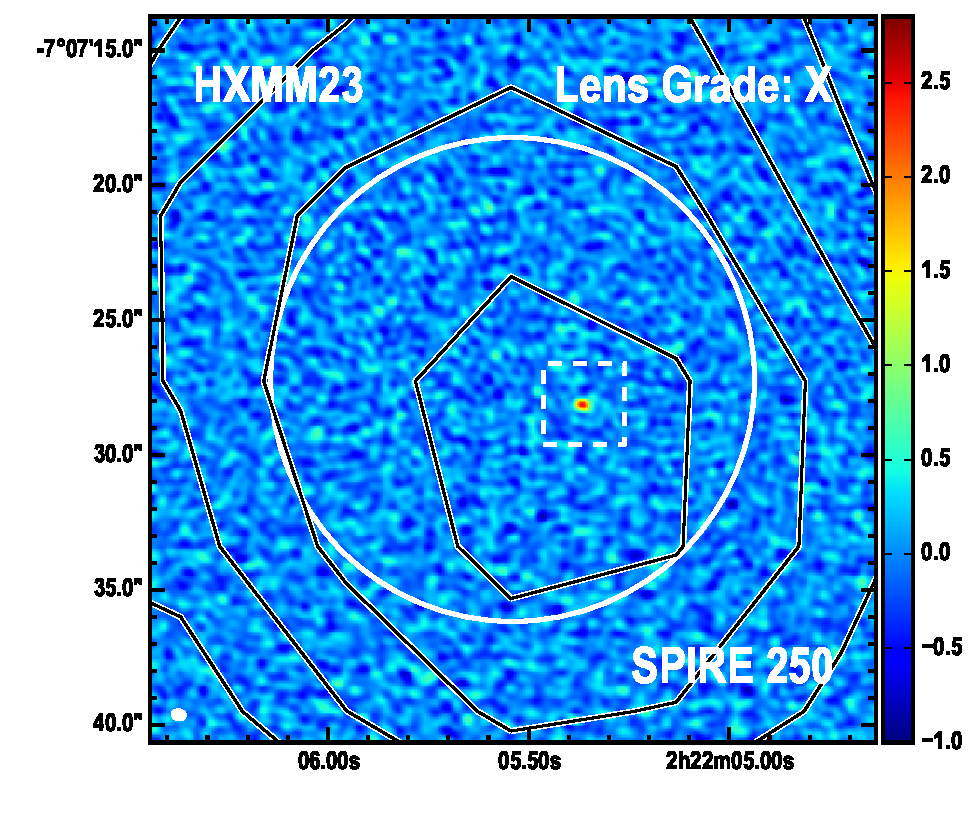
\includegraphics[width=0.331\textwidth]{../Figures/overlays/HXMM23_870_250.pdf}
\end{centering}

\caption{ ALMA 870$\mu$m images (color scale, units of mJy/beam) of HerMES
DSFGs.  Contours (black and white) trace 250$\,\mu$m emission from {\it
Herschel}.  The FWHM size of the ALMA synthesized beam is shown in the lower
left corner of each panel.  A solid white circle shows the FWHM size of the
primary beam.  Dashed squares identify the regions of each image that are shown
in greater detail in Figure~\ref{fig:uvmodels}.  \label{fig:imaging}}
\addtocounter{figure}{-1}

\end{figure*}

\begin{figure*}[!tbp] 
    \begin{centering}
%\epsscale{1.00} 
%\includegraphics[width=\textwidth]{cutouts_dec17.png}
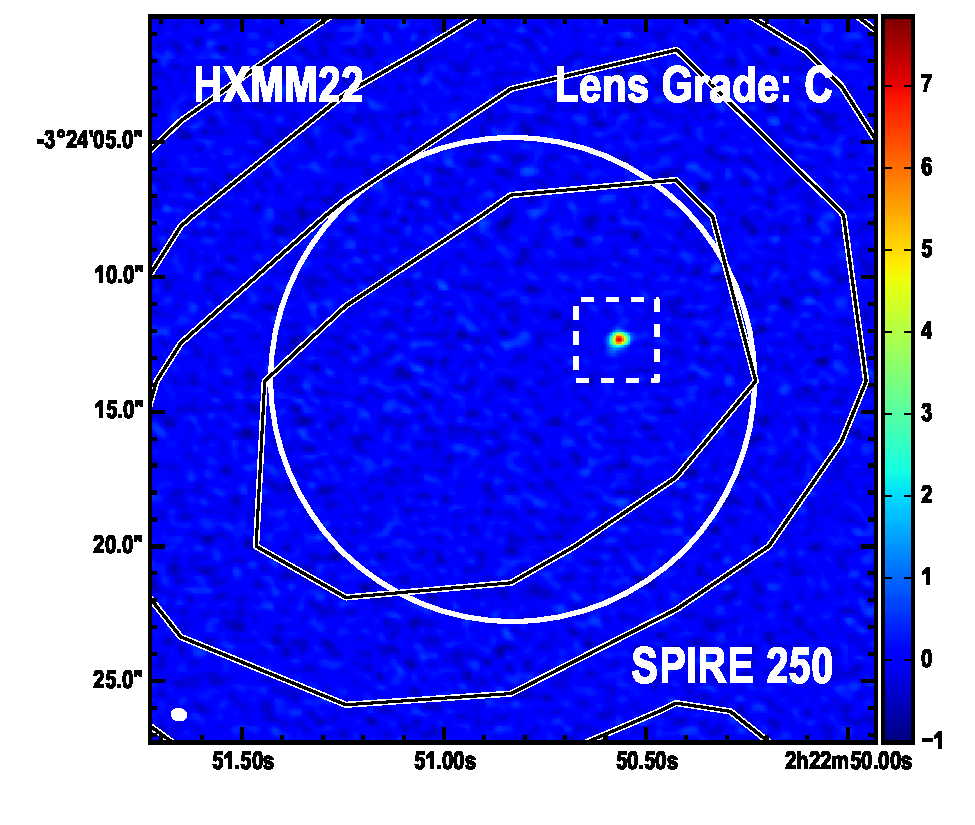
\includegraphics[width=0.331\textwidth]{../Figures/overlays/HXMM22_870_250.pdf}
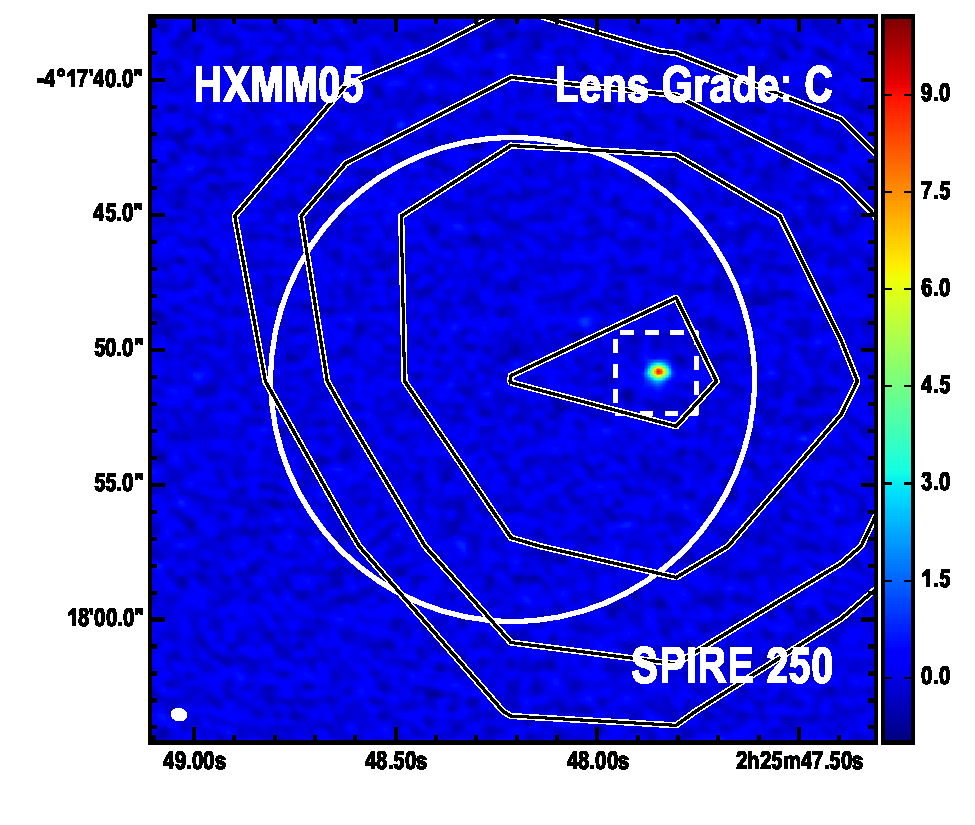
\includegraphics[width=0.331\textwidth]{../Figures/overlays/HXMM05_870_250.pdf}
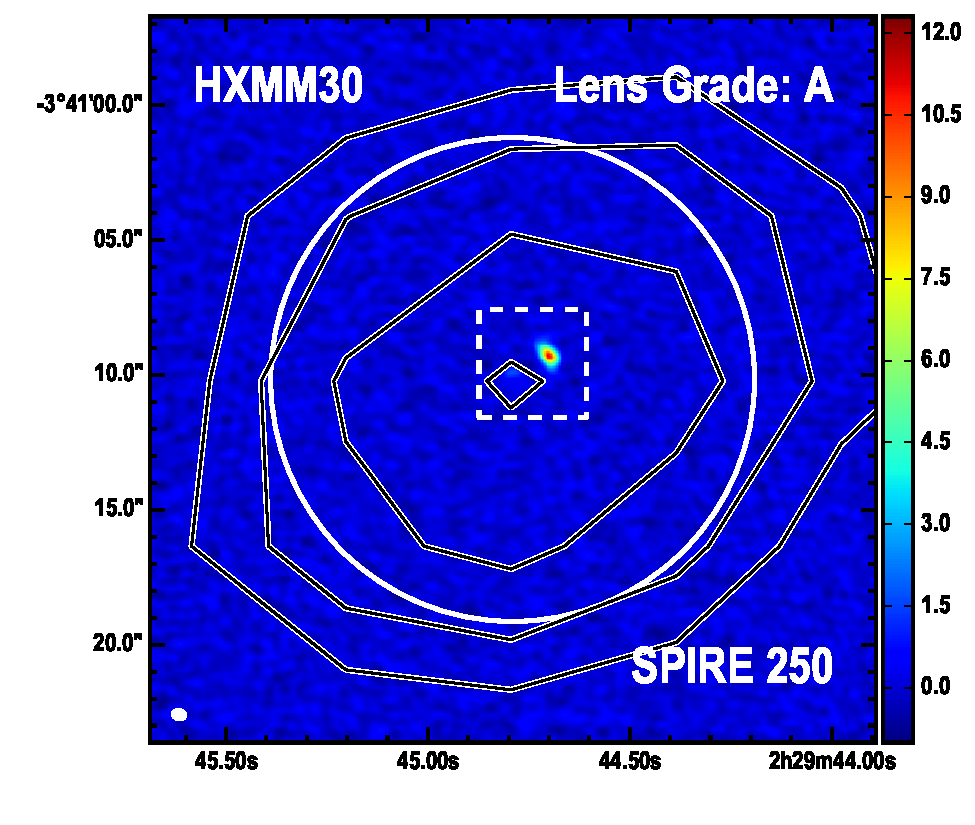
\includegraphics[width=0.331\textwidth]{../Figures/overlays/HXMM30_870_250.pdf}
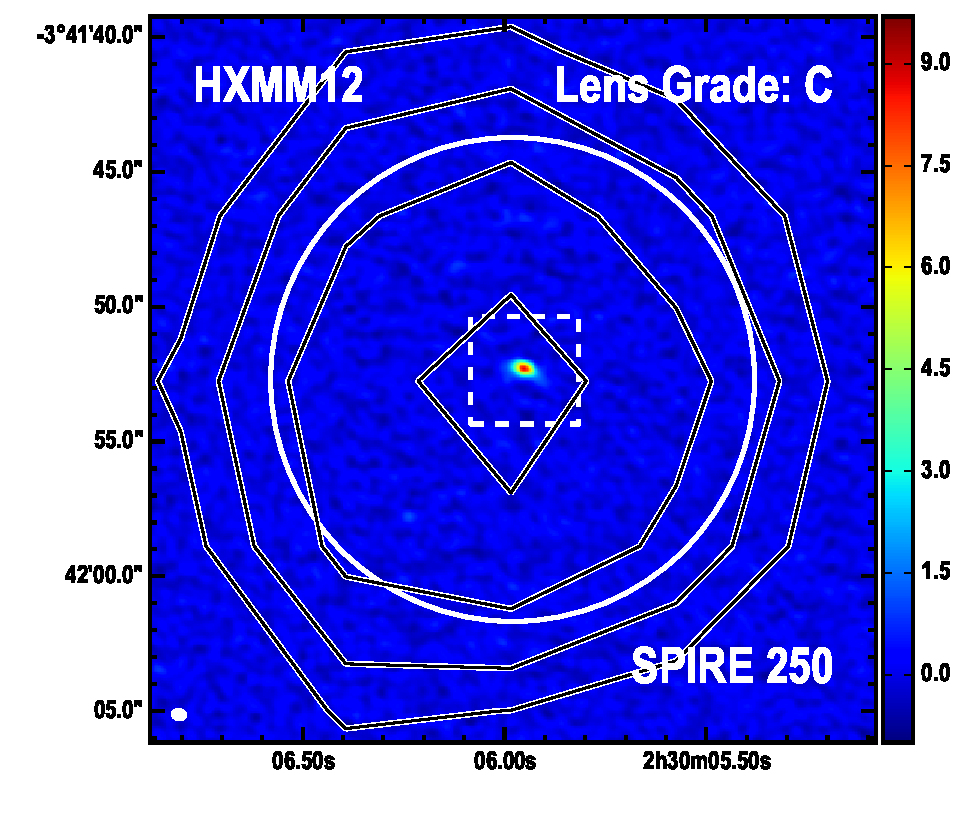
\includegraphics[width=0.331\textwidth]{../Figures/overlays/HXMM12_870_250.pdf}
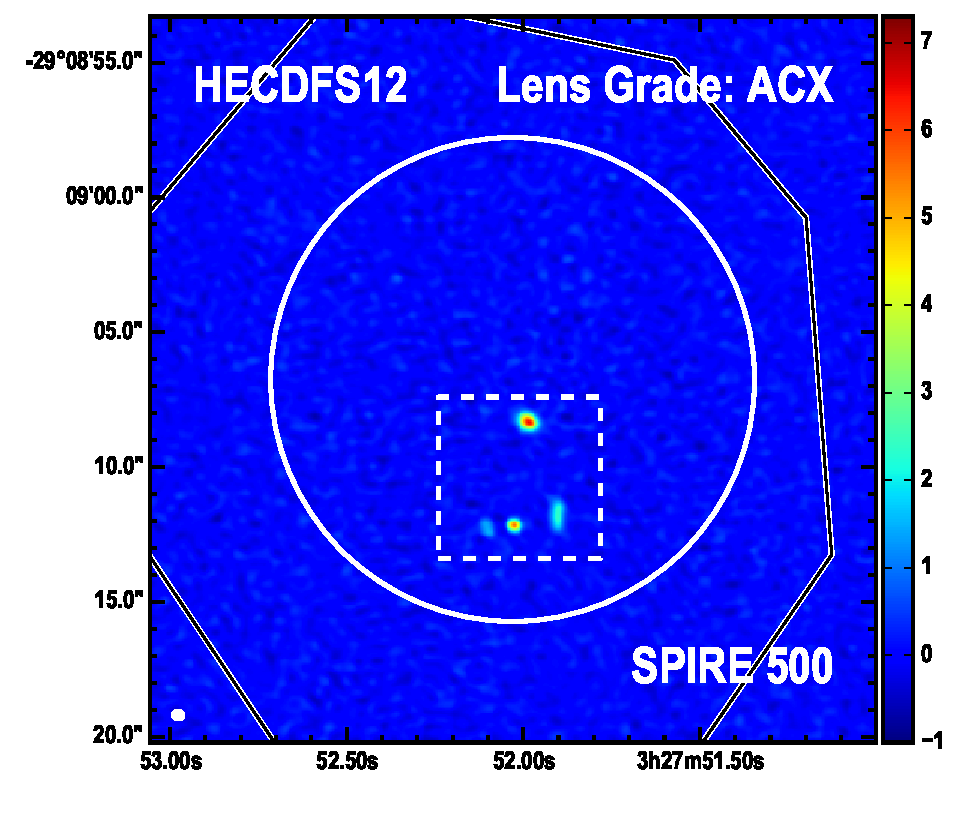
\includegraphics[width=0.331\textwidth]{../Figures/overlays/HECDFS12_870_500.pdf}
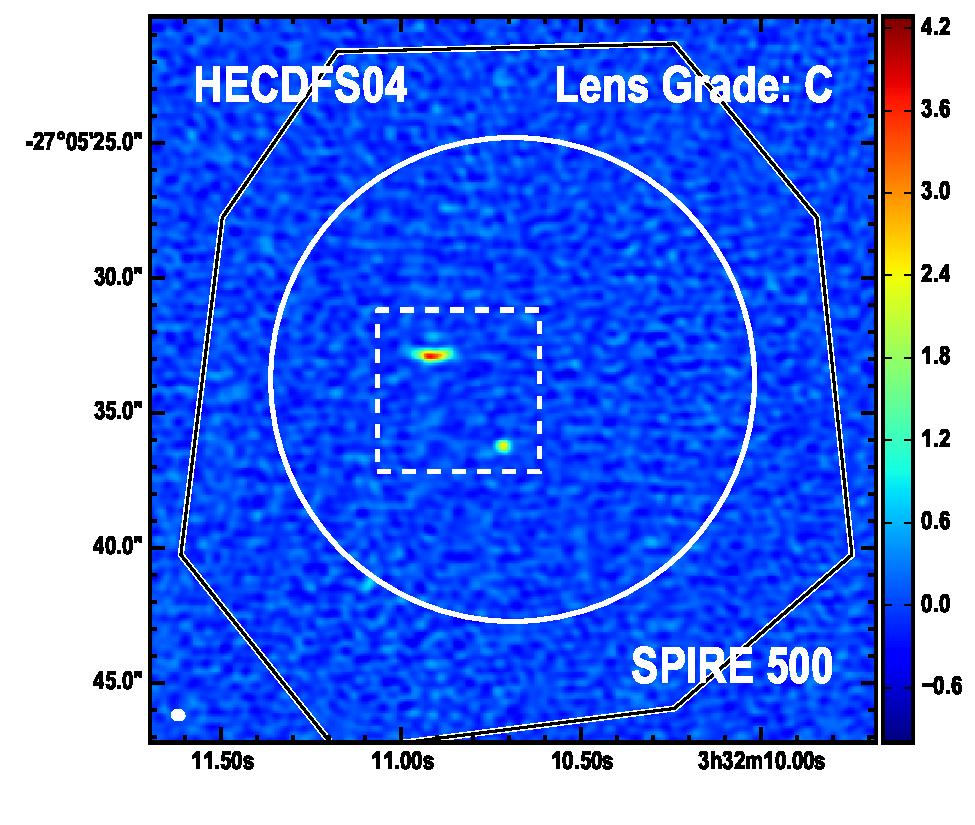
\includegraphics[width=0.331\textwidth]{../Figures/overlays/HECDFS04_870_500.pdf}
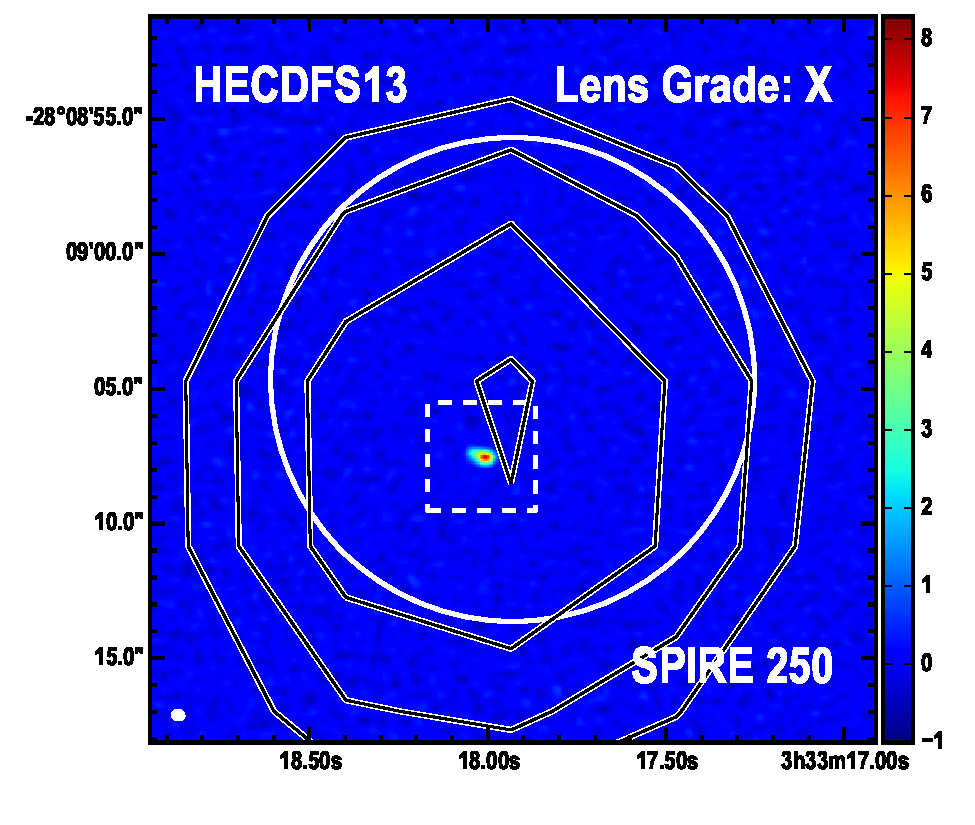
\includegraphics[width=0.331\textwidth]{../Figures/overlays/HECDFS13_870_250.pdf}
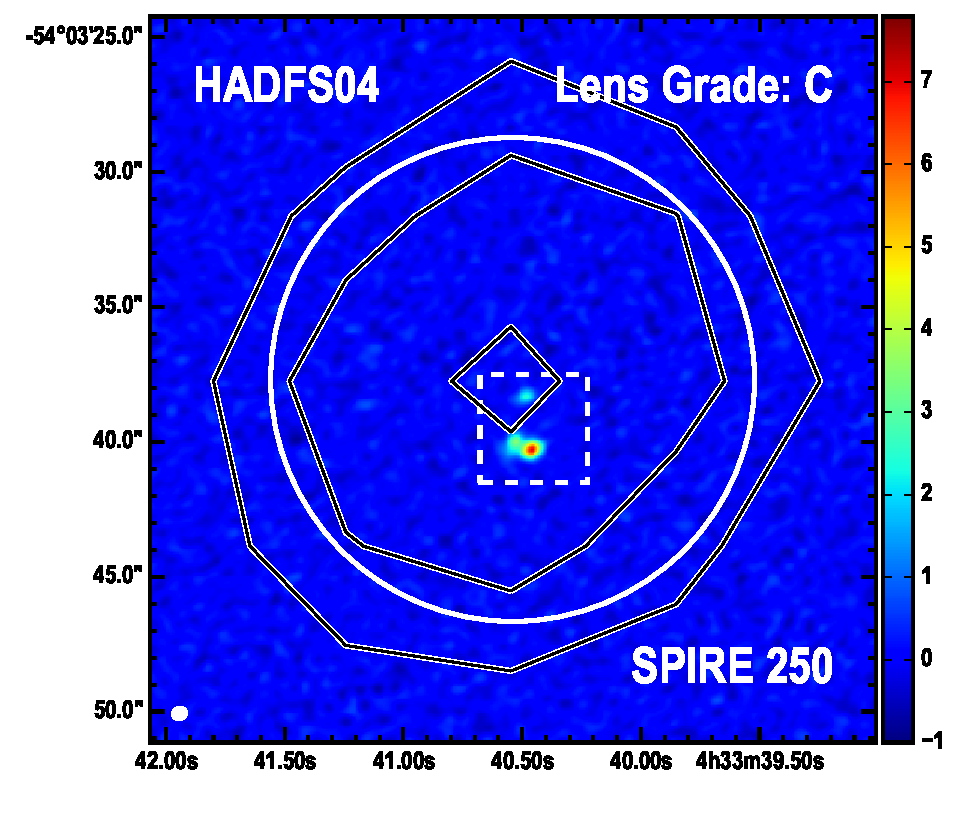
\includegraphics[width=0.331\textwidth]{../Figures/overlays/HADFS04_870_250.pdf}
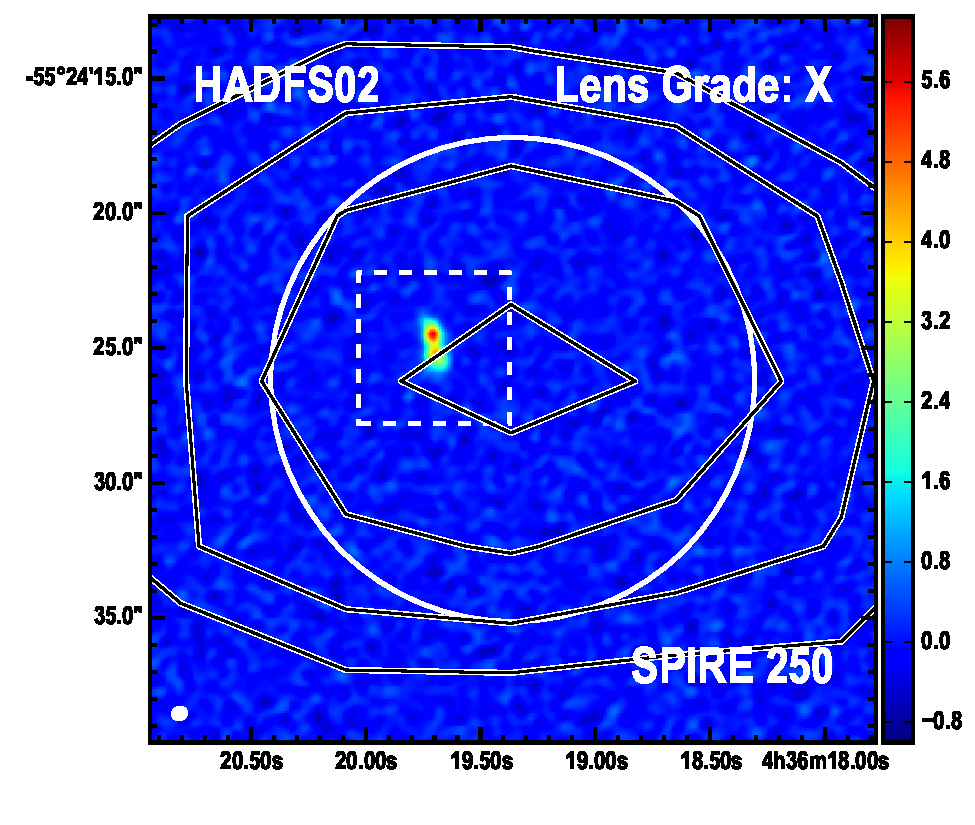
\includegraphics[width=0.331\textwidth]{../Figures/overlays/HADFS02_870_250.pdf}
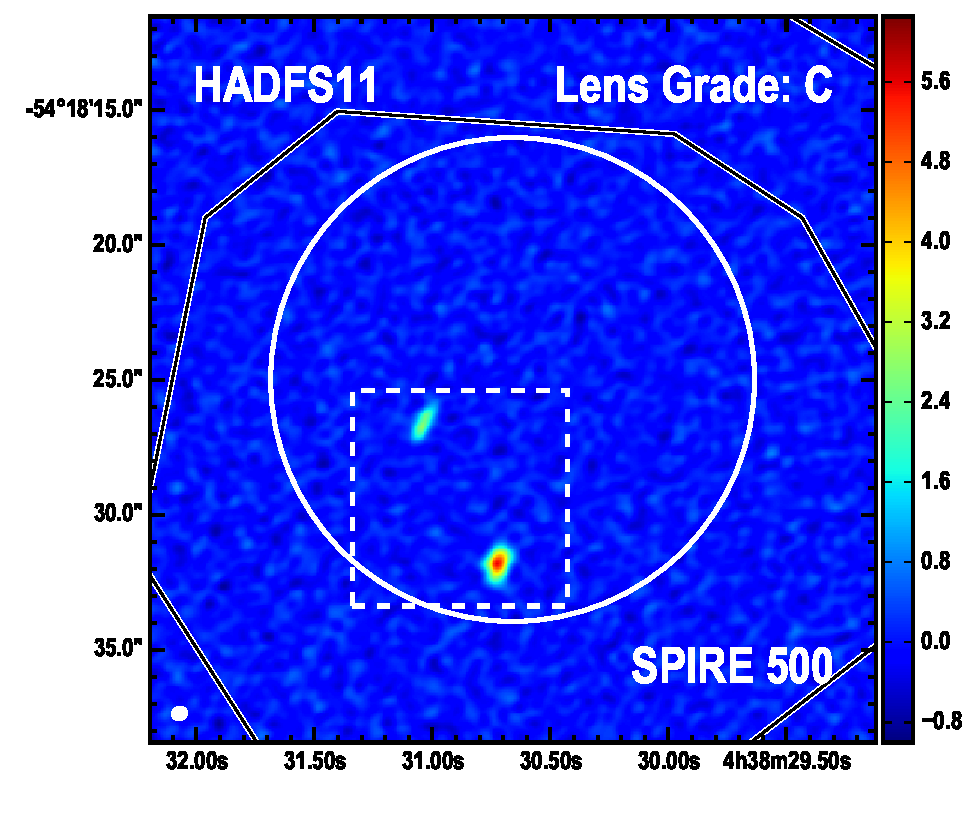
\includegraphics[width=0.331\textwidth]{../Figures/overlays/HADFS11_870_500.pdf}
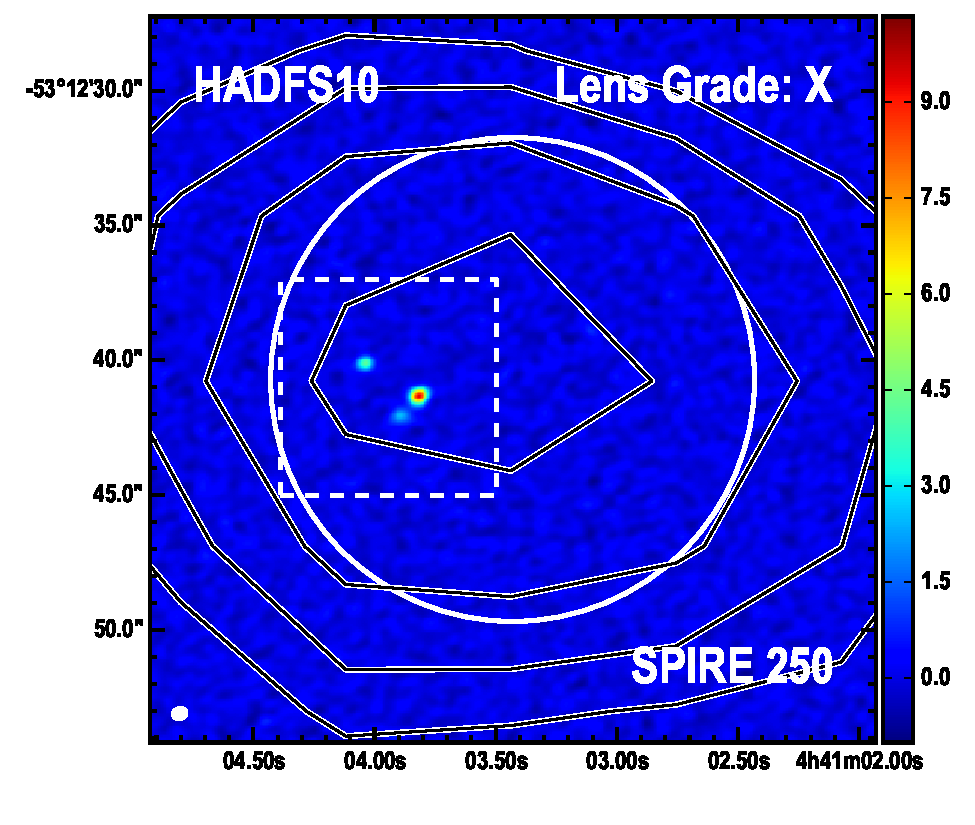
\includegraphics[width=0.331\textwidth]{../Figures/overlays/HADFS10_870_250.pdf}
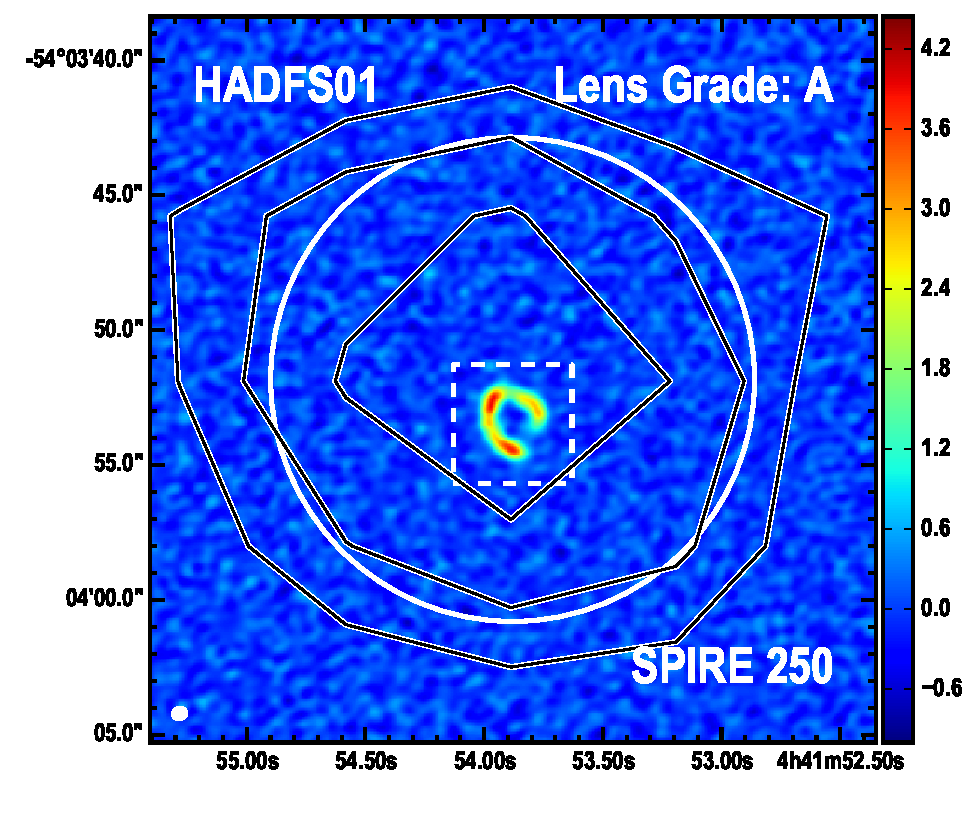
\includegraphics[width=0.331\textwidth]{../Figures/overlays/HADFS01_870_250.pdf}
\end{centering}

\caption{ Continued.}
\addtocounter{figure}{-1}

\end{figure*}

\begin{figure*}[!tbp] 
    \begin{centering}
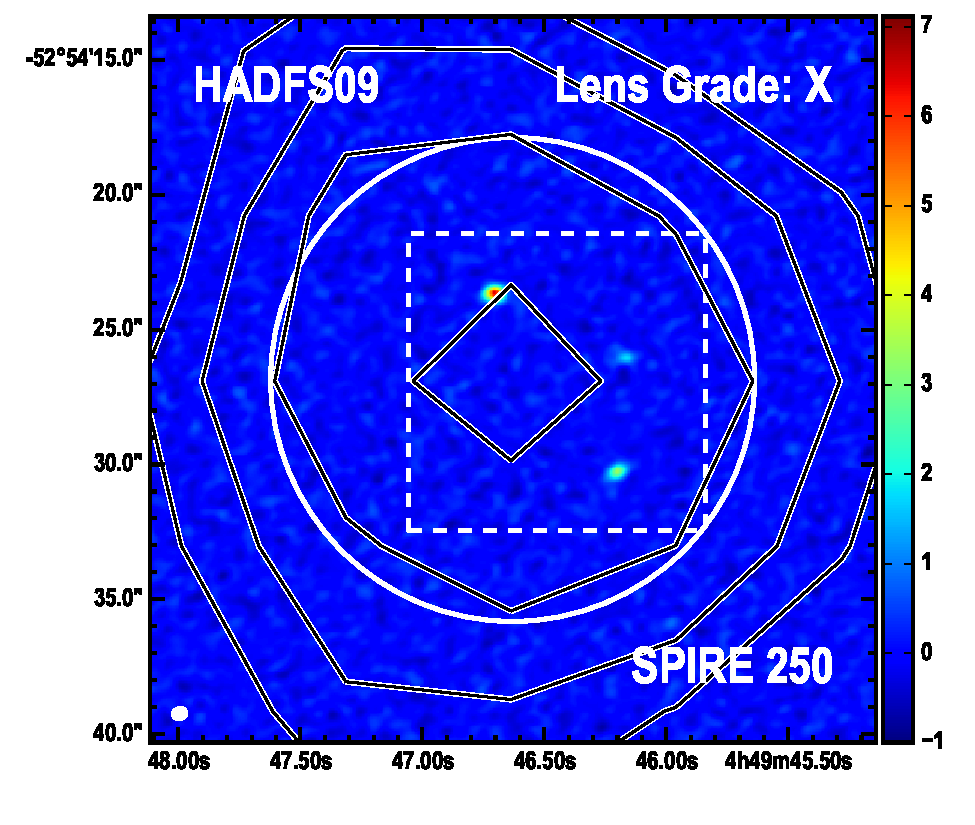
\includegraphics[width=0.331\textwidth]{../Figures/overlays/HADFS09_870_250.pdf}
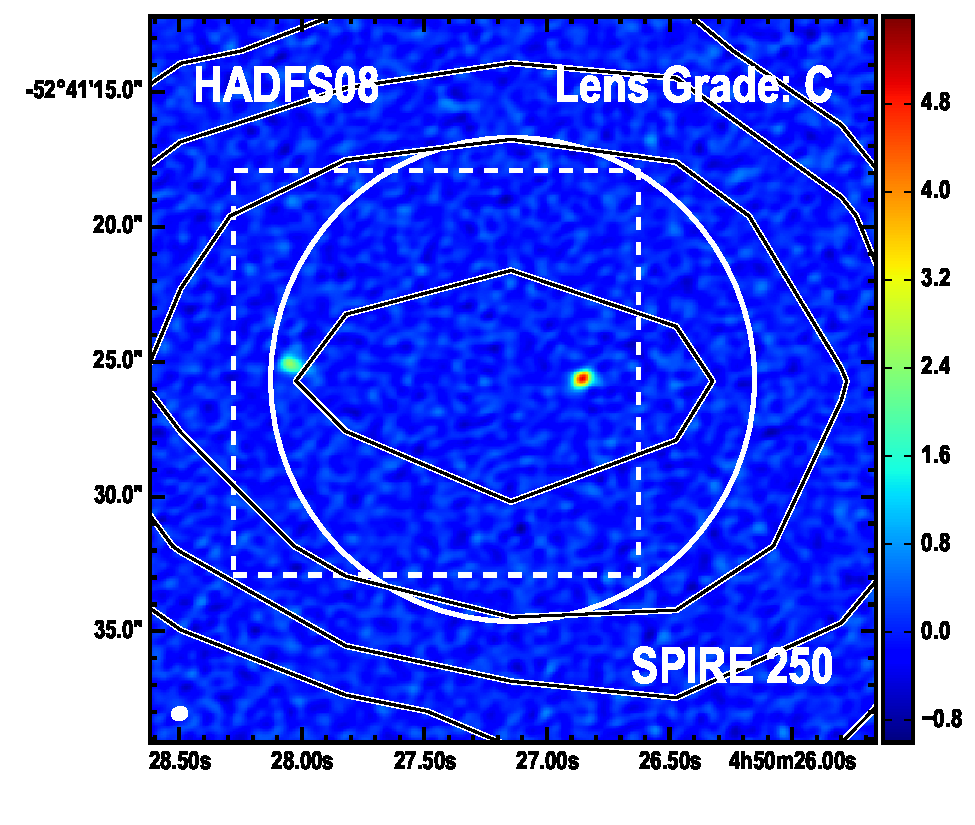
\includegraphics[width=0.331\textwidth]{../Figures/overlays/HADFS08_870_250.pdf}
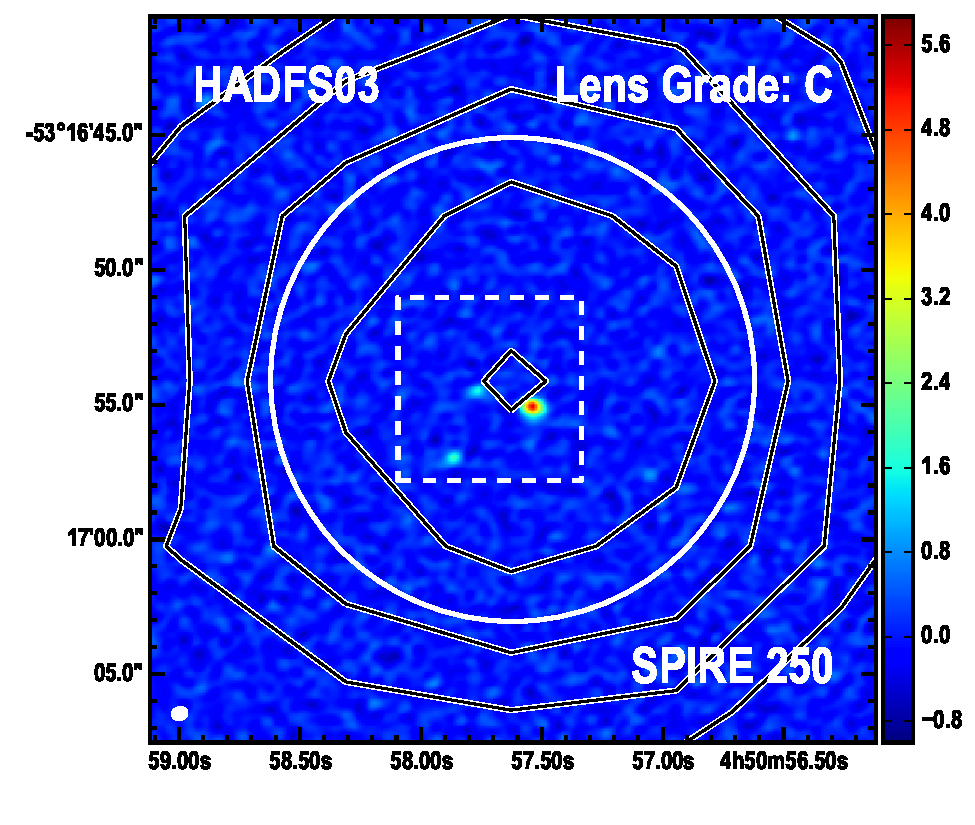
\includegraphics[width=0.331\textwidth]{../Figures/overlays/HADFS03_870_250.pdf}
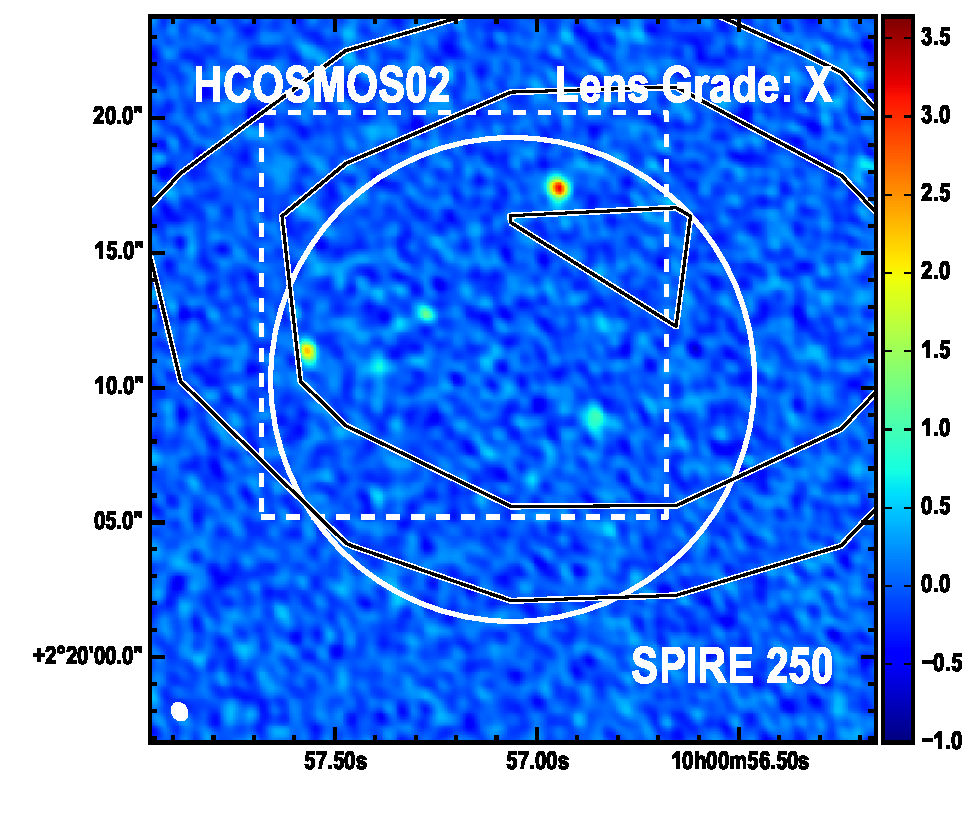
\includegraphics[width=0.331\textwidth]{../Figures/overlays/HCOSMOS02_870_250.pdf}
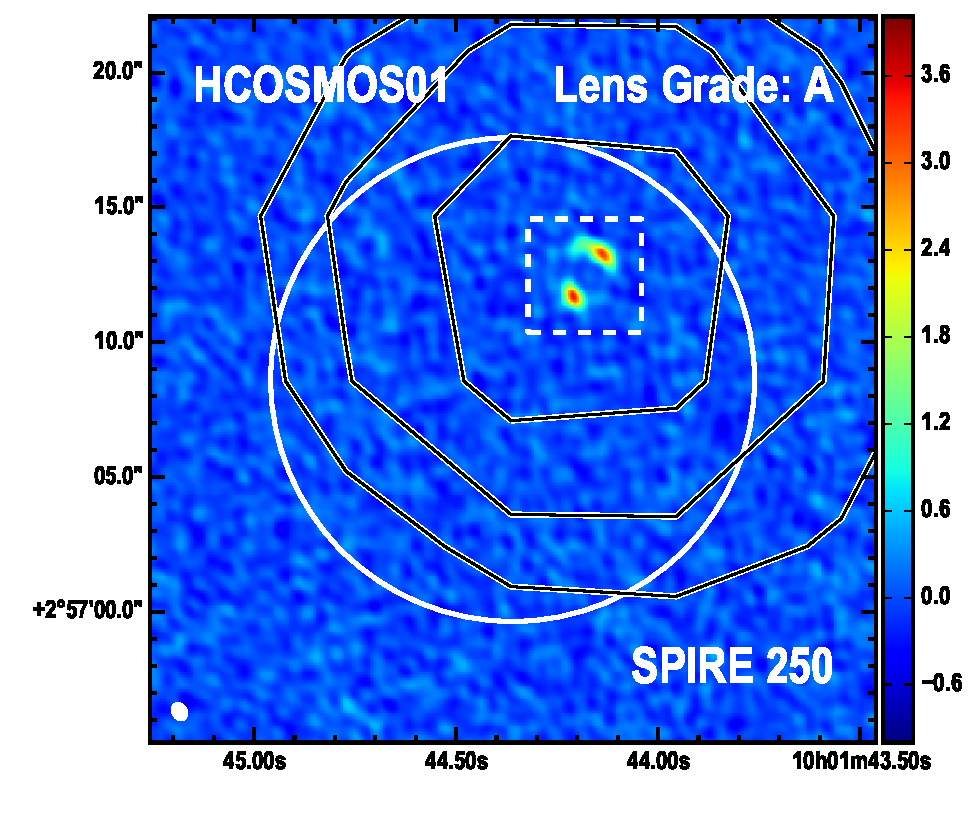
\includegraphics[width=0.331\textwidth]{../Figures/overlays/HCOSMOS01_870_250.pdf}
%\epsscale{1.00} 
%\includegraphics[width=\textwidth]{cutouts_dec17.png}
\end{centering}

\caption{ Continued.}
%\addtocounter{figure}{-1}

\end{figure*}

\section{Model Fits}\label{sec:modelfits}

\subsection{Model Fitting Methodology}\label{sec:modelfitsmeth}

An interferometer measures visibilities at discrete points in the {\it uv}
plane.  This is why pixel-to-pixel errors in the inverted and deconvolved
surface brightness map of an astronomical source are correlated.  The best way
to deal with this situation is to compare model and data visibilities rather
than surface brightness maps.  The methodology used in this paper is similar in
many aspects to that used in \citet{Bussmann:2012lr}, who presented the first
lens model derived from a visibility-plane analysis of interferometric imaging
of a strongly lensed DSFG discovered in wide-field submm surveys as well as
\citet{Bussmann:2013lr}, who extended this work to a statistically significant
sample of 30 objects.  It also bears some resemblence to the method used in
\citet{Hezaveh:2013fk}, who undertake lens modeling of interferometric data in
the visibility plane.  We summarize important information on the methodology
here, taking care to highlight where any differences occur between this work and
that of our previous efforts.

We created and made publicly available custom software, called {\sc uvmcmcfit},
that is capable of modeling all of the ALMA sources in this paper efficiently
and reliably.  

Sources are assumed to be elliptical Gaussians that are parameterized by the
following six free parameters: the position of the source (relative to the
primary lens if a lens is present) ($\Delta \alpha_{\rm s}$ and $\Delta
\delta_{\rm s}$), the total intrinsic flux density ($S_{\rm in}$), the
effective radius intermediate axis length ($r_{\rm s} = \sqrt{a_{\rm s} b_{\rm
s}}$), the axial ratio ($q_{\rm s}$ =  $b_{\rm s}/a_{\rm s}$), and the position
angle ($\phi_{\rm s}$, degrees east of north).  The use of an elliptical
Gaussian represents a simplification from the S\'ersic profile
\citep{1968adga.book.....S}  that is permitted based on the relatively weak
constraints on the S\'ersic index found in our previous work
\citep{Bussmann:2012lr, Bussmann:2013lr}.

When an intervening galaxy (or group of galaxies) is present along the line of
sight, {\sc uvmcmcfit} accounts for the deflection of light caused by this
structure using a simple ray-tracing routine that is adopted from a Python
routine written by A.~Bolton
\footnote{http://www.physics.utah.edu/$\sim$bolton/python\_lens\_demo/}.  This
represents a significant difference from \citet{Bussmann:2012lr} and
\citet{Bussmann:2013lr}, where we used the publicly available {\sc Gravlens}
software \citep{Keeton:2001lr} to map emission from the source plane to the
image plane for a given lensing mass distribution.  {\sc Gravlens} has a wide
range of lens mass profiles as well as a sophisticated algorithm for mapping
source-plane emission to the image-plane, but it also comes with a significant
input/output penalty that makes parallel computing prohibitively expensive.
For example, modeling a simple system comprising one lens and one source
typically required 24-48$\,$hours using the old software, whereas the same
system can be modeled in less than one hour with the pure-Python code.  The use
of pure-Python code for tracing the deflection of light rays is a critical
component of making {\sc uvmcmcfit} computationally feasible.

In {\sc uvmcmcfit}, lens mass profiles are represented by $N_{\rm lens}$
singular isothermal ellipsoid (SIE) profiles, where $N_{\rm lens}$ is the
number of lensing galaxies found from the best available optical or near-IR
imaging \citep[a multitude of evidence supports the SIE as a reasonable choice;
for a recent review, see][]{Treu:2010fk}.  Each SIE is fully described by the
following five free parameters: the position of the lens on the sky relative to
the arbitrarily chosen ``image center'' based on the ALMA 870$\,\mu$m emission
and any lensing galaxies seen in the optical or near-IR ($\Delta \alpha_{\rm
lens}$ and $\Delta \delta_{\rm lens}$; these can be compared with the position
of the optical or near-IR counterpart relative to the ``image center'': $\Delta
\alpha_{\rm NIR}$ and $\Delta \delta_{\rm NIR}$), the mass of the lens
(parameterized in terms of the intermediate axis angular Einstein radius,
$\theta_{\rm E}$), the axial ratio of the lens ($q_{\rm lens} = b_{\rm lens} /
a_{\rm lens}$), and the position angle of the lens ($\phi_{\rm lens}$; degrees
east of north).  Unless otherwise stated, when optical or near-IR imaging
suggests the presence of additional lenses (see Figure~\ref{fig:uvmodels}), we
estimate centroids for each lens by-eye and fix the positions of the additional
lenses with respect to the primary lens.  Each additional lens thus has 3 free
parameters: $\theta_{\rm E}$, $q_{\rm lens}$, and $\phi_{\rm lens}$.  We assume
secondary, tertiary, etc., lenses are located at the same redshift as the
primary lens.  

The total number of free parameters for any given system is $N_{\rm free} = 5 +
3 \times (N_{\rm lens} - 1) + 6 * N_{\rm source}$, where $N_{\rm source}$ is
the number of S\'ersic profiles used.

We use uniform priors for all model parameters.  The prior on the position of
the lenses covers $\pm0\farcs6$ ($1\farcs0$) in both RA and Dec, a value that
reflects the 1-$\sigma$ absolute astrometric solution between the ALMA and
optical/near-IR images of $0\farcs2$ ($0\farcs4$) for SDSS-based (2MASS-based)
astrometric calibration.  In section~\ref{sec:objectbyobject}, we discuss the
level of agreement between the astrometry from the images and the astrometry
from the lens modeling on an object-by-object basis.  For $\theta_{\rm E}$, the
prior covers $0\farcs1 - 6\arcsec$.  The axial ratios of the lenses and sources
are restricted to be $q_{\rm lens} > 0.3$ and $q_{\rm s} > 0.2$. No prior is
placed on the position angle of the lens or source.  The intrinsic flux density
for any source is allowed to vary from 0.1$\,$mJy to the total flux density
observed by the ALMA (we ensure that the posterior PDF of the intrinsic flux
density shows no signs of preferring a value lower than 0.1$\,$mJy).  The source
position is allowed to vary over any reasonable range necessary to fit the data
(typically, this is $\pm 1-2\arcsec$).  The effective radius is allowed to vary
from $0\farcs01 - 1\farcs5$.

The surface brightness map generated as part of {\sc uvmcmcfit} is then
converted to a ``simulated visibility'' dataset ($V_{\rm model}$) in much the
same way as MIRIAD's {\sc uvmodel} routine.  Indeed, the code used in {\sc
uvmcmcfit} is a direct Python port of {\sc uvmodel} (the use of {\sc uvmodel}
itself is not possible for the same reason as {\sc Gravlens}: constant
input/output makes parallel computing prohibitively expensive).  {\sc
uvmcmcfit} computes the Fourier transform of the surface brightness map and
samples the resulting visibilities in a way that closely matches the sampling
of the actual observed ALMA visibility dataset ($V_{\rm ALMA}$).

The quality of fit for a given set of model parameters is determined from the
maximum likelihood estimate $MLE$ according to the following equation:

\begin{equation}
    MLE = \sum_{u, v} \frac{|V_{\rm ALMA} - V_{\rm
    model}|^2}{\sigma^2} + log(2 \pi \sigma^2) 
\end{equation}

%\begin{equation}
%    MLE = -\frac{1}{2} (MLE_{\rm real} + MLE_{\rm imag}),
%\end{equation}

%\begin{equation}
%    MLE_{\rm real} = \sum_{u, v} \frac{[Re(V_{\rm ALMA}) - Re(V_{\rm
%    model})]^2}{\sigma^2} + log(2 \pi \sigma^2), 
%\end{equation}

%\begin{equation}
%    MLE_{\rm imag} = \sum_{u, v} \frac{[Im(V_{\rm ALMA}) - Im(V_{\rm
%    model})]^2}{\sigma^2} + log(2 \pi \sigma^2),
%\end{equation}

\noindent where $\sigma$ is the 1$\sigma$ uncertainty level for each
visibility and is determined from the scatter in the visibilities within a
single spectral window (this is a natural weighting scheme).  

We use {\sc emcee} \citep{Foreman-Mackey:2013yq} to sample the posterior
probability density function (PDF) of our model parameters.  {\sc emcee} is a
Markov chain Monte Carlo (MCMC) code that uses an affine-invariant ensemble
sampler to obtain significant performance advantages over standard MCMC
sampling methods \citep{goodmanweare}.  

We employ a ``burn-in'' phase with 512 walkers and 500-1000 iterations (i.e.,
$\approx 250,000-500,000$ samplings of the posterior PDF) to identify the
best-fit model parameters.  This position then serves as the basis to
initialize the ``final'' phase with 512 walkers and 10 iterations (i.e., 5,120
samplings of the posterior PDF) to determine uncertainties on the best-fit
model parameters.  
%The autocorrelation time for each parameter in a given ensemble of walkers and
%is of order unity for each parameter, implying that we have 5,000 independent
%samplings of the posterior PDF, more than enough to obtain a robust
%measurement of the mean and uncertainty on each parameter of the model.

During each MCMC iteration, we also measure the magnification factor at
870$\,\mu$m, $\mu_{870}$, for each source.  This is done simply by taking the
ratio of the total flux density in the lensed image of the model ($S_{\rm out}$
to the total flux density in the unlensed, intrinsic source model ($S_{\rm
in}$).  The use of an aperture when computing $\mu_{870}$ is important when
source profiles are used with significant flux at large radii (e.g., some types
of S\'ersic profiles).  For an elliptical Gaussian, such a step is unneccessary
(note that we did test this and found only $\approx 10\%$ difference between
$\mu_{870}$ computed with and without an aperture.  The best-fit value and
1$\sigma$ uncertainty on $\mu_{870}$ are drawn from the posterior PDF, as with
the other parameters of the model.

\subsection{Individual Model Fits}\label{sec:objectbyobject}

In this section, we present our model fits (as shown in
Figure~\ref{fig:uvmodels}) and describe each source in detail.

{\bf HELAISS02:} Four sources are detected by ALMA, all of which are weakly
lensed by a foreground galaxy seen in the {\it HST} image.  We assume an
Einstein radius of $1\farcs5$ for the lens as larger values begin to predict
counter images that are not seen by ALMA.  The magnification factors reported
here should be regarded as upper limits since we do not have strong constraints
on the lower limit of the Einstein radius of the lens (e.g., the magnication
factor for the source that is directly south of the lens is reported here to
have $\mu_{870} = 1.68 \pm 0.06$, but values as small as 1.1-1.2 are likely
plausible as well).  The ALMA sources are all detected by IRAC and their mid-IR
colors are similar, suggesting they lie at the same redshift (see
Figure~\ref{fig:iraccolor}).

{\bf HXMM02:} One source is detected by ALMA, and it is strongly lensed by one
foreground galaxy seen in the {\it HST} image.  The lensed source is not
detected in the {\it HST} image.  This object also has high quality SMA imaging
and an accompanying lens model that produces consistent results with those
given here \citep{Bussmann:2013lr}.

{\bf HXMM31:} Two sources are detected by ALMA, neither of which are lensed.
The faint, diffuse emission seen in the CFHT $i$-band image is atypical of
lensing galaxies.  The nearest bright galaxy seen at $i$-band is located
$\approx 18\arcsec$ southeast of the ALMA sources.

{\bf HXMM29:} Two sources are detected by ALMA, none of which appear to be
lensed.  The brighter ALMA source is weakly detected in the CFHT $i$-band
image.  

{\bf HXMM07:} One source is detected by ALMA, and it is strongly lensed by one
foreground galaxy detected in the Gemini-S image.  There is a $\approx
0\farcs5$ offset in the position of the foreground galaxy between the lens
model and the Gemini-S image.  Given the absolute astrometric uncertainty of
$0\farcs2$ (based on SDSS), we do not consider this offset to be significant.
The presence of a handful of $\pm3\sigma$ peaks in the residual map is likely
an indication that our assumption of a single Gaussian to describe the source
morphology is an oversimplification.

{\bf HXMM20:} Five sources are detected by ALMA, none of which appear to be
lensed.  There are a few faint smudges seen in the {\it HST} image which are
likely to be the rest-frame optical counterparts to the ALMA sources.  The ALMA
sources are all arranged in a chain like shape, possibly suggestive of a larger
filamentary overdensity in which they might reside.  IRAC imaging provides
support for this hypothesis (see Figure~\ref{fig:iraccolor}), as all of the ALMA
sources are detected and have similar mid-IR colors (suggesting they lie at
similar redshift).

{\bf HXMM01:} Three sources are detected by ALMA, all of which are weakly lensed
by two foreground galaxies seen in the {\it HST} and Keck/NIRC-II imaging.  The
ALMA imaging is broadly consistent with SMA data originally presented in
\citet{Fu:2013lr}, with two bright sources and a much fainter third source very
close to the more southern bright source.  We assume Einstein radii of
$0\farcs5$ for both lenses to reproduce the approach used in \citet{Fu:2013lr}.
This results in magnification factors for the three sources of $\mu_{870}
\approx 1.6 - 1.7$, similar to \citet{Fu:2013lr}.

{\bf HXMM04:} One source is detected by ALMA, and it is weakly lensed by a
foreground galaxy seen in the {\it HST} image.  We assume an Einstein radius of
$0\farcs5$ to represent the ``maximal lensing'' scenario.  Due to the
elliptical nature of the lens, this results in a magnification factor of
$\mu_{870} = 3.72 \pm 0.42$.  The {\it HST} morphology is complex: diffuse
emission to the north of the lens could be a detection of the background source
or could be a long spiral arm associated with the lensing galaxy.

{\bf HXMM09:} Two sources are detected by ALMA, both of which are weakly
lensed by a foreground galaxy detected in the {\it HST} image.  An Einstein
radius of $1\farcs5$ is used to represent the ``maximal lensing'' scenario and
results in magnification factors of $\mu_{870} = 2.25 \pm 0.17$ and $\mu_{870}
= 1.48 \pm 0.09$.

{\bf HXMM03:} Three sources are detected by ALMA, all of which are weakly lensed
by a foreground galaxy detected in the {\it HST} image and located $\approx
6\arcsec$ from the ALMA sources.  The central source is much brighter than the
other two sources, which makes fitting a model challenging.  We forced the
positions of the second and third sources to be at least $0\farcs5$ and
$-0\farcs5$ away from the first source in declination, respectively.
Furthermore, we fixed the position of the lens to be located $2\farcs5$ west
and $0\farcs5$ south of the image centroid given in Table~\ref{tab:position}.
We also fixed the Einstein radius to be $1\farcs0$, a typical value for
isolated galaxies in this sample and in \citet{Bussmann:2013lr}.  Because the
source is so far from the lens, the magnification factor is only $\mu_{870} =
1.19 \pm 0.01$.

{\bf HXMM11:} Two sources are detected by ALMA, both of which are weakly lensed.
This system is similar to HADFS08, although the two ALMA sources are much closer
and the lens must be less massive in order to avoid producing multiple images
of the closest ALMA source.  The fainter ALMA source has a much lower
magnification factor than the brighter source ($\mu_{870} = 1.10 \pm 0.01$ vs.
$\mu_{870} = 1.63 \pm 0.11$).  As with HADFS08, we caution that these
magnification factors represent the ``maximal lensing'' scenario and hence
should be considered upper limits.  Both ALMA sources are detected by IRAC and
have similar mid-IR colors, suggesting they lie at a similar redshift (see
Figure~\ref{fig:iraccolor}).

{\bf HXMM23:} One source is detected by ALMA, and it is coincident (within the
astrometric uncertainty) with a late-type galaxy seen in the {\it HST} image.
Here, we assume that the {\it HST} source is the true counterpart to the ALMA
source, implying that no lensing is occuring.  Consistent with this hypothesis
is that the SPIRE photometry show blue colors that suggest this object is at low
redshift.

{\bf HXMM22:} One source is detected by ALMA, and it appears to be unlensed.  A
faint smudge seen in the {\it HST} image of this source is due to a star
located $3\farcs5$ northeast of the ALMA source.

{\bf HXMM05:} One source is detected by ALMA, and it is weakly lensed by two
foreground galaxies seen in the {\it HST} images.  We assume an Einstein radius
of 1$\arcsec$ for the foreground lenses and fix the positions of both lenses
according to the location of the foreground galaxies in the {\it HST} image.
As with HXMM11, this is the ``maximal lensing'' scenario, so our magnification
measurement of $\mu_{870} = 1.80 \pm 0.16$ should be considered an upper limit.

{\bf HXMM30:} One source is detected by ALMA, and it is strongly lensed by one
foreground galaxy detected in the Gemini-S image.  As with HXMM07, there is a
$\approx 0\farcs5$ offset between the lens position according to the lens model
and the Gemini-S image.  We do not consider this offset significant.  An
alternative model in which the lens is sub-mm luminous cannot be ruled out, but
we consider this unlikely for a number of reasons.  First, it is a more complex
model (having two sources and one lens, rather than one source and one lens).
Second, lenses are very rarely detected in sub-mm imaging.  Third, the shape
and location of the ALMA sources relative to the Gemini-S source are typical of
strongly lensed objects (consistent with the very low residuals).  Fourth, the
alternative lens model predicts the lensed source to have an intrinsic flux
density of $\approx 13 \,$mJy, which would make it the brightest source in the
sample.

{\bf HXMM12:} One source is detected by ALMA, and it is weakly lensed by a group
of foreground galaxies seen in the {\it HST} image.  We assume an Einstein
radius of $0\farcs2$ for the nearest lensing galaxy and allow a $\pm0\farcs4$
shift in its position relative to that indicated by the {\it HST} image (which
has its astrometry tied to SDSS).  We represent the remaining members of the
group as a single SIS located $4\farcs5$ south and $4\farcs5$ east of the image
centroid and having an Einstein radius of $2\farcs0$.  This is meant to
represent the ``maximal lensing'' scenario, so our measurement of $\mu_{870}$
should be regarded as an upper limit.  The presence of two $3\sigma$ peaks
located near the center of the residual image indicates that the model does not
fit the data perfectly.  This could be an indication that either of our
assumptions for the lens potential or source structure are oversimplifications.
Higher resolution imaging is needed to determine the most likely cause.

{\bf HECDFS12:} This is a complex, very well constrained system.  Two sources
are detected by ALMA: one is strongly lensed and the other is weakly lensed.
In addition, the lens is detected by ALMA (this is one of two sources in the
entire ALMA sample that is unresolved by ALMA).  These facts work together to
provide very tight constraints on the system.  Since the lens is detected by
ALMA, its position relative to the lensed images is unambiguous.  Also, because
there is a strongly lensed source with multiple images, the Einstein radius of
the lens is unambiguous.  A byproduct of these two facts is that the
magnification factor of the weakly lensed source is known to very high
precision as well.  It experiences a magnification factor of $\mu_{870} =
1.520\pm0.002$ despite being located $\approx4\arcsec$ north of the lens (which
has an Einstein radius of $1.353\pm0.005$).  We use these numbers to inform our
estimates of the Einstein radius for weakly lensed sources without the
excellent contraints provided by this system.  Finally, this source is detected
(and unresolved) in the NRAO VLA Sky Survey \citep{Condon:1998uq}, having
$S_{\rm 1.4\,GHz} = 21.8 \pm 0.8\,$mJy.  Assuming all of this radio emission
originates from the lens, this implies a spectral slope of $\alpha = -0.24$ and
is consistent with non-thermal emission from the lens.

{\bf HECDFS04:} Two sources are detected by ALMA, both of which are weakly
lensed by a foreground galaxy seen in the {\it HST} image.  There is also a
3$\sigma$ peak coincident with {\it HST} source that may be an indication that
the lens has been detected by ALMA.  We do not attempt to model this 3$\sigma$
peak.  We assume an Einstein radius of $0\farcs5$ for the lens, since larger
values predict the existence of counter images that are not seen by ALMA.  The
second ALMA source is located $\approx5\arcsec$ from the lens and experiences a
small but significant magnification of $\mu_{870} = 1.12 \pm 0.02$.  Both ALMA
sources appear to be detected by IRAC and have similar mid-IR colors, suggesting
they lie at the same redshift (see Figure~\ref{fig:iraccolor}).  

{\bf HECDFS13:} This system is very similar to HADFS02, except that here the two
ALMA sources are separated by $\approx 0\farcs4$ rather than $0\farcs8$ and one
source is brighter than the other by a factor of 2.  Assuming the two sources
have similar mass to light ratios, their brightness ratios indicate major
merger rather than minor merger activity.  The projected physical distance is
$\approx 2-3$kpc, assuming a redshift of $z=2$ for the ALMA sources.  This
could be an example of a major merger approaching final coalescence and
experiencing a significant boost in star-formation due to enhancements in the
local gas density brought about by tidal forces during the merger.

{\bf HADFS04:} Three sources are detected by ALMA, all of which are weakly
lensed by a foreground galaxy seen in the {\it HST} image.  We assume an
Einstein radius of $0\farcs5$ for the lens, as values larger than this produce
multiple images of the ALMA sources.  Based on the brightness of the lens, we
consider to be unlikely values for the Einstein radius that are smaller than
$0\farcs5$, so the results we report for this object should be robust.

{\bf HADFS02:} Two sources are detected by ALMA.  The nearest possible lens is
located $\approx 8\arcsec$ from the ALMA sources, indicating that lensing is
likely to be irrelevant in this system.  The two ALMA sources are similarly
bright ($S_{870} = 8.27 \pm 0.53\,$mJy and $S_{870} = 9.07 \pm 0.27\,$mJy) and
separated by $\approx 0\farcs8$, corresponding to a projected physical distance
of $\approx 6\,$kpc. This distance is typical of the pericentric passage
distance in both hydrodynamical simulations of major mergers
\citep[e.g.,][]{Hayward:2012lr} and CO observations of major mergers
\citep[e.g.,][]{2008ApJ...680..246T, 2010ApJ...724..233E, 2011ApJ...733L..11R,
2011MNRAS.412.1913I}.  Two plausible scenarios are that HADFS02 represents a
major merger that just experienced a first pass or is approaching final
coalescence, either of which significantly enhanced star-formation in the
system.

{\bf HADFS11:} Two sources are detected by ALMA, both of which are weakly
lensed by a group of small galaxies detected in the {\it HST} image.  We
represent the gravitational potential of the group with a single SIE lens and
an Einstein radius of $1\farcs0$.  Values larger than this produce additional
counter images that are not seen in the ALMA imaging.  We cannot rule out
smaller Einstein radii, but we consider these unlikely given the number of
sources and their brightness in the {\it HST} image.

{\bf HADFS10:} Three sources are detected by ALMA.  In this paper, we have
assumed that all three are unlensed.  There is a group of three sources
detected in our Gemini-S optical imaging located $\approx 7\arcsec$ east of the
ALMA sources.  This distance is so large that plausible mass ranges for the
Gemini-S sources would imply at most a factor of 1.1-1.2 boost in the apparent
flux densities of the ALMA sources.

{\bf HADFS01:} This is a single source that is strongly lensed by a foreground
galaxy seen in the {\it HST} image.  The lensed source is not detected by {\it
HST}.  The source is highly elongated ($q_s = 0.31 \pm 0.01$), but fits the
data very well.  The position of the lens according to the lens model is
consistent with the position in the {\it HST} image given the $0\farcs4$
fundamental uncertainty due to using the 2MASS system as the fundamental basis
for the astrometry.

{\bf HADFS09:} Three sources are detected by ALMA, none of which appear to be
lensed (the closest bright {\it HST} source is located $\approx 13\arcsec$ away
from the ALMA sources).

{\bf HADFS08:} Two sources are detected by ALMA, both of which are weakly lensed
by a foreground galaxy in the {\it HST} image.  The ALMA sources have the
largest separation of any in our sample overall: $\approx 10\arcsec$.  We
assume an Einstein radius of $1\farcs5$ for the foreground lens as a ``maximal
lensing'' scenario.  This results in magnification factors of $\mu_{870} = 2.3
\pm 0.1$ and $\mu_{870} = 1.2 \pm 0.1$ for the two sources.  Our constraints on
the true Einstein radius of the lens are weak, so these values for $\mu_{870}$
should be regarded as upper limits.

{\bf HADFS03:} Three sources are detected by ALMA, each of which is weakly
lensed by a bright foreground galaxy seen in the {\it HST} image.  Alternative
scenarios involving strong lensing can be ruled out by the location of the
lens: $\approx 2-3\arcsec$ north of the centroid of the ALMA sources (the rms
error in the astrometry is set from 2MASS at a level of $\approx 0\farcs4$) as
well as the unusual location and fluxes of the ALMA sources relative to each
other.  We assume an Einstein radius of $0\farcs5$ and fix the position angle
of the lens to be between 40-50 degrees to match the orientation seen in the
{\it HST} image.  Larger Einstein radii can be ruled out by the absence of
counter images north of the lens.

{\bf HCOSMOS02:} Five sources are detected by ALMA \citep[the brightest of
which has already been detected;][]{Smolcic:2012zl}, none of which appear to be
lensed.  Previous research has shown this to be an overdense region \citep[this
object is called COSBO3 in][]{Aravena:2010fr} with a photometric redshift of
$z=2.3-2.4$.  Our ALMA imaging offers the first convincing evidence that the
associated galaxies in the overdensity are sub-mm bright and thus intensely
star-forming.  There are a number of $2-3\sigma$ peaks in the map that could be
real.  This would further increase the multiplicity rate for this object, but
we caution that there are also negative peaks of similar amplitude (i.e.,
$2-3\sigma$) present in this map.  Some of the ALMA sources have counterparts
detected in the {\it HST} image, whereas all of the ALMA sources are detected
by IRAC (see Figure~\ref{fig:iraccolor}).  Their mid-IR colors are similar,
providing further evidence that the ALMA sources lie at the same redshift.  

{\bf HCOSMOS01:} This system is similar to HADFS01: a single source that is
strongly lensed by a foreground galaxy seen in the {\it HST} image.  In fact,
the background source is also detected by {\it HST} as well as Keck/NIRC-II
adaptive optics imaging, and a lens model has been published based on these
data \citep{Calanog:2014lr}.  The morphology of the lensed emission is very
different between the Keck and ALMA imaging, suggesting differential
magnification is important in this object.  The very small sizes of the sources
are consistent with this as well ($r_s = 0.023 \pm 0.003\arcsec$, Keck and $r_s
= 0.055 \pm 0.007\arcsec$, ALMA).  Adopting a redshift of $z=2$ for the lensed
source implies physical sizes of $\approx 150\,$pc and $\approx 300\,$pc for
the rest-frame optical and rest-frame FIR, respectively.

\begin{figure*}[!tbp] 
    \begin{centering}
%\epsscale{1.00} 
%\includegraphics[width=\textwidth]{cutouts_dec17.png}
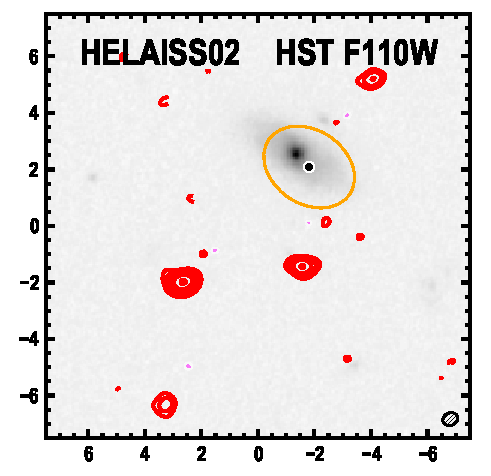
\includegraphics[width=0.162\textwidth]{../Figures/modelfit/HELAISS02_optical_bestfit.pdf}
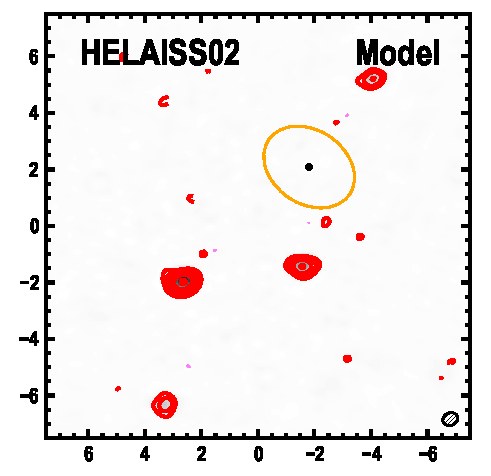
\includegraphics[width=0.162\textwidth]{../Figures/modelfit/HELAISS02_model_bestfit.pdf}
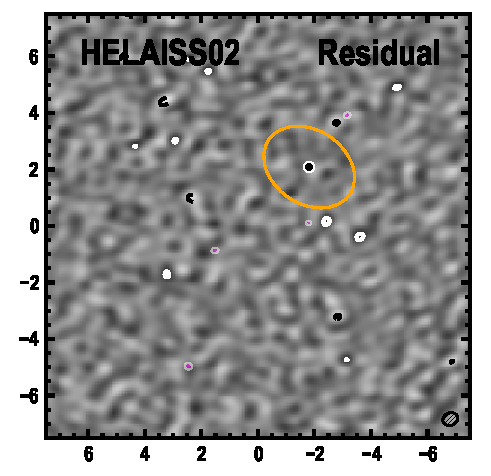
\includegraphics[width=0.162\textwidth]{../Figures/modelfit/HELAISS02_residual_bestfit.pdf}
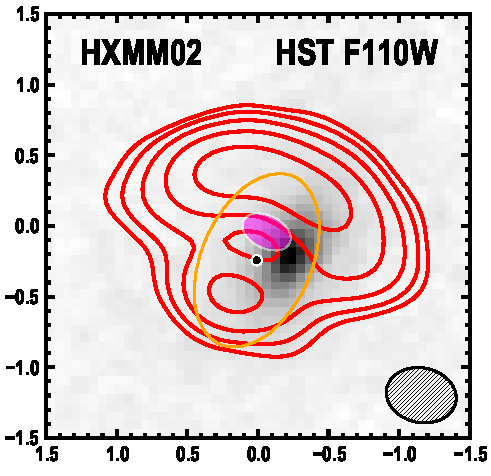
\includegraphics[width=0.162\textwidth]{../Figures/modelfit/HXMM02_optical_bestfit.pdf}
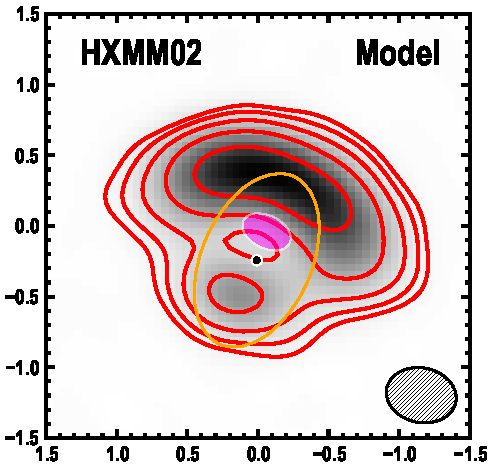
\includegraphics[width=0.162\textwidth]{../Figures/modelfit/HXMM02_model_bestfit.pdf}
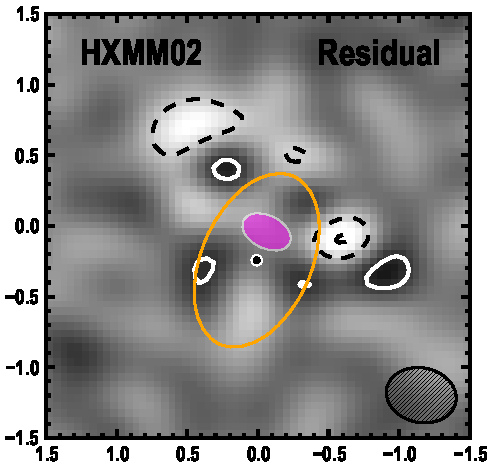
\includegraphics[width=0.162\textwidth]{../Figures/modelfit/HXMM02_residual_bestfit.pdf}
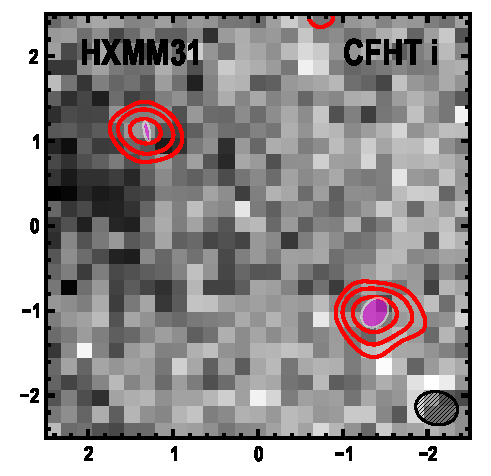
\includegraphics[width=0.162\textwidth]{../Figures/modelfit/HXMM31_optical_bestfit.pdf}
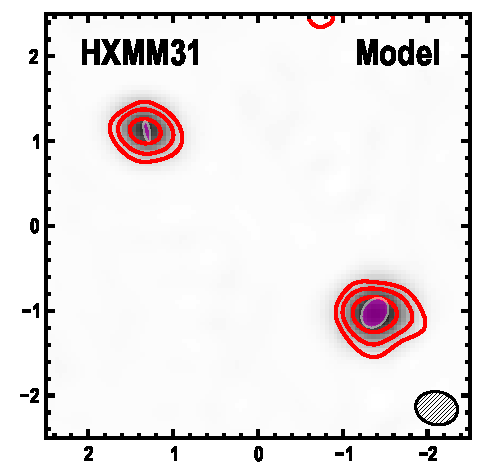
\includegraphics[width=0.162\textwidth]{../Figures/modelfit/HXMM31_model_bestfit.pdf}
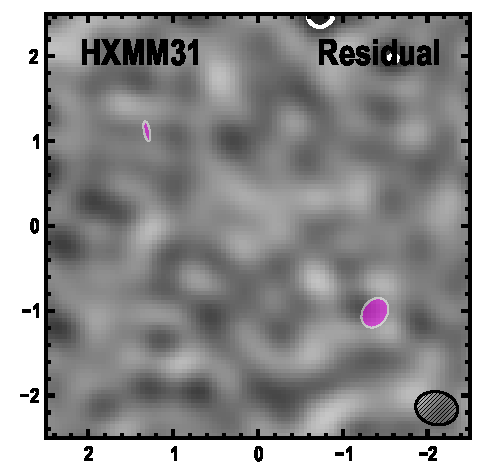
\includegraphics[width=0.162\textwidth]{../Figures/modelfit/HXMM31_residual_bestfit.pdf}
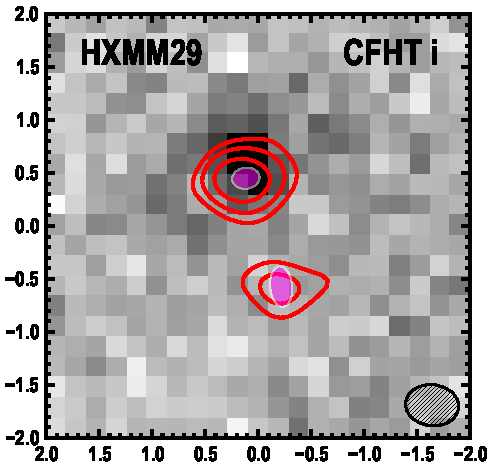
\includegraphics[width=0.162\textwidth]{../Figures/modelfit/HXMM29_optical_bestfit.pdf}
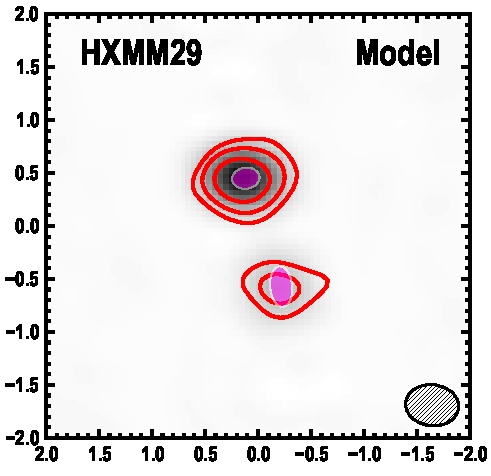
\includegraphics[width=0.162\textwidth]{../Figures/modelfit/HXMM29_model_bestfit.pdf}
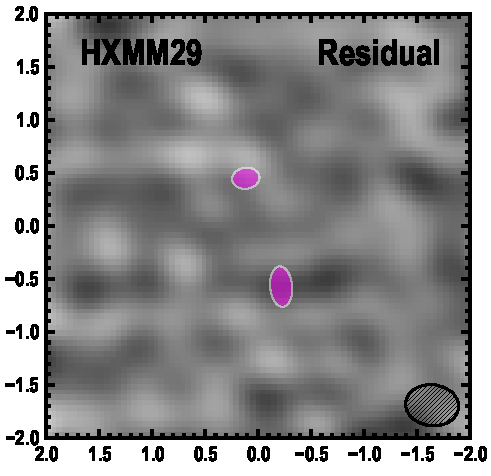
\includegraphics[width=0.162\textwidth]{../Figures/modelfit/HXMM29_residual_bestfit.pdf}
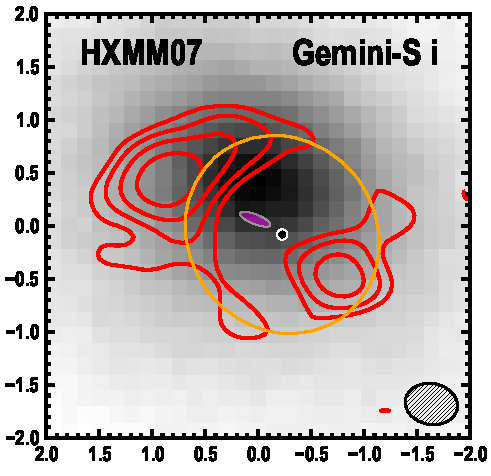
\includegraphics[width=0.162\textwidth]{../Figures/modelfit/HXMM07_optical_bestfit.pdf}
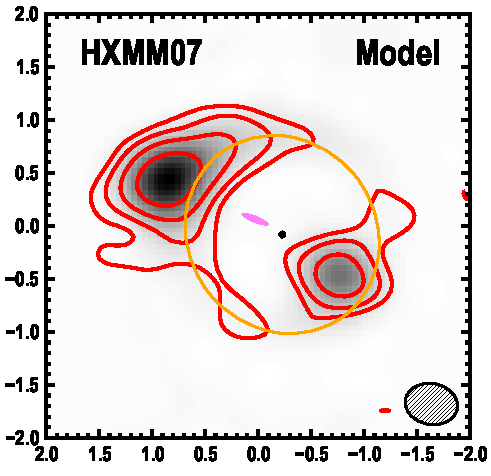
\includegraphics[width=0.162\textwidth]{../Figures/modelfit/HXMM07_model_bestfit.pdf}
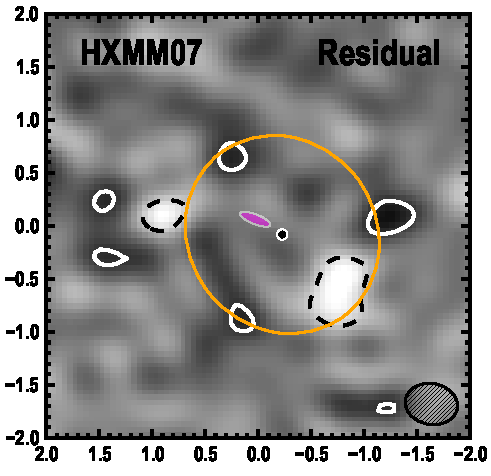
\includegraphics[width=0.162\textwidth]{../Figures/modelfit/HXMM07_residual_bestfit.pdf}
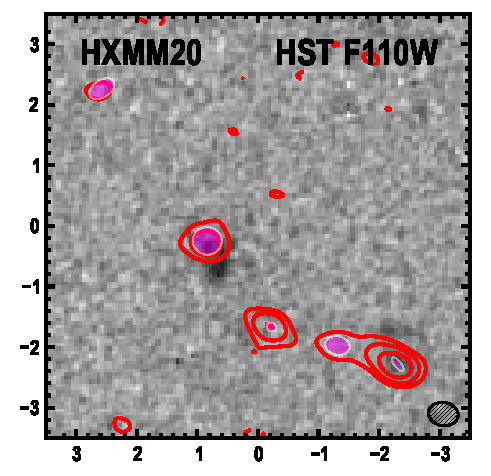
\includegraphics[width=0.162\textwidth]{../Figures/modelfit/HXMM20_optical_bestfit.pdf}
\includegraphics[width=0.162\textwidth]{../Figures/modelfit/HXMM20_model_bestfit.pdf}
\includegraphics[width=0.162\textwidth]{../Figures/modelfit/HXMM20_residual_bestfit.pdf}
\includegraphics[width=0.162\textwidth]{../Figures/modelfit/HXMM01_optical_bestfit.pdf}
\includegraphics[width=0.162\textwidth]{../Figures/modelfit/HXMM01_model_bestfit.pdf}
\includegraphics[width=0.162\textwidth]{../Figures/modelfit/HXMM01_residual_bestfit.pdf}
\includegraphics[width=0.162\textwidth]{../Figures/modelfit/HXMM04_optical_bestfit.pdf}
\includegraphics[width=0.162\textwidth]{../Figures/modelfit/HXMM04_model_bestfit.pdf}
\includegraphics[width=0.162\textwidth]{../Figures/modelfit/HXMM04_residual_bestfit.pdf}
\includegraphics[width=0.162\textwidth]{../Figures/modelfit/HXMM09_optical_bestfit.pdf}
\includegraphics[width=0.162\textwidth]{../Figures/modelfit/HXMM09_model_bestfit.pdf}
\includegraphics[width=0.162\textwidth]{../Figures/modelfit/HXMM09_residual_bestfit.pdf}
\includegraphics[width=0.162\textwidth]{../Figures/modelfit/HXMM03_optical_bestfit.pdf}
\includegraphics[width=0.162\textwidth]{../Figures/modelfit/HXMM03_model_bestfit.pdf}
\includegraphics[width=0.162\textwidth]{../Figures/modelfit/HXMM03_residual_bestfit.pdf}
\includegraphics[width=0.162\textwidth]{../Figures/modelfit/HXMM11_optical_bestfit.pdf}
\includegraphics[width=0.162\textwidth]{../Figures/modelfit/HXMM11_model_bestfit.pdf}
\includegraphics[width=0.162\textwidth]{../Figures/modelfit/HXMM11_residual_bestfit.pdf}
\includegraphics[width=0.162\textwidth]{../Figures/modelfit/HXMM23_optical_bestfit.pdf}
\includegraphics[width=0.162\textwidth]{../Figures/modelfit/HXMM23_model_bestfit.pdf}
\includegraphics[width=0.162\textwidth]{../Figures/modelfit/HXMM23_residual_bestfit.pdf}
\includegraphics[width=0.162\textwidth]{../Figures/modelfit/HXMM22_optical_bestfit.pdf}
\includegraphics[width=0.162\textwidth]{../Figures/modelfit/HXMM22_model_bestfit.pdf}
\includegraphics[width=0.162\textwidth]{../Figures/modelfit/HXMM22_residual_bestfit.pdf}
\includegraphics[width=0.162\textwidth]{../Figures/modelfit/HXMM05_optical_bestfit.pdf}
\includegraphics[width=0.162\textwidth]{../Figures/modelfit/HXMM05_model_bestfit.pdf}
\includegraphics[width=0.162\textwidth]{../Figures/modelfit/HXMM05_residual_bestfit.pdf}
\includegraphics[width=0.162\textwidth]{../Figures/modelfit/HXMM30_optical_bestfit.pdf}
\includegraphics[width=0.162\textwidth]{../Figures/modelfit/HXMM30_model_bestfit.pdf}
\includegraphics[width=0.162\textwidth]{../Figures/modelfit/HXMM30_residual_bestfit.pdf}
\includegraphics[width=0.162\textwidth]{../Figures/modelfit/HXMM12_optical_bestfit.pdf}
\includegraphics[width=0.162\textwidth]{../Figures/modelfit/HXMM12_model_bestfit.pdf}
\includegraphics[width=0.162\textwidth]{../Figures/modelfit/HXMM12_residual_bestfit.pdf}
\end{centering}

\caption{ Model fits for each target in the ALMA sample, 3 panels per target.
{\it Left}: ALMA 870$\mu$m imaging (red contours, starting at $\pm 3\sigma$ and
increasing by factors of 2) overlaid on best available optical or near-IR
imaging (grayscale, with telescope and filter printed in upper right corner).
The location and morphology of all sources used in the model are represented by
magenta ellipses.  If a lens is present, its location is given by a black
circle and its critical curve is traced by an orange line.  The FWHM size of
the ALMA synthesized beam is shown in the lower left corner of each panel.
{\it Middle}: Same as {\it left}, but showing best-fit model in grayscale.
{\it Right}: Same as {\it left}, but showing resdiual image obtained from
subtracting best-fit model from the data.  \label{fig:uvmodels}}
\addtocounter{figure}{-1}

\end{figure*}

\begin{figure*}[!tbp] 
    \begin{centering}
\includegraphics[width=0.162\textwidth]{../Figures/modelfit/HECDFS12_optical_bestfit.pdf}
\includegraphics[width=0.162\textwidth]{../Figures/modelfit/HECDFS12_model_bestfit.pdf}
\includegraphics[width=0.162\textwidth]{../Figures/modelfit/HECDFS12_residual_bestfit.pdf}
\includegraphics[width=0.162\textwidth]{../Figures/modelfit/HECDFS04_optical_bestfit.pdf}
\includegraphics[width=0.162\textwidth]{../Figures/modelfit/HECDFS04_model_bestfit.pdf}
\includegraphics[width=0.162\textwidth]{../Figures/modelfit/HECDFS04_residual_bestfit.pdf}
\includegraphics[width=0.162\textwidth]{../Figures/modelfit/HECDFS13_optical_bestfit.pdf}
\includegraphics[width=0.162\textwidth]{../Figures/modelfit/HECDFS13_model_bestfit.pdf}
\includegraphics[width=0.162\textwidth]{../Figures/modelfit/HECDFS13_residual_bestfit.pdf}
\includegraphics[width=0.162\textwidth]{../Figures/modelfit/HADFS04_optical_bestfit.pdf}
\includegraphics[width=0.162\textwidth]{../Figures/modelfit/HADFS04_model_bestfit.pdf}
\includegraphics[width=0.162\textwidth]{../Figures/modelfit/HADFS04_residual_bestfit.pdf}
\includegraphics[width=0.162\textwidth]{../Figures/modelfit/HADFS02_optical_bestfit.pdf}
\includegraphics[width=0.162\textwidth]{../Figures/modelfit/HADFS02_model_bestfit.pdf}
\includegraphics[width=0.162\textwidth]{../Figures/modelfit/HADFS02_residual_bestfit.pdf}
\includegraphics[width=0.162\textwidth]{../Figures/modelfit/HADFS11_optical_bestfit.pdf}
\includegraphics[width=0.162\textwidth]{../Figures/modelfit/HADFS11_model_bestfit.pdf}
\includegraphics[width=0.162\textwidth]{../Figures/modelfit/HADFS11_residual_bestfit.pdf}
\includegraphics[width=0.162\textwidth]{../Figures/modelfit/HADFS10_optical_bestfit.pdf}
\includegraphics[width=0.162\textwidth]{../Figures/modelfit/HADFS10_model_bestfit.pdf}
\includegraphics[width=0.162\textwidth]{../Figures/modelfit/HADFS10_residual_bestfit.pdf}
\includegraphics[width=0.162\textwidth]{../Figures/modelfit/HADFS01_optical_bestfit.pdf}
\includegraphics[width=0.162\textwidth]{../Figures/modelfit/HADFS01_model_bestfit.pdf}
\includegraphics[width=0.162\textwidth]{../Figures/modelfit/HADFS01_residual_bestfit.pdf}
\includegraphics[width=0.162\textwidth]{../Figures/modelfit/HADFS09_optical_bestfit.pdf}
\includegraphics[width=0.162\textwidth]{../Figures/modelfit/HADFS09_model_bestfit.pdf}
\includegraphics[width=0.162\textwidth]{../Figures/modelfit/HADFS09_residual_bestfit.pdf}
\includegraphics[width=0.162\textwidth]{../Figures/modelfit/HADFS08_optical_bestfit.pdf}
\includegraphics[width=0.162\textwidth]{../Figures/modelfit/HADFS08_model_bestfit.pdf}
\includegraphics[width=0.162\textwidth]{../Figures/modelfit/HADFS08_residual_bestfit.pdf}
\includegraphics[width=0.162\textwidth]{../Figures/modelfit/HADFS03_optical_bestfit.pdf}
\includegraphics[width=0.162\textwidth]{../Figures/modelfit/HADFS03_model_bestfit.pdf}
\includegraphics[width=0.162\textwidth]{../Figures/modelfit/HADFS03_residual_bestfit.pdf}
\includegraphics[width=0.162\textwidth]{../Figures/modelfit/HCOSMOS02_optical_bestfit.pdf}
\includegraphics[width=0.162\textwidth]{../Figures/modelfit/HCOSMOS02_model_bestfit.pdf}
\includegraphics[width=0.162\textwidth]{../Figures/modelfit/HCOSMOS02_residual_bestfit.pdf}
\includegraphics[width=0.162\textwidth]{../Figures/modelfit/HCOSMOS01_optical_bestfit.pdf}
\includegraphics[width=0.162\textwidth]{../Figures/modelfit/HCOSMOS01_model_bestfit.pdf}
\includegraphics[width=0.162\textwidth]{../Figures/modelfit/HCOSMOS01_residual_bestfit.pdf}
\end{centering}

\caption{ Continued.}
%\addtocounter{figure}{-1}

\end{figure*}

\LongTables
\begin{deluxetable*}{lccccc}[!tbp]
%\rotate
%\resizebox{\textwidth}{!}{%
\tabletypesize{\scriptsize}
\tablecolumns{6}
%\tablewidth{7.5in}
\tablecaption{Lens properties from parameters of model fits to ALMA sources. Parameters without uncertainties were fixed to the given value. }
\tablehead{
\colhead{} & 
\colhead{$\Delta$RA$_{870}$} &
\colhead{$\Delta$Dec$_{870}$} &
\colhead{$\theta_{\rm E}$} &
\colhead{} &
\colhead{$\phi_{\rm lens}$}
\\
\colhead{Short name} & 
\colhead{($\arcsec$)} &
\colhead{($\arcsec$)} &
\colhead{($\arcsec$)} &
\colhead{$q_{\rm lens}$} &
\colhead{(deg)}
}
\startdata
HELAISS02.Lens0 &  $-1.59\pm 0.20$ & $ 2.25\pm 0.19$ & $1.500$ & $0.790\pm0.067$ & $ 44\pm 16$  \\
HXMM02.Lens0    &  $ 0.01\pm 0.01$ & $-0.24\pm 0.01$ & $0.507\pm0.004$ & $0.596\pm0.009$ & $157\pm 10$  \\
HXMM07.Lens0    &  $-0.27\pm 0.03$ & $ 0.04\pm 0.13$ & $0.928\pm0.007$ & $0.902\pm0.024$ & $ 26\pm  7$  \\
HXMM01.Lens0    &  $ 2.05        $ & $ 0.60        $ & $0.500$ & $0.801\pm0.062$ & $ 48\pm 14$  \\
HXMM01.Lens1    &  $-2.80        $ & $ 1.00        $ & $0.500$ & $0.882\pm0.072$ & $ 90\pm 17$  \\
HXMM04.Lens0    &  $ 0.17\pm 0.03$ & $ 0.04\pm 0.03$ & $0.500$ & $0.547\pm0.050$ & $ 11\pm 16$  \\
HXMM09.Lens0    &  $ 1.40\pm 0.07$ & $ 0.19\pm 0.05$ & $1.000$ & $0.663\pm0.094$ & $ 64\pm 16$  \\
HXMM03.Lens0    &  $-2.50        $ & $-0.50        $ & $1.000$ & $1.000$ & $  0$  \\
HXMM11.Lens0    &  $ 0.82\pm 0.12$ & $ 2.95\pm 0.10$ & $0.500$ & $0.706\pm0.124$ & $ 67\pm 11$  \\
HXMM05.Lens0    &  $ 2.80        $ & $-1.40        $ & $1.000$ & $0.531\pm0.180$ & $ 45\pm 14$  \\
HXMM05.Lens1    &  $-1.90        $ & $ 2.50        $ & $1.000$ & $0.569\pm0.197$ & $ 67\pm 16$  \\
HXMM30.Lens0    &  $-0.03\pm 0.02$ & $ 0.05\pm 0.01$ & $0.743\pm0.008$ & $0.703\pm0.050$ & $ 26\pm 10$  \\
HXMM12.Lens0    &  $-0.22\pm 0.20$ & $-0.25\pm 0.24$ & $0.200$ & $0.672\pm0.090$ & $ 30\pm 16$  \\
HXMM12.Lens1    &  $ 4.50        $ & $-4.50        $ & $2.000$ & $1.000$ & $  0$  \\
HECDFS12.Lens0  &  $ 0.22        $ & $-1.75        $ & $1.354\pm0.006$ & $0.955\pm0.007$ & $ 80\pm 16$  \\
HECDFS04.Lens0  &  $ 1.01\pm 0.02$ & $ 2.10\pm 0.01$ & $0.500$ & $0.807\pm0.006$ & $176\pm 13$  \\
HADFS04.Lens0   &  $-0.56\pm 0.13$ & $ 0.11\pm 0.07$ & $0.500$ & $0.662\pm0.135$ & $ 37\pm 12$  \\
HADFS11.Lens0   &  $ 0.41\pm 0.04$ & $ 0.27\pm 0.12$ & $1.000$ & $0.723\pm0.068$ & $ 82\pm 19$  \\
HADFS01.Lens0   &  $-0.19\pm 0.01$ & $ 0.25\pm 0.01$ & $1.006\pm0.004$ & $0.794\pm0.008$ & $ 99\pm 10$  \\
HADFS08.Lens0   &  $-3.59\pm 0.06$ & $-2.32\pm 0.06$ & $1.500$ & $0.897\pm0.047$ & $ 74\pm 18$  \\
HADFS03.Lens0   &  $-0.40\pm 0.08$ & $ 1.32\pm 0.06$ & $1.000$ & $0.707\pm0.141$ & $ 93\pm 17$  \\
HCOSMOS01.Lens0 &  $-0.12\pm 0.01$ & $ 0.28\pm 0.02$ & $0.956\pm0.005$ & $0.775\pm0.025$ & $ 72\pm 10$  \\
\enddata
\label{tab:lenses}
\end{deluxetable*}

\clearpage
\LongTables
\begin{deluxetable*}{llccccccc}[!tbp]
%\rotate
%\resizebox{\textwidth}{!}{%
\tabletypesize{\scriptsize}
\tablecolumns{8}
%\tablewidth{7.5in}
\tablecaption{Intrinsic properties from parameters of model fits to ALMA sources.
Uncertainties in flux densities do not include absolute calibration uncertainty
of $\approx 10\%$.}
\tablehead{
\colhead{} & 
\colhead{$\Delta$RA$_{870}$} &
\colhead{$\Delta$Dec$_{870}$} &
\colhead{$S_{870}$} &
\colhead{$r_{\rm s}$} &
\colhead{} &
\colhead{$\phi_{\rm s}$} & 
\colhead{}
\\
\colhead{Short name} & 
\colhead{(J2000)} &
\colhead{(J2000)} &
\colhead{(mJy)} &
\colhead{($\arcsec$)} &
\colhead{$q_{\rm s}$} &
\colhead{(deg)} &
\colhead{$\mu_{870}$}
}
\startdata
HELAISS02.0  &   $ 3.113\pm0.160$ & $-3.112\pm0.155$ & $12.35\pm 0.23$ & $0.096\pm0.005$ & $ 0.80\pm 0.05$ & $ 91\pm  6$ & $ 1.27\pm 0.13$ \\
HELAISS02.1  &   $-0.111\pm0.114$ & $-2.172\pm0.183$ & $ 3.24\pm 0.12$ & $0.065\pm0.008$ & $ 0.84\pm 0.05$ & $ 87\pm  7$ & $ 1.34\pm 0.17$ \\
HELAISS02.2  &   $-1.470\pm0.158$ & $ 1.774\pm0.145$ & $ 2.12\pm 0.16$ & $0.105\pm0.016$ & $ 0.86\pm 0.04$ & $120\pm  7$ & $ 1.15\pm 0.07$ \\
HELAISS02.3  &   $ 4.039\pm0.165$ & $-7.216\pm0.174$ & $ 2.22\pm 0.18$ & $0.124\pm0.020$ & $ 0.79\pm 0.05$ & $ 77\pm  7$ & $ 1.08\pm 0.04$ \\
HXMM02.0     &   $-0.278\pm0.008$ & $ 0.239\pm0.011$ & $11.88\pm 0.11$ & $0.122\pm0.003$ & $ 0.64\pm 0.02$ & $ 62\pm  2$ & $ 5.33\pm 0.19$ \\
HXMM31.0     &   $-1.380\pm0.010$ & $-1.025\pm0.010$ & $ 6.79\pm 0.37$ & $0.141\pm0.011$ & $ 0.80\pm 0.12$ & $134\pm 36$ &       1       \\
HXMM31.1     &   $ 1.311\pm0.011$ & $ 1.124\pm0.010$ & $ 4.01\pm 0.26$ & $0.070\pm0.018$ & $ 0.59\pm 0.22$ & $ 52\pm 56$ &       1       \\
HXMM29.0     &   $ 0.114\pm0.009$ & $ 0.451\pm0.008$ & $ 5.57\pm 0.30$ & $0.088\pm0.012$ & $ 0.82\pm 0.14$ & $ 90\pm 44$ &       1       \\
HXMM29.1     &   $-0.236\pm0.034$ & $-0.562\pm0.030$ & $ 1.78\pm 0.37$ & $0.116\pm0.051$ & $ 0.70\pm 0.20$ & $ 88\pm 55$ &       1       \\
HXMM07.0     &   $ 0.016\pm0.238$ & $-0.016\pm0.283$ & $ 3.43\pm 0.07$ & $0.074\pm0.007$ & $ 0.32\pm 0.02$ & $ 66\pm  2$ & $ 8.49\pm 1.13$ \\
HXMM20.0     &   $-2.308\pm0.012$ & $-2.275\pm0.011$ & $ 7.15\pm 0.44$ & $0.089\pm0.014$ & $ 0.63\pm 0.16$ & $ 58\pm 27$ &       1       \\
HXMM20.1     &   $ 0.828\pm0.025$ & $-0.278\pm0.023$ & $ 4.19\pm 0.49$ & $0.137\pm0.026$ & $ 0.84\pm 0.10$ & $ 74\pm 44$ &       1       \\
HXMM20.2     &   $-0.211\pm0.017$ & $-1.647\pm0.014$ & $ 3.42\pm 0.26$ & $0.058\pm0.020$ & $ 0.80\pm 0.13$ & $ 84\pm 45$ &       1       \\
HXMM20.3     &   $-1.505\pm0.157$ & $-1.981\pm0.064$ & $ 2.07\pm 0.39$ & $0.283\pm0.198$ & $ 0.67\pm 0.17$ & $ 81\pm 21$ &       1       \\
HXMM20.4     &   $ 2.588\pm0.155$ & $ 2.611\pm0.218$ & $ 0.94\pm 0.18$ & $0.459\pm0.246$ & $ 0.58\pm 0.15$ & $ 96\pm 51$ &       1       \\
HXMM01.0     &   $-1.503\pm0.013$ & $ 0.395\pm0.017$ & $12.25\pm 0.24$ & $0.090\pm0.005$ & $ 0.56\pm 0.06$ & $ 12\pm 19$ & $ 1.29\pm 0.15$ \\
HXMM01.1     &   $-2.563\pm0.018$ & $-1.337\pm0.017$ & $ 9.56\pm 0.26$ & $0.116\pm0.006$ & $ 0.34\pm 0.03$ & $  2\pm  1$ & $ 1.21\pm 0.10$ \\
HXMM01.2     &   $-2.622\pm0.025$ & $-0.552\pm0.025$ & $ 1.37\pm 0.19$ & $0.077\pm0.025$ & $ 0.66\pm 0.18$ & $134\pm 33$ & $ 1.39\pm 0.19$ \\
HXMM04.0     &   $ 0.095\pm0.021$ & $ 0.442\pm0.025$ & $ 8.49\pm 0.20$ & $0.117\pm0.007$ & $ 0.52\pm 0.07$ & $ -2\pm  5$ & $ 2.36\pm 0.68$ \\
HXMM09.0     &   $-0.392\pm0.039$ & $-0.740\pm0.051$ & $ 7.05\pm 0.24$ & $0.064\pm0.006$ & $ 0.42\pm 0.06$ & $ 75\pm  5$ & $ 1.24\pm 0.12$ \\
HXMM09.1     &   $-1.507\pm0.073$ & $ 0.805\pm0.053$ & $ 4.02\pm 0.12$ & $0.033\pm0.010$ & $ 0.46\pm 0.18$ & $116\pm 14$ & $ 1.62\pm 0.31$ \\
HXMM03.0     &   $ 5.180\pm0.030$ & $ 0.924\pm0.030$ & $12.41\pm 0.24$ & $0.130\pm0.004$ & $ 0.53\pm 0.03$ & $-25\pm  2$ & $ 1.50\pm 0.25$ \\
HXMM03.1     &   $ 5.160\pm0.023$ & $ 2.051\pm0.028$ & $ 1.46\pm 0.13$ & $0.093\pm0.007$ & $ 0.73\pm 0.11$ & $ 22\pm 25$ & $ 1.50\pm 0.25$ \\
HXMM03.2     &   $ 5.163\pm0.035$ & $ 0.755\pm0.033$ & $ 1.34\pm 0.12$ & $0.096\pm0.005$ & $ 0.73\pm 0.11$ & $-11\pm 37$ & $ 1.50\pm 0.25$ \\
HXMM11.0     &   $-0.844\pm0.111$ & $-0.648\pm0.081$ & $ 6.24\pm 0.24$ & $0.106\pm0.007$ & $ 0.26\pm 0.03$ & $ 54\pm  2$ & $ 1.31\pm 0.16$ \\
HXMM11.1     &   $-0.596\pm0.122$ & $-4.592\pm0.098$ & $ 3.38\pm 0.35$ & $0.168\pm0.023$ & $ 0.59\pm 0.16$ & $139\pm 41$ & $ 1.05\pm 0.03$ \\
HXMM23.0     &   $ 0.101\pm0.011$ & $-0.050\pm0.009$ & $ 2.93\pm 0.15$ & $0.020\pm0.008$ & $ 0.68\pm 0.20$ & $ 89\pm 49$ &       1       \\
HXMM22.0     &   $-0.076\pm0.004$ & $ 0.024\pm0.004$ & $10.19\pm 0.28$ & $0.085\pm0.010$ & $ 0.52\pm 0.11$ & $152\pm  6$ &       1       \\
HXMM05.0     &   $-3.505\pm0.094$ & $ 1.937\pm0.081$ & $12.83\pm 0.31$ & $0.095\pm0.006$ & $ 0.59\pm 0.06$ & $142\pm  5$ & $ 1.40\pm 0.20$ \\
HXMM30.0     &   $ 0.153\pm0.024$ & $-0.073\pm0.011$ & $ 0.84\pm 0.01$ & $0.019\pm0.003$ & $ 0.20\pm 0.00$ & $109\pm  1$ & $27.15\pm 4.61$ \\
HXMM12.0     &   $ 1.520\pm0.168$ & $-0.683\pm0.243$ & $ 9.91\pm 0.24$ & $0.115\pm0.005$ & $ 0.72\pm 0.07$ & $ 69\pm  8$ & $ 1.57\pm 0.29$ \\
HECDFS12.0   &   $-0.348\pm0.006$ & $ 0.077\pm0.004$ & $10.59\pm 0.32$ & $0.085\pm0.004$ & $ 0.38\pm 0.03$ & $134\pm  3$ & $ 1.26\pm 0.13$ \\
HECDFS12.1   &   $-0.342\pm0.005$ & $ 2.489\pm0.008$ & $ 2.20\pm 0.03$ & $0.147\pm0.003$ & $ 0.65\pm 0.02$ & $ 14\pm  2$ & $ 8.29\pm 0.19$ \\
HECDFS12.0   &   $ 0.000\pm0.000$ & $ 0.000\pm0.000$ & $ 7.47\pm 0.14$ & $0.026\pm0.009$ & $ 0.79\pm 0.15$ & $ 85\pm 63$ &       1       \\
HECDFS04.0   &   $-0.011\pm0.011$ & $-0.347\pm0.004$ & $10.88\pm 0.22$ & $0.096\pm0.005$ & $ 0.35\pm 0.03$ & $ 91\pm  2$ & $ 1.06\pm 0.03$ \\
HECDFS04.1   &   $-2.366\pm0.024$ & $-3.752\pm0.007$ & $ 1.39\pm 0.06$ & $0.032\pm0.012$ & $ 0.68\pm 0.19$ & $ 93\pm 55$ & $ 1.98\pm 0.49$ \\
HECDFS13.0   &   $-0.156\pm0.011$ & $-0.034\pm0.011$ & $10.11\pm 1.30$ & $0.099\pm0.012$ & $ 0.52\pm 0.12$ & $123\pm  7$ &       1       \\
HECDFS13.1   &   $ 0.221\pm0.061$ & $ 0.127\pm0.018$ & $ 5.25\pm 1.37$ & $0.109\pm0.024$ & $ 0.38\pm 0.08$ & $ 88\pm  7$ &       1       \\
HADFS04.0    &   $ 0.333\pm0.101$ & $-0.513\pm0.040$ & $ 6.85\pm 0.22$ & $0.091\pm0.006$ & $ 0.39\pm 0.05$ & $142\pm  4$ & $ 1.35\pm 0.17$ \\
HADFS04.1    &   $ 0.865\pm0.123$ & $-0.420\pm0.041$ & $ 4.18\pm 0.22$ & $0.165\pm0.013$ & $ 0.43\pm 0.06$ & $141\pm  4$ & $ 1.40\pm 0.20$ \\
HADFS04.2    &   $ 0.604\pm0.108$ & $ 0.739\pm0.077$ & $ 2.40\pm 0.16$ & $0.077\pm0.015$ & $ 0.75\pm 0.16$ & $101\pm 40$ & $ 1.21\pm 0.10$ \\
HADFS02.0    &   $ 0.067\pm0.008$ & $ 0.588\pm0.015$ & $ 7.64\pm 0.46$ & $0.136\pm0.012$ & $ 0.38\pm 0.06$ & $ 23\pm  5$ &       1       \\
HADFS02.1    &   $-0.060\pm0.009$ & $-0.268\pm0.018$ & $ 9.19\pm 0.59$ & $0.193\pm0.015$ & $ 0.42\pm 0.06$ & $ 17\pm  4$ &       1       \\
HADFS11.0    &   $-1.340\pm0.043$ & $-1.816\pm0.119$ & $17.51\pm 0.42$ & $0.225\pm0.006$ & $ 0.46\pm 0.02$ & $178\pm  1$ & $ 1.21\pm 0.11$ \\
HADFS11.1    &   $ 0.658\pm0.039$ & $ 1.569\pm0.111$ & $ 5.78\pm 0.24$ & $0.180\pm0.010$ & $ 0.25\pm 0.02$ & $167\pm  2$ & $ 1.26\pm 0.13$ \\
HADFS10.0    &   $-1.126\pm0.005$ & $-0.319\pm0.004$ & $ 9.61\pm 0.25$ & $0.073\pm0.010$ & $ 0.67\pm 0.15$ & $133\pm 24$ &       1       \\
HADFS10.1    &   $ 0.876\pm0.011$ & $ 0.908\pm0.009$ & $ 4.16\pm 0.21$ & $0.048\pm0.019$ & $ 0.71\pm 0.19$ & $ 84\pm 43$ &       1       \\
HADFS10.2    &   $-0.437\pm0.017$ & $-1.088\pm0.016$ & $ 3.58\pm 0.21$ & $0.093\pm0.020$ & $ 0.58\pm 0.20$ & $131\pm 38$ &       1       \\
HADFS01.0    &   $ 0.131\pm0.005$ & $-0.105\pm0.006$ & $ 3.17\pm 0.05$ & $0.128\pm0.005$ & $ 0.30\pm 0.01$ & $ 24\pm  1$ & $10.34\pm 0.47$ \\
HADFS09.0    &   $ 2.343\pm0.007$ & $ 3.284\pm0.005$ & $ 8.82\pm 0.28$ & $0.109\pm0.008$ & $ 0.70\pm 0.11$ & $ 92\pm 14$ &       1       \\
HADFS09.1    &   $-2.191\pm0.013$ & $-3.320\pm0.011$ & $ 4.86\pm 0.34$ & $0.099\pm0.019$ & $ 0.53\pm 0.17$ & $135\pm 24$ &       1       \\
HADFS09.2    &   $-2.503\pm0.035$ & $ 0.886\pm0.019$ & $ 2.26\pm 0.33$ & $0.122\pm0.040$ & $ 0.51\pm 0.17$ & $ 89\pm 20$ &       1       \\
HADFS08.0    &   $-0.868\pm0.050$ & $ 0.938\pm0.048$ & $ 3.74\pm 0.17$ & $0.055\pm0.010$ & $ 0.83\pm 0.09$ & $131\pm 20$ & $ 1.65\pm 0.32$ \\
HADFS08.1    &   $ 7.496\pm0.058$ & $ 2.190\pm0.059$ & $ 7.28\pm 0.39$ & $0.179\pm0.012$ & $ 0.59\pm 0.08$ & $ 63\pm  6$ & $ 1.10\pm 0.05$ \\
HADFS03.0    &   $-0.734\pm0.069$ & $-1.070\pm0.053$ & $ 5.39\pm 0.17$ & $0.112\pm0.006$ & $ 0.41\pm 0.05$ & $ 45\pm  3$ & $ 1.32\pm 0.16$ \\
HADFS03.1    &   $ 1.415\pm0.056$ & $-2.912\pm0.059$ & $ 1.03\pm 0.07$ & $0.059\pm0.018$ & $ 0.54\pm 0.12$ & $ 94\pm 48$ & $ 1.86\pm 0.43$ \\
HADFS03.2    &   $ 0.427\pm0.055$ & $-0.514\pm0.059$ & $ 2.21\pm 0.26$ & $0.084\pm0.020$ & $ 0.50\pm 0.13$ & $125\pm 14$ & $ 1.13\pm 0.07$ \\
HCOSMOS02.0  &   $-3.507\pm0.012$ & $ 4.659\pm0.013$ & $ 3.64\pm 0.18$ & $0.073\pm0.017$ & $ 0.70\pm 0.12$ & $ 94\pm 34$ &       1       \\
HCOSMOS02.1  &   $ 5.780\pm0.019$ & $-1.434\pm0.026$ & $ 3.59\pm 0.31$ & $0.094\pm0.029$ & $ 0.76\pm 0.13$ & $106\pm 65$ &       1       \\
HCOSMOS02.2  &   $-4.869\pm0.049$ & $-3.769\pm0.050$ & $ 1.77\pm 0.27$ & $0.198\pm0.051$ & $ 0.65\pm 0.13$ & $ 72\pm 41$ &       1       \\
HCOSMOS02.3  &   $ 1.410\pm0.031$ & $-0.035\pm0.033$ & $ 1.79\pm 0.22$ & $0.101\pm0.042$ & $ 0.71\pm 0.13$ & $ 74\pm 42$ &       1       \\
HCOSMOS02.4  &   $ 3.301\pm0.083$ & $-1.864\pm0.060$ & $ 3.01\pm 0.55$ & $0.312\pm0.060$ & $ 0.67\pm 0.13$ & $ 78\pm 32$ &       1       \\
HCOSMOS01.0  &   $ 0.136\pm0.011$ & $-0.220\pm0.016$ & $ 1.03\pm 0.02$ & $0.068\pm0.006$ & $ 0.27\pm 0.04$ & $164\pm  2$ & $14.86\pm 1.90$ \\
\enddata
\label{tab:intrinsic}
%\tnt{a}{Multiple lens redshifts have been measured for these targets.  The redshift uncertainty is 0.001 in all cases.}
%\tablenotetext{c}{WHT/ACAM?}
%\tablenotetext{d}{\citet{Bussmann:2012lr}}
% 
%\tablenotetext{a}{\citet{Lupu:2012ly}}
%\tablenotetext{b}{\citet{Harris:2012fr}}
%\tablenotetext{c}{\citet{2011ApJ...726L..22F}}
%\tablenotetext{d}{Riechers et al., in prep.}
%\tablenotetext{e}{Krips et al., in prep.}
%\tablenotetext{f}{\citet{Cox:2011fk}}
%\tablenotetext{g}{George et al., in prep.}
%%\tablenotetext{h}{\citep{Wardlow:2013lr}}
\end{deluxetable*}


\begin{figure*}[!tbp] 
    \begin{centering}
%\epsscale{1.00} 
%\includegraphics[width=\textwidth]{cutouts_dec17.png}
\includegraphics[width=0.195\textwidth]{../Figures/HECDFS04_rgb.pdf}
\includegraphics[width=0.195\textwidth]{../Figures/HCOSMOS02_rgb.pdf}
\includegraphics[width=0.195\textwidth]{../Figures/HELAISS02_rgb.pdf}
\includegraphics[width=0.195\textwidth]{../Figures/HXMM11_rgb.pdf}
\includegraphics[width=0.195\textwidth]{../Figures/HXMM20_rgb.pdf}
\end{centering}

\caption{ ALMA 870$\,\mu$m imaging (white contours, starting at 4$\sigma$ and
increasing by factors of 2) overlaid on color composite IRAC imaging (blue =
3.6$\,\mu$m, green = 4.5$\,\mu$m, red = 8.0$\,\mu$m).  All panels are $9\farcs5$
on a side.  North is up and east is left.  The synthesize beam is represented in
the lower right corner of each panel.  Each of the ALMA counterparts are
detected in the IRAC imaging.  In addition, the IRAC colors of ALMA sources are
broadly consistent, providing some evidence that they are at the same redshift
and not physically unassociated blends along the line of
sight.}\label{fig:iraccolor}

\end{figure*}

%\begin{figure*}[!tbp] 
%    \begin{centering}
%%\epsscale{1.00} 
%%\includegraphics[width=\textwidth]{cutouts_dec17.png}
%\includegraphics[width=0.162\textwidth]{../Figures/modelfit/HXMM05_optical_bestfit.pdf}
%\includegraphics[width=0.162\textwidth]{../Figures/modelfit/HXMM05_model_bestfit.pdf}
%\includegraphics[width=0.162\textwidth]{../Figures/modelfit/HXMM05_residual_bestfit.pdf}
%\includegraphics[width=0.162\textwidth]{../Figures/modelfit/HXMM29_optical_bestfit.pdf}
%\includegraphics[width=0.162\textwidth]{../Figures/modelfit/HXMM29_model_bestfit.pdf}
%\includegraphics[width=0.162\textwidth]{../Figures/modelfit/HXMM29_residual_bestfit.pdf}
%\includegraphics[width=0.162\textwidth]{../Figures/modelfit/HXMM12_optical_bestfit.pdf}
%\includegraphics[width=0.162\textwidth]{../Figures/modelfit/HXMM12_model_bestfit.pdf}
%\includegraphics[width=0.162\textwidth]{../Figures/modelfit/HXMM12_residual_bestfit.pdf}
%\includegraphics[width=0.162\textwidth]{../Figures/modelfit/HXMM02_optical_bestfit.pdf}
%\includegraphics[width=0.162\textwidth]{../Figures/modelfit/HXMM02_model_bestfit.pdf}
%\includegraphics[width=0.162\textwidth]{../Figures/modelfit/HXMM02_residual_bestfit.pdf}
%\end{centering}
%
%\caption{ Continued.}
%\addtocounter{figure}{-1}
%
%\end{figure*}
%
%\begin{figure*}[!tbp] 
%    \begin{centering}
%%\epsscale{1.00} 
%%\includegraphics[width=\textwidth]{cutouts_dec17.png}
%\includegraphics[width=0.162\textwidth]{../Figures/modelfit/HXMM22_optical_bestfit.pdf}
%\includegraphics[width=0.162\textwidth]{../Figures/modelfit/HXMM22_model_bestfit.pdf}
%\includegraphics[width=0.162\textwidth]{../Figures/modelfit/HXMM22_residual_bestfit.pdf}
%\includegraphics[width=0.162\textwidth]{../Figures/modelfit/HXMM20_optical_bestfit.pdf}
%\includegraphics[width=0.162\textwidth]{../Figures/modelfit/HXMM20_model_bestfit.pdf}
%\includegraphics[width=0.162\textwidth]{../Figures/modelfit/HXMM20_residual_bestfit.pdf}
%\includegraphics[width=0.162\textwidth]{../Figures/modelfit/HXMM07_optical_bestfit.pdf}
%\includegraphics[width=0.162\textwidth]{../Figures/modelfit/HXMM07_model_bestfit.pdf}
%\includegraphics[width=0.162\textwidth]{../Figures/modelfit/HXMM07_residual_bestfit.pdf}
%\includegraphics[width=0.162\textwidth]{../Figures/modelfit/HXMM30_optical_bestfit.pdf}
%\includegraphics[width=0.162\textwidth]{../Figures/modelfit/HXMM30_model_bestfit.pdf}
%\includegraphics[width=0.162\textwidth]{../Figures/modelfit/HXMM30_residual_bestfit.pdf}
%\end{centering}
%
%\caption{ Continued.}
%\addtocounter{figure}{-1}
%
%\end{figure*}

%\begin{figure*}[!tbp] 
%    \begin{centering}
%%\epsscale{1.00} 
%%\includegraphics[width=\textwidth]{cutouts_dec17.png}
%\includegraphics[width=0.162\textwidth]{../Figures/modelfit/HXMM31_optical_bestfit.pdf}
%\includegraphics[width=0.162\textwidth]{../Figures/modelfit/HXMM31_model_bestfit.pdf}
%\includegraphics[width=0.162\textwidth]{../Figures/modelfit/HXMM31_residual_bestfit.pdf}
%\includegraphics[width=0.162\textwidth]{../Figures/modelfit/HXMM04_optical_bestfit.pdf}
%\includegraphics[width=0.162\textwidth]{../Figures/modelfit/HXMM04_model_bestfit.pdf}
%\includegraphics[width=0.162\textwidth]{../Figures/modelfit/HXMM04_residual_bestfit.pdf}
%\includegraphics[width=0.162\textwidth]{../Figures/modelfit/HXMM09_optical_bestfit.pdf}
%\includegraphics[width=0.162\textwidth]{../Figures/modelfit/HXMM09_model_bestfit.pdf}
%\includegraphics[width=0.162\textwidth]{../Figures/modelfit/HXMM09_residual_bestfit.pdf}
%\includegraphics[width=0.162\textwidth]{../Figures/modelfit/HXMM23_optical_bestfit.pdf}
%\includegraphics[width=0.162\textwidth]{../Figures/modelfit/HXMM23_model_bestfit.pdf}
%\includegraphics[width=0.162\textwidth]{../Figures/modelfit/HXMM23_residual_bestfit.pdf}
%\includegraphics[width=0.1623\textwidth]{../Figures/modelfit/HXMM03_optical_bestfit.pdf}
%\includegraphics[width=0.1623\textwidth]{../Figures/modelfit/HXMM03_model_bestfit.pdf}
%\includegraphics[width=0.1623\textwidth]{../Figures/modelfit/HXMM03_residual_bestfit.pdf}
%\end{centering}
%
%\caption{ Continued.}
%\addtocounter{figure}{-1}
%
%\end{figure*}

%\begin{figure*}[!tbp] 
%    \begin{centering}
%%\epsscale{1.00} 
%%\includegraphics[width=\textwidth]{cutouts_dec17.png}
%\includegraphics[width=0.1623\textwidth]{../Figures/modelfit/HXMM03_optical_bestfit.pdf}
%\includegraphics[width=0.1623\textwidth]{../Figures/modelfit/HXMM03_model_bestfit.pdf}
%\includegraphics[width=0.1623\textwidth]{../Figures/modelfit/HXMM03_residual_bestfit.pdf}
%\end{centering}
%
%\caption{ Continued.}
%%\addtocounter{figure}{-1}
%
%\end{figure*}


\section{Results}\label{sec:results}

\subsection{De-lensing the ALMA Sample}\label{sec:lensing}

The combination of our optical or near-IR imaging and our deep, high-resolution
ALMA imaging permits us to map the foreground structure along the line of sight
to the ALMA sources.  With such maps in hand for all of our targets, we can
estimate the impact that lensing has on the intrinsic properties of the ALMA
sources.  In other words, we can ``de-lens'' the ALMA sample.

Figure~\ref{fig:delens} shows the observed (i.e., apparent) and intrinsic
(i.e., de-lensed) distributions of $S_{870}$, $r_s$, angular separation, and
$q_s$.  Here, angular separation is the angular distance between an ALMA source
and the centroid of all the ALMA sources for a given {\it Herschel} DSFG.
Lensing has the strongest effect on $S_{870}$: the median flux density in the
ALMA sample drops by a factor of 1.6 when lensing is taken into account, and a
two-sided Kolmogorov-Smirnov (KS) test yields a $p$-value of 0.044.  Even
if strongly lensed sources are removed from the sample, the median intrinsic
flux density is 1.3 times lower than the median apparent flux density.  If we
only consider examples of weak lensing (i.e., removing the unlensed sources),
the factor rises back to 1.6.  These factors will be significant sources of
error if they are incorrectly ignored.  When discussing the intrinsic
properties of bright sources discovered in wide-field FIR or mm surveys, it
is critical to consider the effects of lensing.

For comparison, we also show the cumulative distribution of $S_{870}$ for the
ALESS sample.  There is greater overlap in $S_{870}$ between our sample and
ALESS than there is in $S_{500}$ (recall Figure~\ref{fig:sample}).  This is
evidence that the DSFGs in our sample have higher $S_{500}/S_{870}$ ratios than
the DSFGs in ALESS.  This difference is likely due to differences in dust
temperature or redshift distributions of the two samples and likely arises from
selection effects.

The effect on the other source parameters ($r_s$, angular separation, and
$q_s$) is less pronounced.  The median source size decreases by a factor of 1.2
in the ALMA sample after accounting for lensing, but the two-sided KS test
reveals a $p$-value of 0.174, suggesting that we cannot rule out the null
hypothesis that both size distributions were drawn from the same parent
distribution.  We find no significant difference between the axial ratios of
the apparent and intrinsic distributions as well as between the angular
separations of apparent and intrinsic distributions (two-sided KS test
$p$-values of 0.984 and 0.920, respectively). 

%It is worth noting that some of the effect of lensing is washed out by the
%presence of unlensed sources and strongly lensed sources in the ALMA sample.
%In both of these cases we assign the same value for axial ratio, angular
%separation, and size between the apparent and intrinsic distributions.  If only
%weakly lensed sources are considered, the two-sided KS test $p$-values are
%0.002, 0.039, and 0.304, respectively.  There is a factor of 1.4, 1.3, and 1.2
%difference in the median values for these three parameters between the apparent
%and intrinsic distributions.  It is something of a surprise that axial ratios
%are on average lower in the intrinsic distribution.  Observations at higher
%spatial resolution are needed to determine if this distinction is real.

Finally, the brightest single source in the ALMA sample is HXMM03-Source0, with
an intrinsic flux density of $S_{870} = 15.42 \pm 0.43\,$mJy.  However, there
are also two objects with multiple sources that have separations smaller than
1$\arcsec$ that have summed flux densities comparable to this: HADFS02
(15.3$\,$mJy) and HECDFS13 (14.1$\,$mJy).  This is approaching the values found
in the most extreme systems, such as GN20
\citep[20.6$\,$mJy,][]{2006MNRAS.370.1185P} and HFLS3
\citep[15-20$\,$mJy;][]{Riechers:2013lr, Cooray:2014rm}.  It is a level that is
extremely difficult to reproduce in simulations
\citep[e.g.,][]{Narayanan:2010lr}.  One possibility is that the objects with
multiple sources represent blends of physically unassociated systems.  Testing
this possibility requires redshift determinations of each source and is beyond
the scope of this paper.

\begin{figure}[!tbp] 
%\epsscale{1.00} 
\includegraphics[width=\linewidth]{../Figures/f870_delens.pdf}
%\includegraphics[width=0.24\linewidth]{../Figures/reff_delens.pdf}
%\includegraphics[width=0.24\linewidth]{../Figures/offset_delens.pdf}
%\includegraphics[width=0.24\linewidth]{../Figures/q_delens.pdf}

\caption{ Cumulative distribution functions showing the effect of lensing on
the inferred properties of the ALMA sample, including: flux densities (far left
panel), effective radii (middle left panel), angular separation from centroid
(middle right panel), and axial ratio (far right panel).  The median flux
density in the ALMA sample drops by a factor of 1.3 when lensing is taken into
account.  } \label{fig:delens}

\end{figure}

\subsection{Multiplicity in the ALMA Sample}\label{sec:multiplicity}

The second key result from our deep, high-resolution ALMA imaging is a firm
measurement of the rate of multiplicity in {\it Herschel} DSFGs.  We find that
20/29 {\it Herschel} DSFGs break down into multiple ALMA sources, implying a
multiplicity rate of 69\%.  
%Four out of
%these 20 comprise ALMA sources that are separated by $<1\arcsec$ and could be
%gravitationally bound systems (HADFS02, HECDFS13, HXMM29, and HXMM03).  Depending
%on whether these 4 are considered multiples or not, the multiplicity rate in
%the ALMA sample is 55\% - 69\%.  
However, 5/9 of the single-component
systems are strongly lensed.  If these five are not considered, then the
multiplicty rate increases to 80\%.  Such a high rate of multiplicity is
consistent with theoretical models \citep{HN13, HB13}.

In comparison, the 69 DSFGs in the MAIN ALESS catalog show a multiplicity rate
of 35\% - 40\% \citep{Hodge:2013qy}.  Smoothing our ALMA images and adding
noise to match the resolution and sensitivity of ALESS results in a
multiplicity rate of 55\% (4 objects with sources that are separated by
$<1\arcsec$ become single systems).  The redshift distributions for sources
selected at $S_{500}$ and $S_{870}$ are expected to be very similar, with only
a slightly higher median redshift for the ALESS sample \citep[e.g., $z_{\rm
med} = 2.0$ vs.  $z_{\rm med} = 2.2$; see][]{Zavala:2014lr}.  Note though, that
our sample has somewhat bluer colors on average than a strictly 500$\,\mu$m
selected sample and is therefore likely to have a slightly lower mean redshift.
On the other hand, the ALESS sources are much fainter overall, having a median
870$\,\mu$m flux density of $S_{870} \approx 6\,$mJy compared to $S_{870}
=14.9\,$mJy in our ALMA sample.  Thus, the evidence favors brighter sources
having a higher multiplicity rate.  This result is also consistent with
multiplicity studies of $S_{870}$-selected DSFGs by \citet{Smolcic:2012zl} and
\citet{Barger:2012yg}, who use PdBI/1.1$\,$mm and SMA/870$\,\mu$m imaging to
determine rates of 22\% and 40\%, respectively.

One useful way to characterize multiplicity is with a comparison of the total
870$\,\mu$m flux density, $S_{\rm total}$, with the individual component
870$\,\mu$m flux density, $S_{\rm component}$.  Figure~\ref{fig:componentflux}
shows these values for our ALMA sample and compares to ALESS.  Lensing has a
significant impact on the apparent flux densities of many objects in our ALMA
sample, so we are careful to show only intrinsic flux densities in this
diagram.  This diagram reflects the known result that the multipicity rate in
ALESS rises and the average fractional contribution per component decreases
with increasing $S_{\rm total}$ \citep{Hodge:2013qy}.  A simple extrapolation
of this phenomenon to the flux density regime probed by our ALMA sample would
have suggested a very high multiplicity rate and a very low average fractional
contribution per component.  The multiplicity rate in our sample is indeed
higher, but we find that the average fractional contribution per component
hovers around 0.4 for essentially the full range in our sample.  This is a
reflection of the fact that the brightest {\it Herschel} DSFGs comprise 1-3
ALMA components, not 5-10 ALMA components as might have been expected from a
naive extrapolation of the ALESS results.  

\begin{figure}[!tbp] 
%\epsscale{1.00} 
\includegraphics[width=\linewidth]{../Figures/fluxtotalcomponent.pdf}

\caption{ Comparison of the total 870$\,\mu$m flux density, $S_{\rm total}$,
with the individual component 870$\,\mu$m flux density, $S_{\rm component}$
(both of these are after accounting for lensing).  Objects falling along the
gray dashed line are single component systems (i.e., $S_{\rm total} = S_{\rm
component}$).  The solid lines trace the average ratio of component to total
flux for a given total flux.  Our sample of {\it Herschel} DSFGs (ALMA sample,
green squares) has a higher multiplicity and a lower average factional
contribution per component than the ALESS sample (pink diamonds), but not as
low as would be expected from a simple extrapolation of the trend in the ALESS
data alone.} \label{fig:componentflux}

\end{figure}

%Of the 9 {\it Herschel} DSFGs in our ALMA sample that have a single ALMA
%source, 5 are strongly lensed.  This leaves 4 objects that are single-component
%systems experiencing amplification factors less than 2 (HXMM05, HXMM22, HXMM04,
%and HXMM23).  HXMM05 and HXMM04 are likely lensed by factors of $\approx 1.5-2$
%(discussed further in Section~\ref{sec:lensing}).  HXMM23 is the faintest
%object in our sample and has the lowest photometric redshift (by far).  HXMM22
%appears to be unlensed, making it the brightest single system in our sample.

\subsection{Spatial Distribution of Multiple Sources}\label{sec:spatialdist}

We can dig further into our ALMA data by exploring the average number of ALMA
sources per annular area ($dN/dA$) as a function of how far they are from
each other.  Figure~\ref{fig:dNdA} shows the results of this analysis for both
our ALMA sample and ALESS.  We formulate the separation as an angular distance
between each ALMA source and the centroid of all of the ALMA sources for that
{\it Herschel} DSFG.  This is different from \citet{Hodge:2013qy}, who use a
simple pairwise separation distance estimator, a method that becomes
ill-defined when there are more than 2 ALMA counterparts (as is often the case
in our ALMA sample).  Figure~\ref{fig:dNdA} shows $dN/dA$ values for ALESS that
have been re-computed using our method.  We also show the median and 1$\sigma$
range found from simulated datasets for both ALESS and our ALMA sample.  The
simulated datasets consist of 200 runs of DSFGs with the same flux density and
multiplicity as the observed datasets (both the ALESS sample and our ALMA
sample), but placed randomly within the primary beam FWHM.  We also show
predictions from simulations by \citet{HB13} (see below for details).

We recover the result from \citet{Hodge:2013qy} that the ALESS DSFGs are
consistent with a uniformly distributed population.  Interestingly, however,
there is a dramatic rise in $dN/dA$ for angular separations less than
$2\arcsec$ in our ALMA sample.  Indeed, for an angular separation of
$0\farcs5$, we find an excess in $dN/dA$ by a factor of $\approx 10$ compared
to a random, uniformly distributed population.  This excess persists (although
at significantly lower amplitude) even when the quality of our ALMA
observations are degraded to match the typical sensitivity, spatial resolution,
and {\it uv} coverage of ALESS (as represented by observations of ALESS 122).
The persistence of the excess suggests that it is an intrinsic property of the
sample; i.e., that only the brightest DSFGs show an excess of sources on small
separation scales.  

\begin{figure*}[!tbp] 
%\epsscale{1.00} 
\includegraphics[height=3in]{../Figures/AllPositions.pdf}
\includegraphics[height=3in]{../Figures/dNdA.pdf}

\caption{ {\it Left}: Spatial distribution of sources with multiple counterparts
found in our ALMA sample (green squares), in ALESS (pink diamonds), and in mock
catalogs from \citet{HB13} (color scale).  Sources identified in our ALMA sample
lie much closer to each other than they do in either ALESS or the \citet{HB13}
simulations.  {\it Right}: Number of ALMA sources per annular area as a function
of angular separation from the ALMA centroid.  Results are shown for our ALMA
sample (thick green line), ALESS (thick pink line), the \citet{HB13} simulations
(thick blue line), and our ALMA sample as would have been seen with ALESS
resolution and sensitivity (thick orange line).  We also show the range of
separations that would be seen if sources were randomly distributed within the
ALMA field of view (green hatched region with solid and dashed green lines).
The DSFGs in our ALMA sample show a much stronger excess on angular separation
scales $<2\arcsec$ compared to ALESS and the \citet{HB13} simulations, even when
taking into account the difference in sensitivity and spatial resolution between
our ALMA observations and those of ALESS.  } \label{fig:dNdA}

\end{figure*}

An excess of sources with small separations from each other could be a signpost
of interacting or merging systems.  However, it is also possible that the
sources are merely unrelated galaxies that appear blended due to projection
effects \citep{HB13}.  Spatially resolved spectroscopy is necessary to answer
this question definitely, but is not currently available.  Instead, to
investigate these possibilities further, we make use of mock catalogs of DSFGs
that are based on numerical simulations and presented by \citet{HB13}.  We
summarize the methodology used to generate $dN/dA$ values from the mock catalogs
here and refer the reader to \citet{HB13} for full details. 

Halo catalogs are generated from the {\it Bolshoi} dark matter-only
cosmological simulation \citep{Klypin11} using the {\sc rockstar} halo finder
\citep{Behroozi13a,Behroozi13b}.  Catalogs of subhalos are created from eight
randomly chosen lightcones, each with an area of 1.4$^\circ \times 1.4^\circ$.
Galaxy properties such as stellar mass and SFR are assigned to the subhalos
using the abundance matching method of \citet{Behroozi13c}.  Dust masses are
assigned using an empirically determined redshift-dependent mass--metallicity
relation and an assumed dust-to-metal density ratio of 0.4 (see \citealt{HN13}
for details). Finally, submm flux densities are interpolated from the SFRs and
dust masses using a fitting function that is based on the results of dust
radiative transfer calculations performed on hydrodynamical simulations of
isolated and interacting galaxies \citep{H11,H12,HN13}.

A blended source is defined as any galaxy in the mock catalogs above a
threshold flux density ($S_{\rm thresh}$) that has at least one neighbor within
a projected angular distance $d_{\rm neighbor}$.  To obtain a direct comparison
with our ALMA sample, we use $S_{\rm thresh} = 1.0\,$mJy (corresponding to the
5$\sigma$ limit of the ALMA data) and $d_{\rm neighbor} = 40\arcsec$
(reflecting the size of the {\it Herschel} beam at 500$\,\mu$m).  We use the
known positions in the mock catalogs for all blended sources and compute
centroid and separations for every blended source using the same methodology as
we applied to our ALMA sample and to ALESS.  

The $dN/dA$ values found in the mock catalogs are shown by the
thick blue line in Figure \ref{fig:dNdA}.  There is a significant increase in
$dN/dA$ on separations smaller than $\approx 0\farcs5$, but the amplitude of
the increase is much lower than what is apparent in our ALMA sample. 

%\citet{HB13} identified blended sources as
%follows.  First, they discarded all mock galaxies with $S_{850} < 1$ mJy (this
%value closely matches the typical 5$\sigma$ limit in our ALMA sample). Then,
%for each mock galaxy, they searched for neighboring
%SMGs within a projected angular distance equal to the FWHM of the PSF of the
%telescope used for discovery. If one or more companions were found, the sources
%were considered to constitute a blended source with total $S_{850}$ equal to
%the sum of the $S_{850}$ values of the individual component sources. In
%\citet{HB13}, a distance of 15$\arcsec$ was used to represent the spatial
%resolution of typical groun-based sub-mm surveys.  For this work, 40$\arcsec$
%was chosen as it best matches the {\it Herschel} PSF at 500$\,\mu$m. For each
%of the blended sources, we computed the centroid of the component sources and
%measure their separations from the centroid using the same methodology as was
%applied to the ALMA and ALESS samples.

The \citet{HB13} model does not include SFR elevations induced by starbursts
(see section 4.5 of \citealt{HB13} for a detailed discussion of this
limitation). To explore whether interaction-induced starbursts are the origin
of the excess at small angular separations observed in our ALMA sample, we
modified the \citet{HB13} model to include a crude treatment of
interaction-induced SFR elevation. Mock galaxies with one or more neighbors
within a physical distance of 5$\,$kpc and with a stellar mass between
one-third and three times that of the galaxy under consideration (i.e.  a
`major merger') had their SFR increased by a factor of two. For distances
smaller than 1$\,$kpc, the imposed increase was a factor of ten.  Because these
SFR elevations are greater than suggested by simulations \citep[e.g.][]{Cox08,
H11, H14, Torrey12} or observations of local galaxy pairs
\citep[e.g.][]{Scudder12, Patton13}, we consider this test to provide an upper
limit on the possible effect of interactions on blended sources in the
\citet{HB13} model.  We find an insignificant effect on the values of $dN/dA$
when using the merger-induced model as described above.  The main reason for
this is that only two sources had their SFRs boosted by a factor of ten, and
$\approx150$ experienced a factor of two increase. In the \citet{HB13} model, a
factor of two increase in SFR corresponds to only a ~30\% increase in
$S_{870}$, so it is perhaps unsurprising that the weak boosts in SFR cause
little change in $dN/dA$.

Experiments with stronger interaction-induced SFR elevations showed that very
high elevations (e.g. a factor of 10 for separation of 5-15$\,$kpc and 100 for
separation of $<5\,$kpc) in major mergers were required to match the observed
excess in $dN/dA$ on small separations. Incorporating starbursts induced by minor-merger could possibly reduce the required SFR elevations. The tension
between the model prediction and observations may also indicate that a more
sophisticated treatment of blending is necessary.



\section{Implications for the Bright End of the DSFG Luminosity
Function}\label{sec:discuss}

%There is some evidence that the intrinsic luminosity function of DSFGs has a
%very steep dropoff at around 8-10$\,$mJy \citep[e.g.,][]{Simpson:2014lr}.  
The distribution of magnification factors for sources found in wide-field
surveys with the brightest apparent flux densities are highly sensitive to the
shape of the intrinsic luminosity function at the bright end.  In this section,
we combine our ALMA and SMA measurements of magnification factors to investigate
this as it pertains to DSFGs.

\subsection{Statistical Predictions for $\mu_{870}$}\label{sec:statpredict}

Our methodology follows the procedures outlined in previous efforts to predict
magnification factors for DSFGs with a given apparent flux density
\citep[chiefly,][]{Lima:2010fk, Wardlow:2013lr}.  We summarize the essential
elements here and highlight significant differences where appropriate.
Additional details may be found in Fialkov et al. (in prep.).  

The key components of the model are the mass density profile of the lenses,
$\rho_{\rm lens}\,(r)$, the number density of lenses as a function of mass and
redshift, $n_{\rm lens}\,(M, \, z)$, the redshift distribution of the sources,
$dN_{\rm source}/dz$, and the intrinsic luminosity function of the sources,
$dn_{\rm source}/dS_{870}^\prime$.  The latter component is the least certain
component and also has the strongest impact on the predicted apparent
luminosity function.  For these reasons, we fix all components of the model
except the shape of the intrinsic luminosity function.  Our goal is to take
luminosity functions that can successfully fit observed faint DSFG number
counts \citep{Karim:2013lr} and test whether they lead to predicted
magnification factors consistent with our ALMA and SMA observations.

To describe $\rho_{\rm lens}\,(r)$, we use a superposition of a singular
isothermal sphere (SIS) and a Navarro Frenk White (NFW) profile
\citep{Navarro:1997ys} that is truncated at the virial radius.  The NFW profile
describes the outskirts of dark matter halos better while the SIS profile is
preferred on smaller scales because it correctly fits the observed flat
rotational curves in galaxies.  We make sure that the resulting probability
density of lensing, $P\,(\mu)$, is normalized to unity. 

To describe $n_{\rm lens}\,(M, \, z)$, we generate abundances of halos at
each mass and redshift using the \citet{Sheth:1999kx} formalism. 

To describe $dN_{\rm source}/dz$, we adopt the following redshift distribution
which is based on photometric redshifts of optical counterparts to ALMA sources
identified in ALESS \citep{Simpson:2014lr}:

\begin{equation}
    dN/dz \propto \frac{1}{a_z\sigma_z \sqrt{2\pi}}
    \exp\left( \frac{-[\ln(a_z) - \ln(1 + z_\mu)]^2} {2\sigma_z^2 a_z} \right),
\end{equation}

\noindent where $a_z = 1 + z$, $z_\mu = 2.6$, and $\sigma_z = 0.2$. 

We explore a variety of intrinsic luminosity functions that are described by
either a single Schechter function or a broken-power law.  These luminosity
functions are selected to represent the range of observed instrinsic luminosity
functions for DSFGs which are shown in the left panel of
Figure~\ref{fig:lensstats} and are drawn from the ALESS survey
\citep{Karim:2013lr} and from interferometric follow-up of the first AzTEC
survey in COSMOS \citep{Scott:2008qy} using the SMA \citep{Younger:2007fk,
Younger:2009lr} and PdBI (Miettinen et al., in prep.).  Interferometric
follow-up data in COSMOS \citep{Smolcic:2012zl} and GOODS-N
\citep{Barger:2012yg} is published, but unknown completeness corrections in the
single-dish surveys on which these follow-up datasets are based precludes their
usage here.

The Shechter function we use has the usual form \citep{Schechter:1976yq}:

\begin{equation}
\frac{dn}{dS^\prime} = \frac{n_\star}{S_\star}
\left(\frac{S^\prime}{S_\star}\right)^{-\alpha}
\exp\left(\frac{-S^\prime}{S_\star}\right),
\end{equation}

\noindent while the broken power-law has the form:

\begin{equation}
\frac{dn}{dS^\prime} = N_\star\left(\frac{S^\prime}{S_\star}\right)^{-\beta_1},~~~~\textrm{for}~S<S_\star,
\end{equation} 

\begin{displaymath}
\frac{dn}{dS^\prime} = N_\star\left(\frac{S^\prime}{S_\star}\right)^{-\beta_2},~~~~\textrm{for}~S>S_\star.
\end{displaymath}

In Table~\ref{tab:models}, we provide information for three models tested in
this paper: the steepest plausible Schechter function, the \citet{Karim:2013lr}
broken power-law, and a broken power-law with an even steeper fall-off at
higher flux densities than used in \citet{Karim:2013lr}.

\LongTables
\begin{deluxetable}{lcccccc}[!tp]
%\rotate
%\resizebox{\textwidth}{!}{%
\tabletypesize{\scriptsize}
\tablecolumns{7}
%\tablewidth{7.5in}
\tablecaption{Parameters of DSFG luminosity functions tested in this paper. }
\tablehead{
\colhead{Name} & 
\colhead{$n_\star$} & 
\colhead{$N_\star$} & 
\colhead{$S_\star$} &
\colhead{$\alpha$} &
\colhead{$\beta_1$} &
\colhead{$\beta_2$}
}
\startdata
Steep Schechter & 424 & --- & 7 & 1.9 & --- & --- \\
Karim broken power-law & --- & 20 & 8 & --- & 2 & 6.9 \\
Bright broken power-law & --- & 20 & 15 & --- & 2 & 6.9 \\
\enddata
\label{tab:models}
%\tnt{a}{Multiple lens redshifts have been measured for these targets.  The redshift uncertainty is 0.001 in all cases.}
%\tablenotetext{c}{WHT/ACAM?}
%\tablenotetext{d}{\citet{Bussmann:2012lr}}
% 
%\tablenotetext{a}{\citet{Lupu:2012ly}}
%\tablenotetext{b}{\citet{Harris:2012fr}}
%\tablenotetext{c}{\citet{2011ApJ...726L..22F}}
%\tablenotetext{d}{Riechers et al., in prep.}
%\tablenotetext{e}{Krips et al., in prep.}
%\tablenotetext{f}{\citet{Cox:2011fk}}
%\tablenotetext{g}{George et al., in prep.}
%%\tablenotetext{h}{\citep{Wardlow:2013lr}}
\end{deluxetable}


The product of the model is the lensing optical depth for a given lensing galaxy
and source galaxy. The sum over the distribution of source redshifts and lens
masses and redshifts yields the total optical depth for lensing,  $f_\mu$. The
lensing probability with magnification larger than $\mu$ is then calculated via
$P(>\mu) = 1-\exp(-f_\mu)$ and the differential probability distribution is
$P(\mu) = -dP(>\mu)/d\mu$.  The sum over the distribution of source redshifts
and lens masses and redshifts yields the total probability distribution
function.

The fundamental measurement provided by the spatially resolved SMA and ALMA
imaging and associated lens models is the magnification factor of a source with
a given apparent $S_{870}$.  Due to the large size of the combined sample, we
can compute the average magnification as a function of $S_{870}$ from the data:
$<\mu_{870}>$.  The same quantity can also be directly computed from our
model as: 

\begin{equation}
    <\mu_{870}> = \int_0^\infty \mu P(\mu|S_{870})  d\mu,
 \end{equation}

\noindent where the probability for lensing with magnification $\mu$ given the
apparent flux is:

\begin{equation}
    P(\mu|S_{870}) = \frac{1}{N} \frac{P(\mu)}{\mu} \frac{dn}{dS_{870}^\prime}
\left(\frac{S_{870}}{\mu}\right),
\end{equation} 

\noindent and 

\begin{equation}
    N = \int \frac{P(\mu)}{\mu} \frac{dn}{dS_{870}^\prime}
    \left(\frac{S_{870}}{\mu}\right)d\mu.
\end{equation}

\noindent Here $ dn/dS_{870}$ is the observed luminosity function and
$dn/dS_{870}^\prime$ is the intrinsic luminosity function.

As part of the lens models, the SMA and ALMA imaging also provide the
probability that a source with a given apparent $S_{870}$ experiences a
magnification above some threshold value, $\mu_{\rm min}$: $P\,(\mu > \mu_{\rm
min})$.  It is therefore of interest to make a similar prediction from our
model.  We use the following to do this:

\begin{equation}
    P(\mu>\mu_{\rm min}) = \frac{\int_\mu^\infty P(\mu|S_{obs})}{\int_0^\infty
    P(\mu|S_{obs})}.
\end{equation}

\subsection{Comparing Model with Data}

The middle panel of Figure~\ref{fig:lensstats} shows a direct comparison of the
measured $\mu_{870}$ values as a function of apparent $S_{870}$ for the ALMA
and SMA samples.  We also show a running average of the combined sample
(considering only $\mu_{870} > 1.1$ objects, since this is the level at which
magnification effects become as significant as absolute calibration
uncertainties) to serve as a direct comparison to our theoretical models.  We
compute this by interpolating the observed $\mu_{870}$ and $S_{870}$ onto a
fine grid using the Scipy {\sc griddata} package and then smoothing the
resulting grid using a gaussian filter (specifically, the Scipy {\sc
gaussian\_filter} package).  Also shown in this diagram are model predictions
for the average magnification as a function of $S_{870}$, $<\mu_{870}>$,
assuming the three intrinsic luminosity functions for DSFGs described in
Table~\ref{tab:models}.  

\begin{figure*}[!tbp] 
%\epsscale{1.00} 
\includegraphics[width=0.335\textwidth]{../Figures/DifferentialNumberCounts.pdf}
\includegraphics[width=0.335\textwidth]{../Figures/s870_mu.pdf}
\includegraphics[width=0.335\textwidth]{../Figures/Pmu_S870.pdf}

\caption{ {\it Left}: Observed luminosity functions from interferometer
follow-up of mm sources in COSMOS \citep[black circles;][Miettinen et al., in
prep.]{Younger:2007fk, Younger:2009lr} and from ALESS \citep[pink
diamonds;][]{Karim:2013lr}.  In comparison, the magneta, purple, and blue lines
show three models for the intrinsic luminosity functions of DSFGs. {\it Middle}:
Magnification factors at 870$\,\mu$m as a function of apparent $S_{870}$ for
every source in our ALMA (green squares) and SMA (red circles) samples.  The
black line represents a running average of the magnification measurements when
sources with $\mu_{870} > 1.1$ are considered.  Colored lines show our model
predictions $<\mu_{870}>$ for $\mu_{870} > 1.1$ sources for the three intrinsic
luminosity functions shown on the left.  All three luminosity functions are
broadly consistent with the observed magnification factors.  {\it Right}:
Probability that a source with a given $S_{870}$ experiences $\mu_{870} > 1.1$
(solid lines) and $\mu_{870} > 2.0$ (dashed lines).  The black lines show the
running average from the SMA and ALMA data.  Colored lines are the same as in
the middle and left panels.  The Schechter function predicts too many unlensed
or weakly lensed sources with intrinsic flux densities of $S_{870}^\prime \sim
50\,$mJy.  Our choices for the broken power-law luminosity functions roughly
bracket the running average from the data.} \label{fig:lensstats}

\end{figure*}

At low apparent flux densities ($S_{870} < 10\,$mJy), all three models are
broadly consistent with each other as well as with the running average of the
data, considering the dispersion in the model predictions for $\mu_{870}$ at a
given $S_{870}$ are $\sigma_\mu \approx 1-2$ in this regime.  

The regime between the low and high apparent flux density limits ($10\,$mJy$ <
S_{870} < 70\,$mJy) is where the three model predictions show the largest
difference in $<\mu_{870}>$.  The steep rise in the running average in this
area is best reproduced by the model with the steep broken power-law luminosity
function.  However, this model has a difficult time accounting for the
low-$\mu_{870}$, high-$S_{870}$ population that comprises about one-third of
the sources in this regime.  Because the dispersion in the model magnification
factors rises smoothly from $\sigma_\mu \approx 2$ to $\sigma_\mu \approx 8$
over this regime, this difference is significant.  The steep Schechter function
does a better job of reproducing the low-magnification sources, but it
under-predicts the running average over much of the range in $S_{870}$.
Furthermore, there are a number of high-$\mu_{870}$, $S_{870} \approx
10-20\,$mJy sources that are poorly accounted for by the steep Schechter
function.  The broken power-law luminosity function advocated in
\citet{Karim:2013lr} provides an intermediate result between the steep
Schechter function and steep broken power-law and therefore shares some of the
strengths and weaknesses of both.

At high apparent flux densities ($S_{870} > 70\,$mJy), all of the models
over-predict the running average of the magnification.  One plausible
explanation for this difference is a limitation in the spatial resolution of
the observations.  In both the ALMA and SMA samples, the spatial resolution is
$\approx 0\farcs5$.  This is nearly always sufficient to resolve the images of
the lensed galaxy, but it is not always sufficient to resolve the images
themselves.  Therefore, it may be the case that the lens models over-predict
the intrinsic sizes of the lensed galaxies and hence under-predict the
magnification factors.  If this is true, it would also affect the intermediate
$S_{870}$ regime.  A thorough investigation of this possibility is deferred to
future work.  

One way to deal with this potential limitation in the data is to simplify the
quantity of interest.  In particular, we next consider the probability of a
given source experiencing a magnification above some threshold value, $\mu_{\rm
min}$.  As discussed previously, we expect our ALMA and SMA measurements to
provide a reliable estimate of this quantity.  The results of this are shown in
the right panel of Figure~\ref{fig:lensstats}.  We consider two limiting
thresholds: $\mu_{\rm min} = 1.1$ and $\mu_{\rm min} = 2.0$.  The models we
consider are the same as those used in the left panel of
Figure~\ref{fig:lensstats}, and our method of creating the running average is
also the same.

In the low flux density regime ($S_{870} < 10\,$mJy), each model predicts that
10\% of sources experience a magnification satisfying $\mu_{870} > 1.1$.  This
is in disagreement with the data, which show that $\sim 30\%$ of sources in
this flux density regime experience $\mu_{870} > 1.1$.  The cause of this
discrepancy is unclear.  One possibility is simply that we are dealing with
small number statistics.  We speculate that an alternative explanation might be
related to the excess number of sources $dN/dA$ found in our ALMA maps with
small separations from each other (reported in Section~\ref{sec:spatialdist}).
Essentially, if the {\it Herschel} sources have a high multiplicity rate with
ALMA counterparts located close to each other, then adding a lens in front of
the {\it Herschel} source will magnify {\it all} of the ALMA counterparts.  If,
on the other hand, the ALMA counterparts were located far away from each other,
then adding a lens in front of the {\it Herschel} source would not necessarily
cause all ALMA counterparts to be magnified significantly.  For this reason, it
is plausible that the observed values reported in this figure are biased
upwards relative to the simulations outlined in Section~\ref{sec:statpredict}.

In the high flux density regime ($S_{870} > 10\,$mJy), all
three models as well as the running average in the data show a sharp transition
from low probability to high probability of being lensed (for either $\mu_{\rm
min} = 1.1$ or $\mu_{\rm min} = 2.0$).  However, there are major differences in
where this transition occurs.  For example, the steep Schechter function
predicts that 50\% of sources with $S_{870} = 50\,$mJy have $\mu_{870} < 1.1$.
This is inconsistent with the data, which show that all sources with $S_{870} >
50\,$mJy have $\mu_{870} > 1.1$.  The discrepancy is similar, albeit less
severe, for the luminosity function from \citet{Karim:2013lr}, where 50\% of
$S_{870} = 28\,$mJy sources are unlensed.  In contrast, the very steep broken
power-law luminosity function yields a model in which 50\% of sources with
$S_{870} = 10\,$mJy experience $\mu_{870} > 1.1$.  This is reasonably
consistent with the running average from the data.  These results are
qualitatively similar if the magnification threshold is increased from
$\mu_{\rm min} = 1.1$ to $\mu_{\rm min} = 2.0$.

If the steep power-law luminosity function is correct, the implications are
significant.  We should then expect to find $\approx 1$ source satisfying
$S_{870} > 10\,$mJy in a one square degree survey.  This is about a factor of 3
lower than the best-fit model in \citet{Karim:2013lr} and a factor of 7 lower
than our steep Schechter function.  Moreover, it is a factor of 20 lower than
typical measurements from single-dish, broad-beam studies
\citep[e.g.,][]{Weis:2009ly}.  This suggests that very luminous galaxies such as
GN20 and HFLS3 may be much more rare than previously thought.

%The Schechter function used here is the steepest plausible given the observed
%luminosity function in \citet{Karim:2013lr}.  This model best matches the
%running average from the data at high apparent flux densities $S_{870} >
%30\,$mJy, but it tends to under-predict the running average at lower flux
%densities.  At the other extreme, the very steep broken power-law matches the
%running average very well up to $S_{870} \approx 20\,$mJy.  Beyond this flux
%density, the model over-predicts $<\mu_{870}>$.  Between these two extremes
%lies the broken power-law advocated in \citet{Karim:2013lr}.  At the highest
%apparent flux densities ($S_{870} \approx 100\,$mJy), all three models
%over-predict the average magnification.  

%How much would the SMA mu values have to go up to be consistent with the model?

%How many GN20s do the different intrinsic luminosity functions predict in
%GOODS-N?


\section{Conclusions} \label{sec:conclusions}

We present ALMA 870$\,\mu$m $0\farcs45$ imaging of 29 {\it Herschel} DSFGs
selected from 55$\,$deg$^2$ of HerMES.  The {\it Herschel} sources have
$S_{500} = 25 - 130\,$mJy, placing them in a unique phase space between the
brightest sources found by {\it Herschel} and those found in ground-based
surveys at sub-mm wavelengths that include more typical, fainter galaxies.  Our
ALMA observations reveal 62 sources down to the 5$\sigma$ limit ($\sigma
\approx 0.2\,$mJy, typically).  We make use of optical and near-IR imaging to
assess the distribution of intervening galaxies along the line of sight.  We
introduce a new, publicly available software called {\sc uvmcmcfit} and use it
to develop lens models for all ALMA sources with nearby foreground
galaxy.  Our results from this effort are summarized as follows:

\begin{enumerate}

    \item 36/62 ALMA sources experience significant amplification from a nearby
        foreground galaxy ($\mu_{870} > 1.1$).  The median amplification in the
        sample is $\mu_{870} = 1.6$.  Only 6 sources show morphology typical of
        strong gravitational lensing and could be identified as lenses from the
        ALMA imaging alone.  A multi-wavelength approach is critical to
        identifying structure along the line of sight and determining an
        unbiased measurement of the flux densities in our sample.

    \item 20/29 {\it Herschel} DSFGs break down into multiple ALMA
        counterparts.  Of the 9 isolated systems, 5 are strongly lensed by
        factors of 5-10.  After correcting for amplification, the brightest
        source in the sample has $S_{870} = 15.42 \pm 0.43\,$mJy.  There
        is a weak trend towards even higher multiplicity at the highest total
        $S_{870}$ flux densities.

    \item When a {\it Herschel} source comprises multiple ALMA counterparts,
        these counterparts are located close together.  Their separations are
        much smaller than ALMA counterparts to ALESS sources as well as
        simulated sources from \citet{HB13}.  This conclusion remains true even
        when we degrade our ALMA observations to match the spatial resolution,
        sensitivity, and {\it uv} coverage of the ALESS observations.

    \item Model predictions for the range of magnifications experienced by
        DSFGs in our sample indicate that a single Schechter function
        under-predicts the number of lensed sources with apparent $S_{870} >
        10\,$mJy.  Intrinsic luminosity functions with a broken power-law and a
        very steep decrease above 8$\,$mJy make better predictions for the
        fraction of lensed sources with $S_{870} > 10\,$mJy, but they also
        predict somewhat higher average magnification factors than are seen in
        combined sample of ALMA and SMA lens models.  This latter result coud
        be explained by limitations in the spatial resolution of the ALMA and
        SMA imaging, which might lead to the lens models under-estimating the
        magnification factors.  

\end{enumerate}

Our findings suggest that galaxies with intrinsic flux densities above
$S_{870}^\prime \approx 10\,$mJy are extremely rare.  One possible explanation
for their rarity is that they are simply the tip of the mass function among
starbursts.  An alternative is that they represent a very short phase in galaxy
evolution.  Consistent with this idea is the high multiplicity rate in our ALMA
sample as well as the small projected separations between multiple ALMA
counterparts.  The inability of numerical simulations to reproduce the small
projected separations seen in the data might reflect an incomplete theoretical
understanding of the enhancement in star-formation by interactions and mergers
of galaxies which are already forming stars at a very high rate.

In the future, higher spatial resolution imaging is needed to investigate the
morphologies of individual ALMA sources.  Tidal tails, multiple nuclei, and
other signs of mergers and interactions should become evident at $0\farcs1$
resolution.  In addition, molecular spectroscopy will be critical to determine
distances to individual ALMA sources and hence characterize what fraction of
{\it Herschel} sources are actually physically associated with each other (and
not just a function of projection effects along the line of sight).  Molecular
spectroscopy will also provide critical information about the inter-stellar
medium in these galaxies, yielding insight into the process of how gas turns
into stars.


\begin{acknowledgments}

This paper makes use of the following ALMA data: ADS/JAO.ALMA\# 2011.0.00539.S.
ALMA is a partnership of ESO (representing its member states), NSF (USA) and
NINS (Japan), together with NRC (Canada) and NSC and ASIAA (Taiwan), in
cooperation with the Republic of Chile. The Joint ALMA Observatory is operated
by ESO, AUI/NRAO and NAOJ.

The results described in this paper are based on observations obtained with
{\it Herschel}, an ESA space observatory with science instruments provided by
European-led Principal Investigator consortia and with important participation
from NASA.  

This research has made use of data from the HerMES project
(http://hermes.sussex.ac.uk/). HerMES is a Herschel Key Programme utilizing
Guaranteed Time from the SPIRE instrument team, ESAC scientists, and a mission
scientist. HerMES is described in \citet{Oliver:2012lr}.  The HerMES data
presented in this paper will be released through the {\em Herschel} Database in
Marseille (HeDaM\footnote{http://hedam.oamp.fr/HerMES}).

SPIRE has been developed by a consortium of institutes led by Cardiff Univ.
(UK) and including: Univ. Lethbridge (Canada); NAOC (China); CEA, LAM (France);
IFSI, Univ. Padua (Italy); IAC (Spain); Stockholm Observatory (Sweden);
Imperial College London, RAL, UCL-MSSL, UKATC, Univ. Sussex (UK); and Caltech,
JPL, NHSC, Univ. Colorado (USA). This development has been supported by
national funding agencies: CSA (Canada); NAOC (China); CEA, CNES, CNRS
(France); ASI (Italy); MCINN (Spain); SNSB (Sweden); STFC, UKSA (UK); and NASA
(USA).

The National Radio Astronomy Observatory is a facility of the National Science Foundation operated under cooperative agreement by Associated Universities, Inc."

Based on observations obtained at the Gemini Observatory, which is operated by
the Association of Universities for Research in Astronomy, Inc., under a
cooperative agreement with the NSF on behalf of the Gemini partnership: the
National Science Foundation (United States), the National Research Council
(Canada), CONICYT (Chile), the Australian Research Council (Australia),
Minist\'erio da Ci\^encia, Tecnologia e Inova\c{c}\~ao (Brazil) and Ministerio
de Ciencia, Tecnolog\'ia e Innovaci\'on Productiva (Argentina).  

Facilities: ALMA, Gemini-S.

\end{acknowledgments}

\bibliographystyle{apj}

\bibliography{rbussman}

%\appendix

\end{document}
